\documentclass[pdf]{beamer}

\usetheme{Warsaw}


\usepackage{alltt}

\usepackage{amssymb, amsmath}

\usepackage{graphicx}
\usepackage{subcaption}
\usepackage{multirow}
\usepackage{booktabs}

\usepackage[english]{babel}

\usepackage{tikz}
\usetikzlibrary{calc,trees,positioning,arrows,chains,automata,shapes.geometric,%
    decorations.pathreplacing,decorations.pathmorphing,shapes,%
    matrix,shapes.symbols}

\usetikzlibrary{shapes,arrows,automata,positioning,calc}
\usetikzlibrary{fit,backgrounds}
\usetikzlibrary{decorations.pathreplacing}
\tikzset{
>=stealth',
  punktchain/.style={
    rectangle,
    rounded corners,
    % fill=black!10,
    draw=black, very thick,
    text width=6em,
    minimum height=3em,
    text centered,
    on chain},
  line/.style={draw, thick, <-},
  element/.style={
    tape,
    top color=white,
    bottom color=blue!50!black!60!,
    minimum width=8em,
    draw=blue!40!black!90, very thick,
    text width=10em,
    minimum height=3.5em,
    text centered,
    on chain},
  every join/.style={->, thick,shorten >=1pt},
  decoration={brace},
  tuborg/.style={decorate},
  tubnode/.style={midway, right=2pt},
}

% collection of macros used in the paper

%Learners
\newcommand{\learnlib}{LearnLib}

\newcommand{\A}{{\mathcal A}}
\newcommand{\B}{{\mathcal B}}
\newcommand{\CH}{{\mathcal H}}
\newcommand{\M}{{\mathcal M}}
\newcommand{\N}{{\mathcal N}}
\newcommand{\hypoof}[2]{\mathcal{H}(#1,#2)}

\newcommand{\nat}{{\mathbb N}}
\newcommand{\integers}{{\mathbb Z}}

\newcommand{\sem}[1]{[\kern-.5mm[{#1}]\kern-.5mm]}
\newcommand{\eqclass}[1]{[{#1}]}

%DOMAIN AND RANGE
\newcommand{\dom}{{\textsf{dom}}}
\newcommand{\ran}{{\textsf{ran}}}

\newcommand{\natplus}{\nat^{>0}}
\newcommand{\realsplus}{{\mathbb R}^{\geq 0}}
\newcommand{\delays}{{\mathbb R}^{> 0}}
\newcommand{\stoptimer}{\mathit{kill}}
\newcommand{\tosymbol}{\mathit{to}}
\newcommand{\toevent}[1]{\mathit{to}[#1]}
\newcommand{\toevents}{\mbox{\sl TO}}
\newcommand{\extinputs}{\hat{I}}
\newcommand{\Head}[1]{\mathsf{Head}({#1})}
\newcommand{\Tail}[1]{\mathsf{Tail}({#1})}
\newcommand{\Last}[1]{\mathsf{Last}({#1})}
\newcommand{\expirable}{\mathit{expirable}}
\newcommand{\tvals}{\kappa}
\newcommand{\Vals}[1]{\mathit{Val}({#1})}
\newcommand{\delay}[2]{d_{[#1:#2]}}
\newcommand{\timerof}[2]{x_{#1}^{#2}}
\newcommand{\Post}{\mathsf{Post}}
\newcommand{\beh}{\mathit{beh}}
\newcommand{\untime}{\mathit{untime}}
\newcommand{\run}{\mathit{pullback}}
\newcommand{\timedword}{\mathit{tw}}
\newcommand{\timedinputword}{\mathit{tiw}}
\newcommand{\untimedinputword}{\mathit{uiw}}
\newcommand{\startedby}{\mathit{startedby}}
\newcommand{\Mealy}{\mathit{Mealy}}
\newcommand{\finitesubsets}[1]{{\mathcal{P}}_{\mathit{fin}}(#1)}
\newcommand{\conc}{\cdot}
\newcommand{\tuple}[1]{\langle #1\rangle}
\newcommand{\set}[1]{\lbrace #1\rbrace}
\newcommand{\vect}[2]{{#1}_1 , \ldots , {#1}_{#2}}
\newcommand{\setcomp}[2]{\set{#1 ~:~ #2}}
\newcommand{\domof}[1]{\dom(#1)}
\newcommand{\ranof}[1]{\ran(#1)}
\newcommand{\can}[1]{\mathit{can}({#1})}
\newcommand{\uncan}[1]{\mathit{uncan}({#1})}
\newcommand{\zone}[1]{\mathit{Zone}({#1})}
\newcommand{\vars}{\mathcal{X}}
\newcommand{\varsof}[1]{\vars(#1)}
\newcommand{\remap}{\pi}
\newcommand{\remapinst}{\rho}
\newcommand{\constr}{\phi}


\newcommand{\emptyword}{\epsilon}
\newcommand{\lengthof}[1]{|#1|}
\newcommand{\true}{{\it true}}
\newcommand{\false}{{\it false}}

%% macros for ``approximation''
\newcommand{\acttimers}{\mathit{active}}
\newcommand{\constrof}[1]{\phi_{#1}}
\newcommand{\post}{\mathit{post}}

\newcommand{\ctimers}{X}
\newcommand{\normalize}{\gamma}
\newcommand{\normalizeof}[2]{\normalize_{#2}^{#1}}
\newcommand{\timerbij}{\gamma}
\newcommand{\timerequiv}{\pi}
\newcommand{\extendedby}{\lhd}
\newcommand{\uttrace}{\textsf{tr}}
\newcommand{\uttraceof}[1]{\uttrace(#1)}
\newcommand{\uttracesof}[1]{\textsf{Tr}(#1)}
\newcommand{\strace}{\textsf{tr}_s}
\newcommand{\ssuffix}{v_s}
\newcommand{\instancesof}[1]{[\![ #1 ] \! ]}
\newcommand{\suffixbehs}[3]{({#2}^{-1}{#1})\lceil{#3}}
\newcommand{\getmemorable}[3]{\mathit{mem}_{#1,#3}(#2)}
\newcommand{\getassignment}[3]{\mathit{val}_{#1,#3,#2}}
\newcommand{\feasibleinputs}[2]{\mathit{feas}_{#2}(#1)}
\newcommand{\extend}[3]{(#1 \xrightarrow{#2/#3} \emptyset)}
\newcommand{\suffbij}[2]{g_{|#1| \to |#2|}}
\newcommand{\suftraces}{\textsf{Tr}_s}
\newcommand{\pinpof}[1]{\textit{inp}_p(#1)}
\newcommand{\sinpof}[1]{\textit{inp}_s(#1)}
\newcommand{\symbinpof}[1]{\textit{symbinp}(#1)}
\newcommand{\word}{w}
%% \newcommand{\smap}{{\cal O}}
%% \newcommand{\smappre}{{\cal O_p}}
%% \newcommand{\smapsuf}{{\cal O_s}}
%% \newcommand{\obspre}{{\cal O_U}}

\newcommand{\domain}{\mathcal{D}}
\newcommand{\binrelations}{\mathcal{R}}

% Define various macros
\definecolor{darkgreen}{rgb}{0,.75,0}
\definecolor{darkred}{rgb}{.75,0,0}
\definecolor{darkblue}{rgb}{0,0,.75}
\newcommand{\red}[1]{\color{darkred}{#1}\normalcolor }
\newcommand{\green}[1]{\color{darkgreen}{#1}\normalcolor }
\newcommand{\blue}[1]{\color{blue}{#1}\normalcolor }
\newcommand{\tts}{\tt \footnotesize}
\newcommand{\ra}{\rightarrow}


\newif\iflong
%\longtrue
\longfalse

\title[Extracting Interfaces via Model Learning]{%
Extracting Interfaces from Software Components via Model Learning}

\author[Frits Vaandrager]{%
Frits Vaandrager}

\institute{Radboud University Nijmegen}

\date[]{oCPS Fall School, Leende, October 2019}


%\beamertemplatenavigationsymbolsempty
%\beamertemplateshadingbackground{red!10}{blue!10}

\begin{document}

\frame{\titlepage}

\begin{frame}
\frametitle{Outline}
\tableofcontents
\end{frame}

\section{Introduction}

\frame{
	\frametitle{Plato and the Nerd}
	
	\begin{columns}
		\begin{column}{0.35\textwidth}
			\begin{center}
				
\includegraphics[width=0.8\textwidth]{PlatoandtheNerd.jpg}
			\end{center}
		\end{column}
		\begin{column}{0.65\textwidth}
			{\small
				\begin{itemize}
					\item 
					\red{Model}: any description of a system that is not the thing-in-itself.
					\item
					\red{Engineering perspective}:\\ "Can we build a system whose behavior matches that of a given model?"
					\item
					\red{Science perspective}:\\ "Can we build a model whose behavior matches that of a given system?" 
					\item
					\blue{This talk}:\\
					By properly combining both perspectives (in an FSM setting) we can build better software. 
				\end{itemize}
			}
		\end{column}
	\end{columns}
}

\frame{
\frametitle{Research Question}

\begin{center}
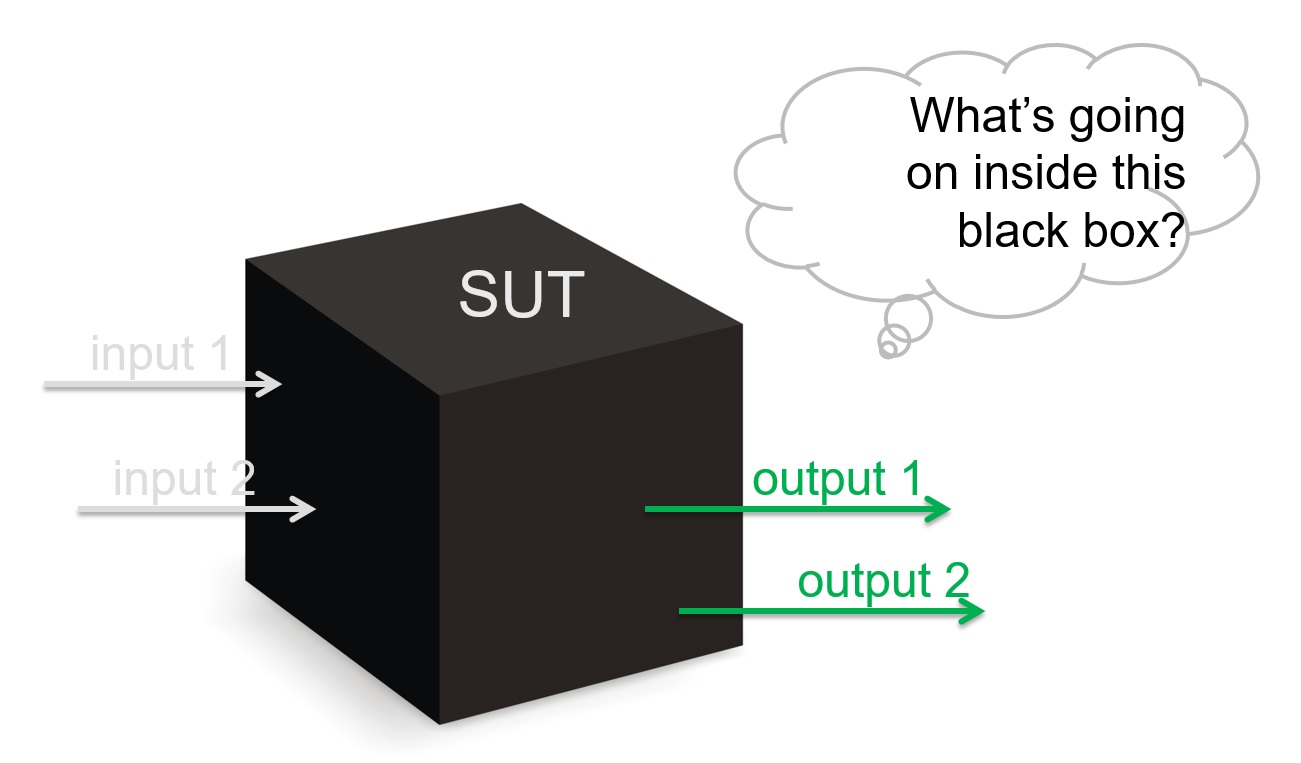
\includegraphics[width=.8\textwidth]{blackbox.jpg}
\end{center}

\pause
\red{Here we assume SUT behaves deterministically and can be reset.}
}

\frame{
	\frametitle{Machine Learning in General}
	
	\begin{center}
		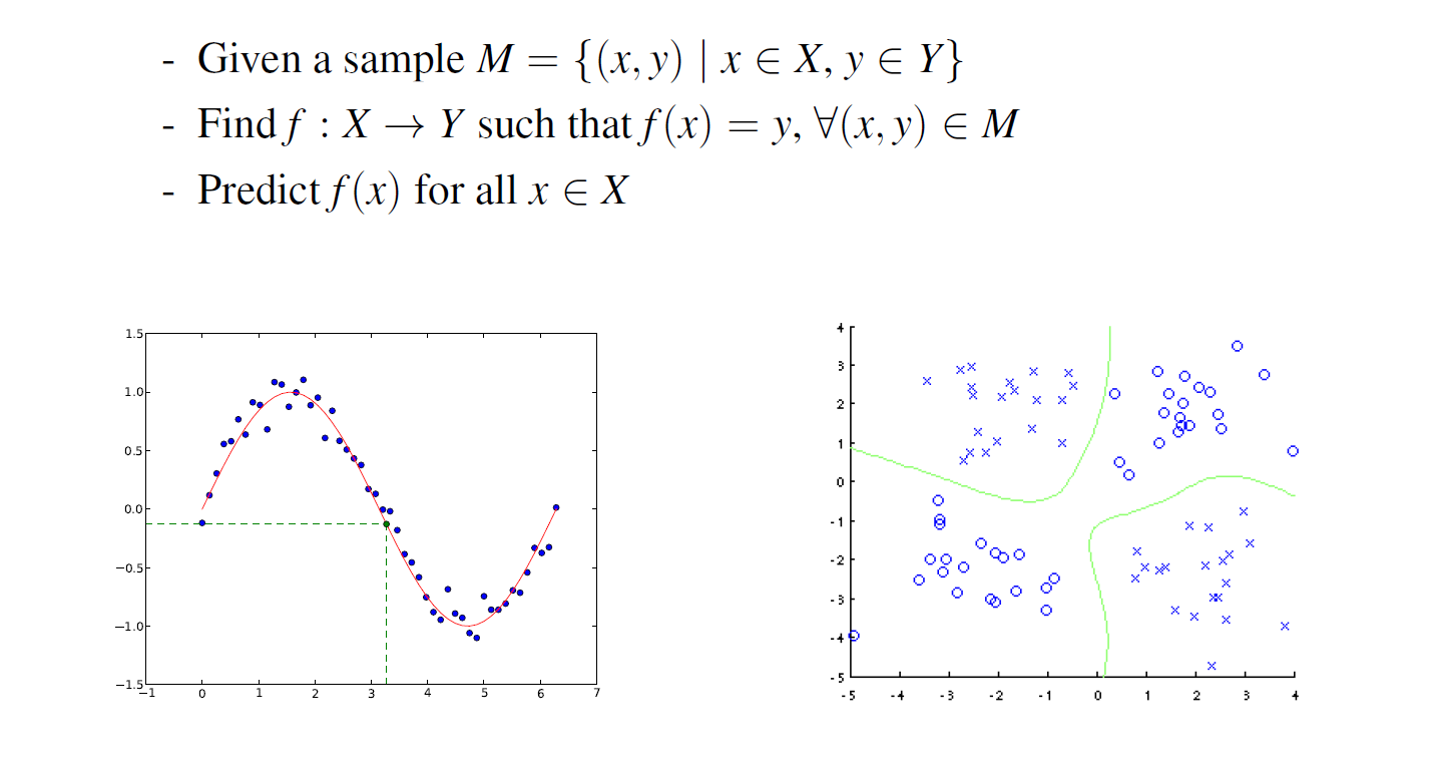
\includegraphics[width=\textwidth]{machinelearningingeneral.png}
	\end{center}
}

\frame{
	\frametitle{Learning Regular Languages}
	
	\begin{center}
		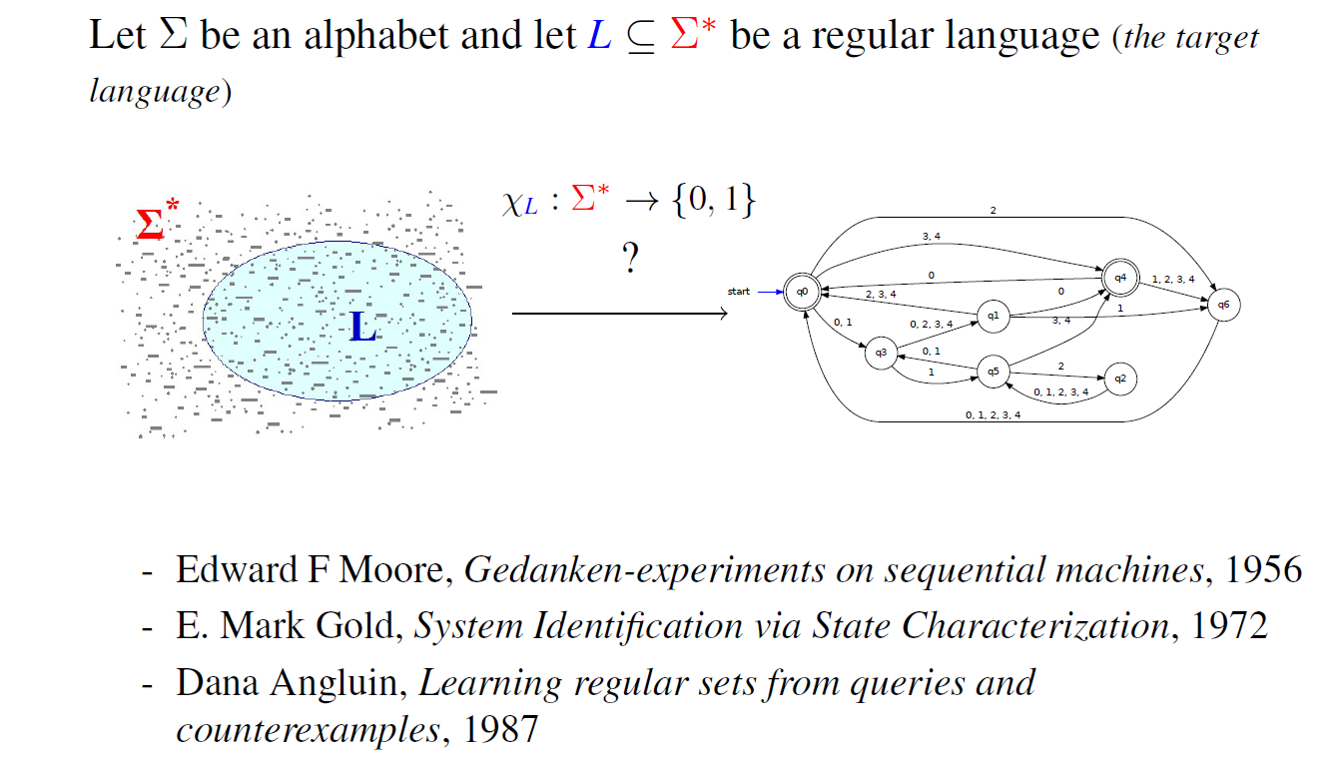
\includegraphics[width=\textwidth]{learningregularlanguages.png}
	\end{center}
}

\frame{
\frametitle{Regular Languages and Congruences}

\begin{definition}
The equivalence relation \red{$\sim_L$}\  on $\Sigma^{\ast}$ induced by a language $L \subseteq \Sigma^{\ast}$:
\begin{eqnarray*}
	u \sim_L v & iff  & \forall w \in \Sigma^{\ast} : u \cdot w \in L \Leftrightarrow v \cdot w \in L
\end{eqnarray*}
\end{definition}

This relation is a right-congruence with respect to concatenation:
\[
\forall u, v, w \in \Sigma^{\ast} : u \sim_L v \Rightarrow u \cdot w \sim_L v \cdot w
\]

\begin{theorem}[Myhill-Nerode, 1958]
	Language $L$ is regular iff $\sim_L$ has finitely equivalence classes.
\end{theorem}
}
\frame{
\frametitle{Visualisation}
Consider the regular language \green{$a (a \mid b)^{\ast} b$}
	
	\begin{center}
		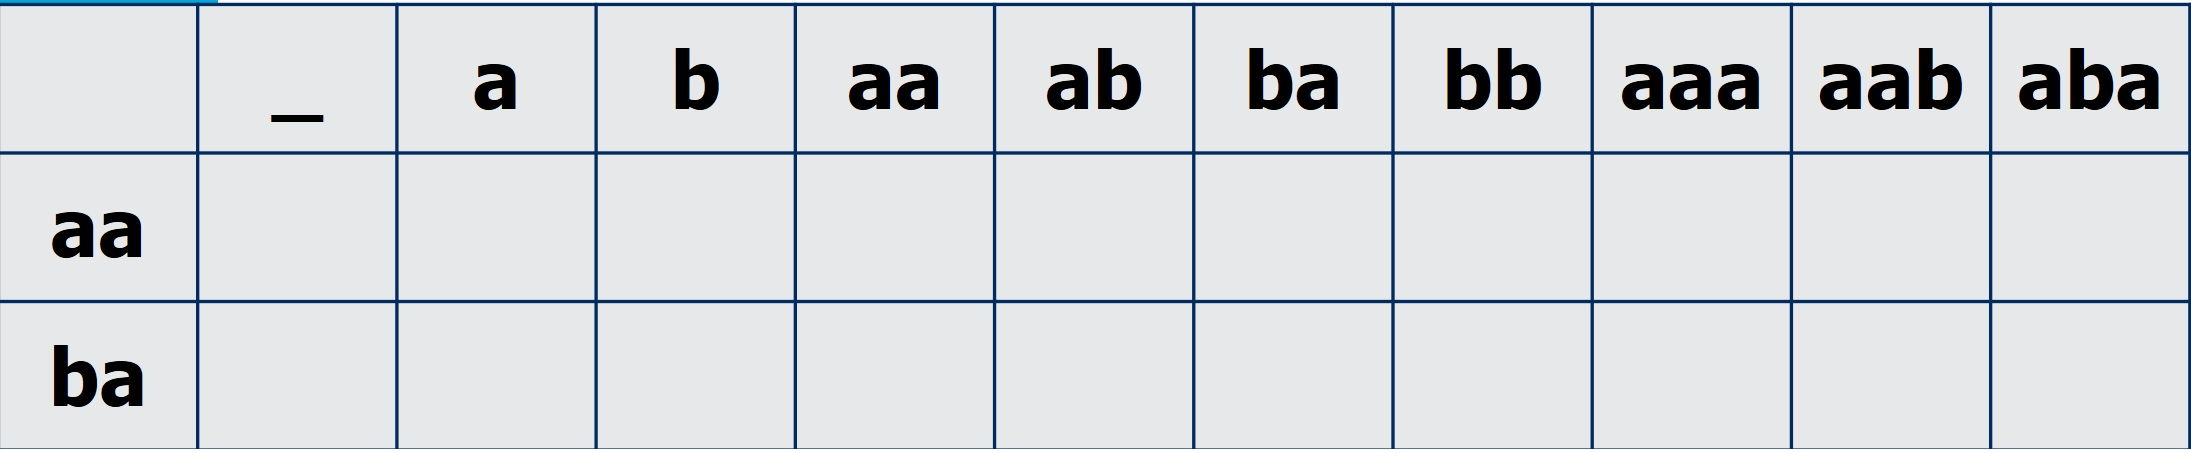
\includegraphics[width=\textwidth]{matrix1.jpg}
	\end{center}
}

\frame{
\frametitle{Visualisation}
Consider the regular language \green{$a (a \mid b)^{\ast} b$}
	
	\begin{center}
		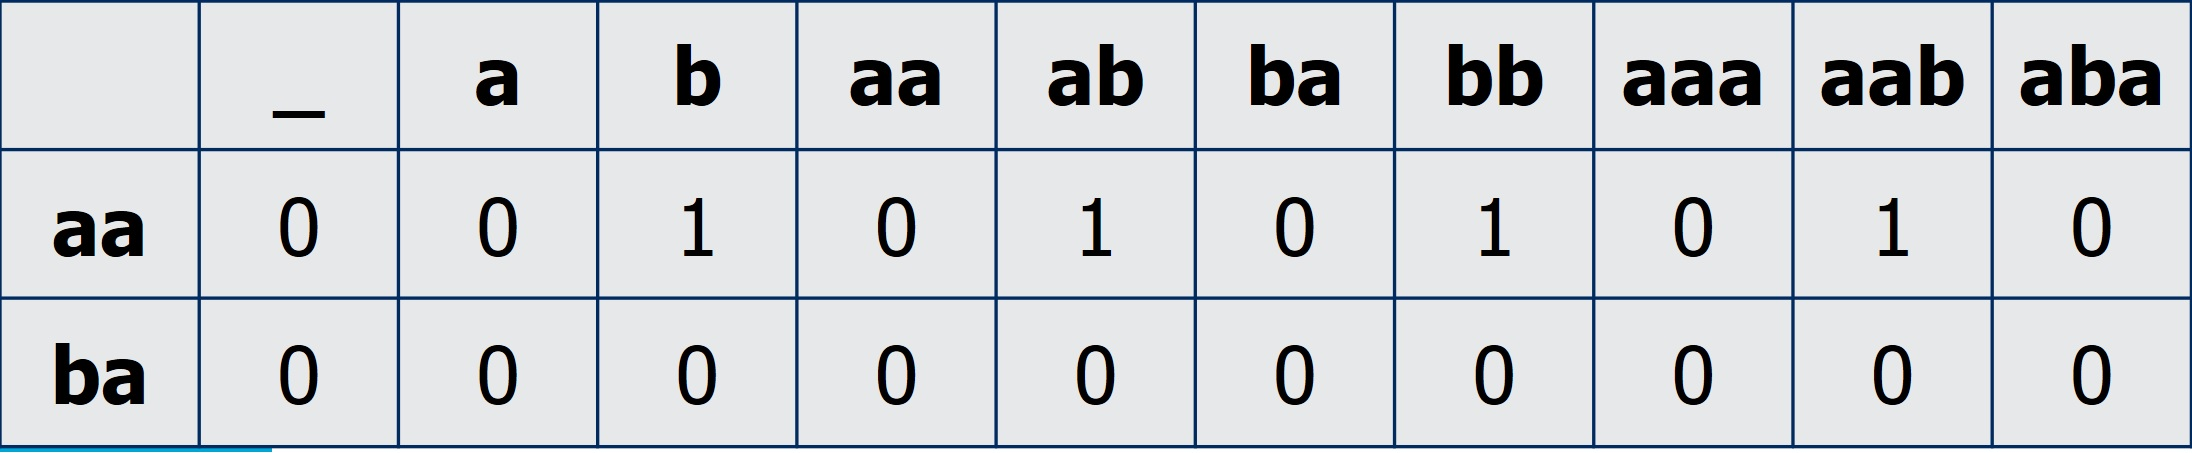
\includegraphics[width=\textwidth]{matrix2.jpg}
	\end{center}
}

\frame{
\frametitle{Hankel Matrix}
	
	\begin{center}
		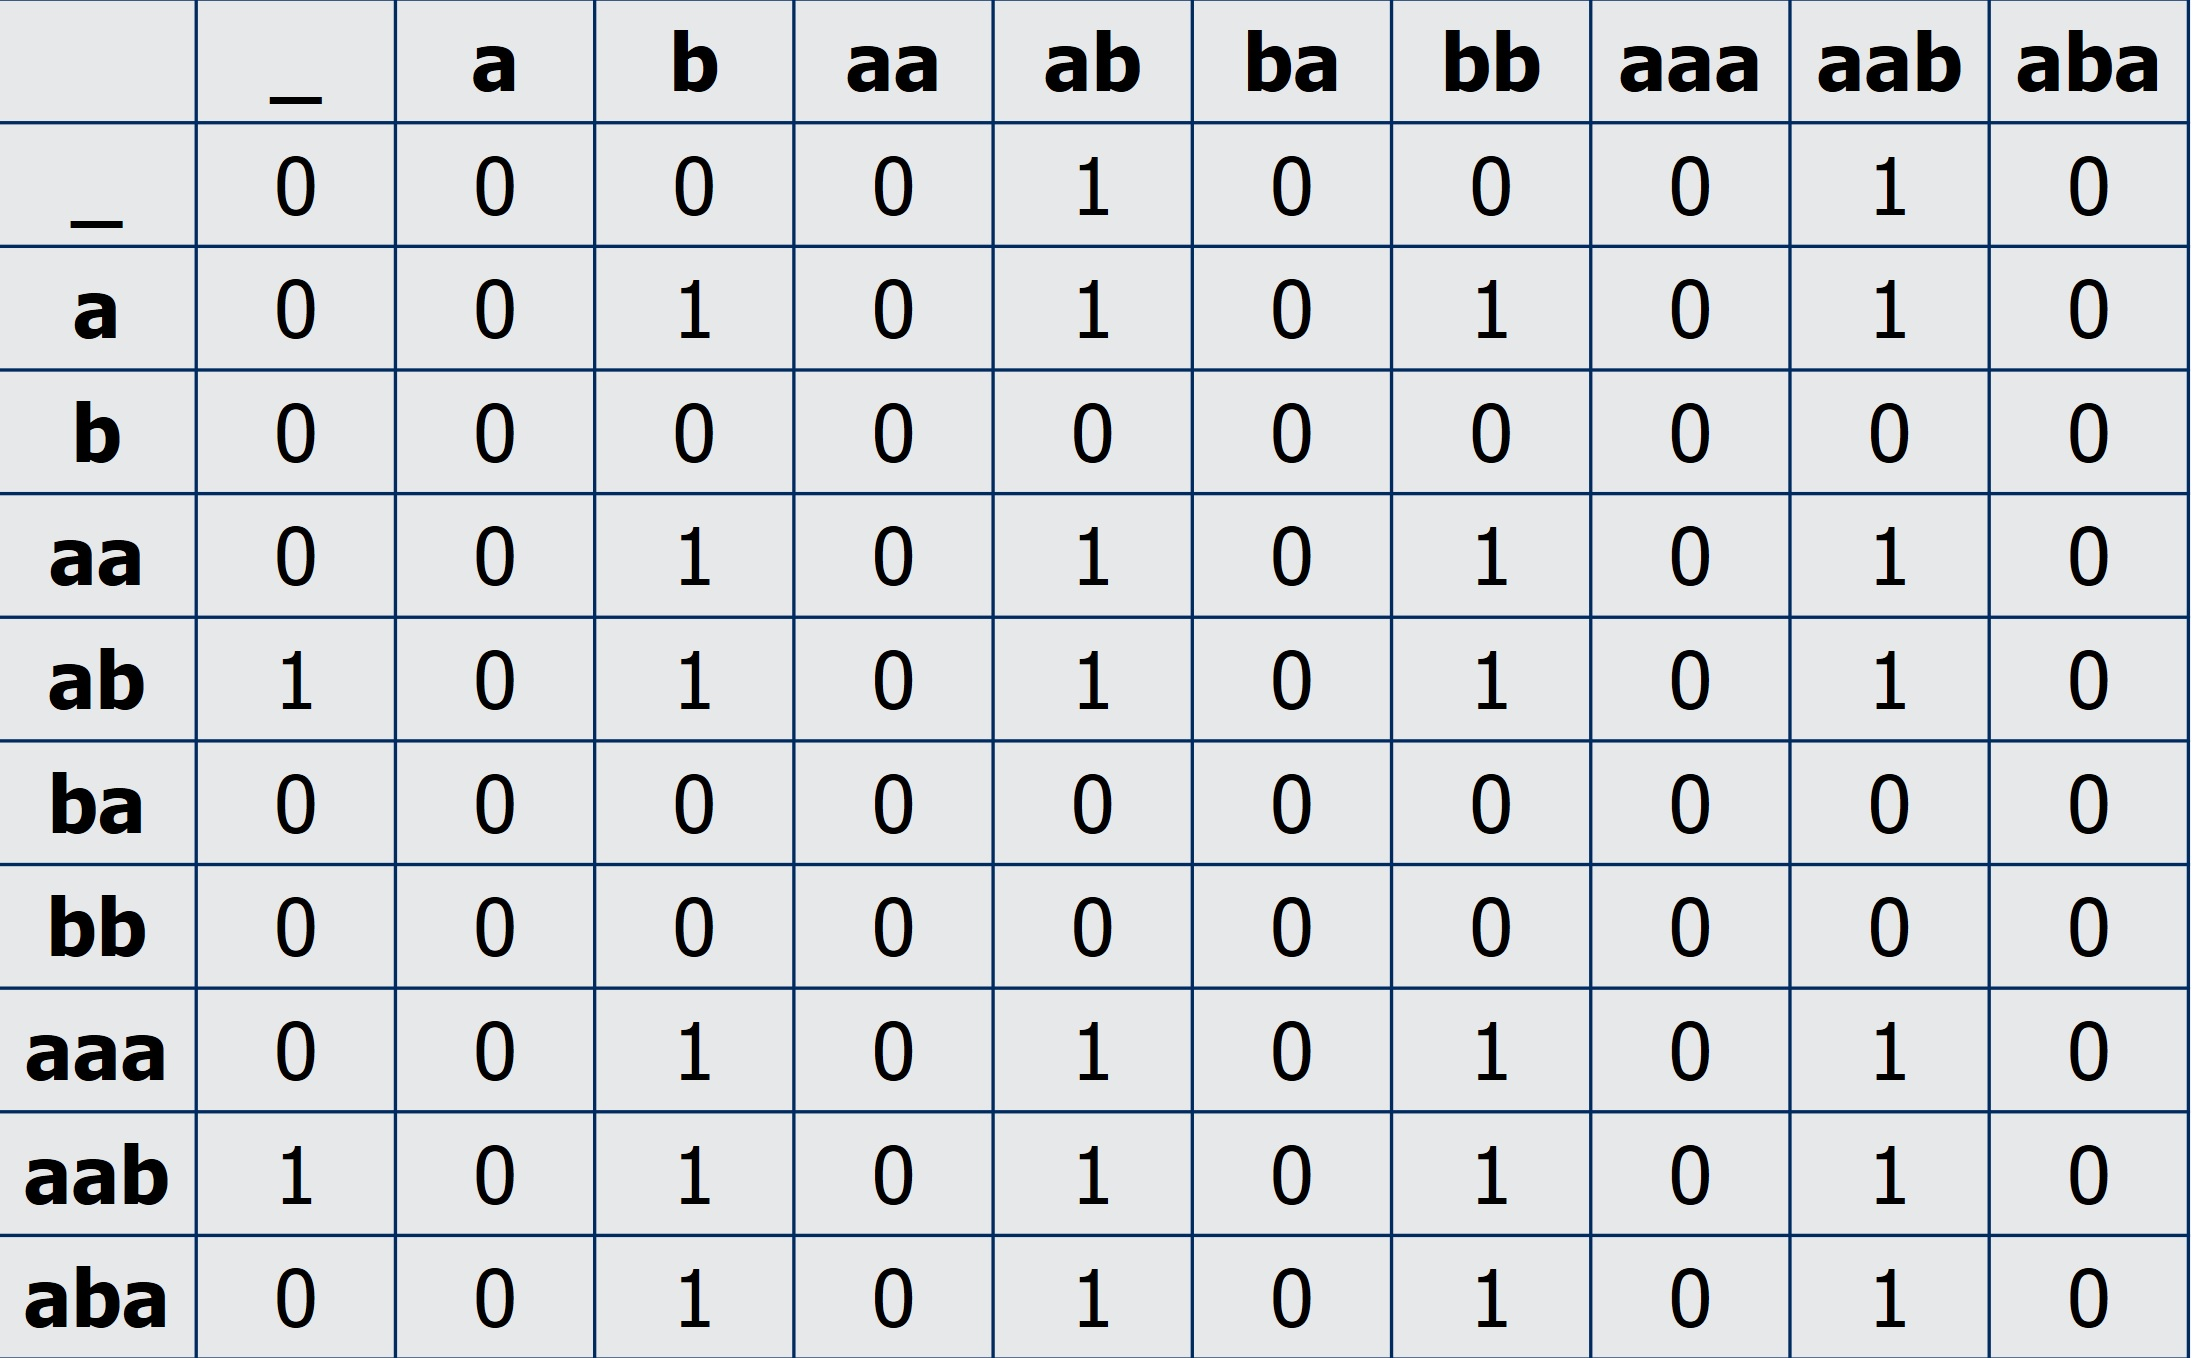
\includegraphics[width=\textwidth]{matrix3.jpg}
	\end{center}
}

\frame{
\frametitle{Hankel Matrix}
	
	\begin{center}
		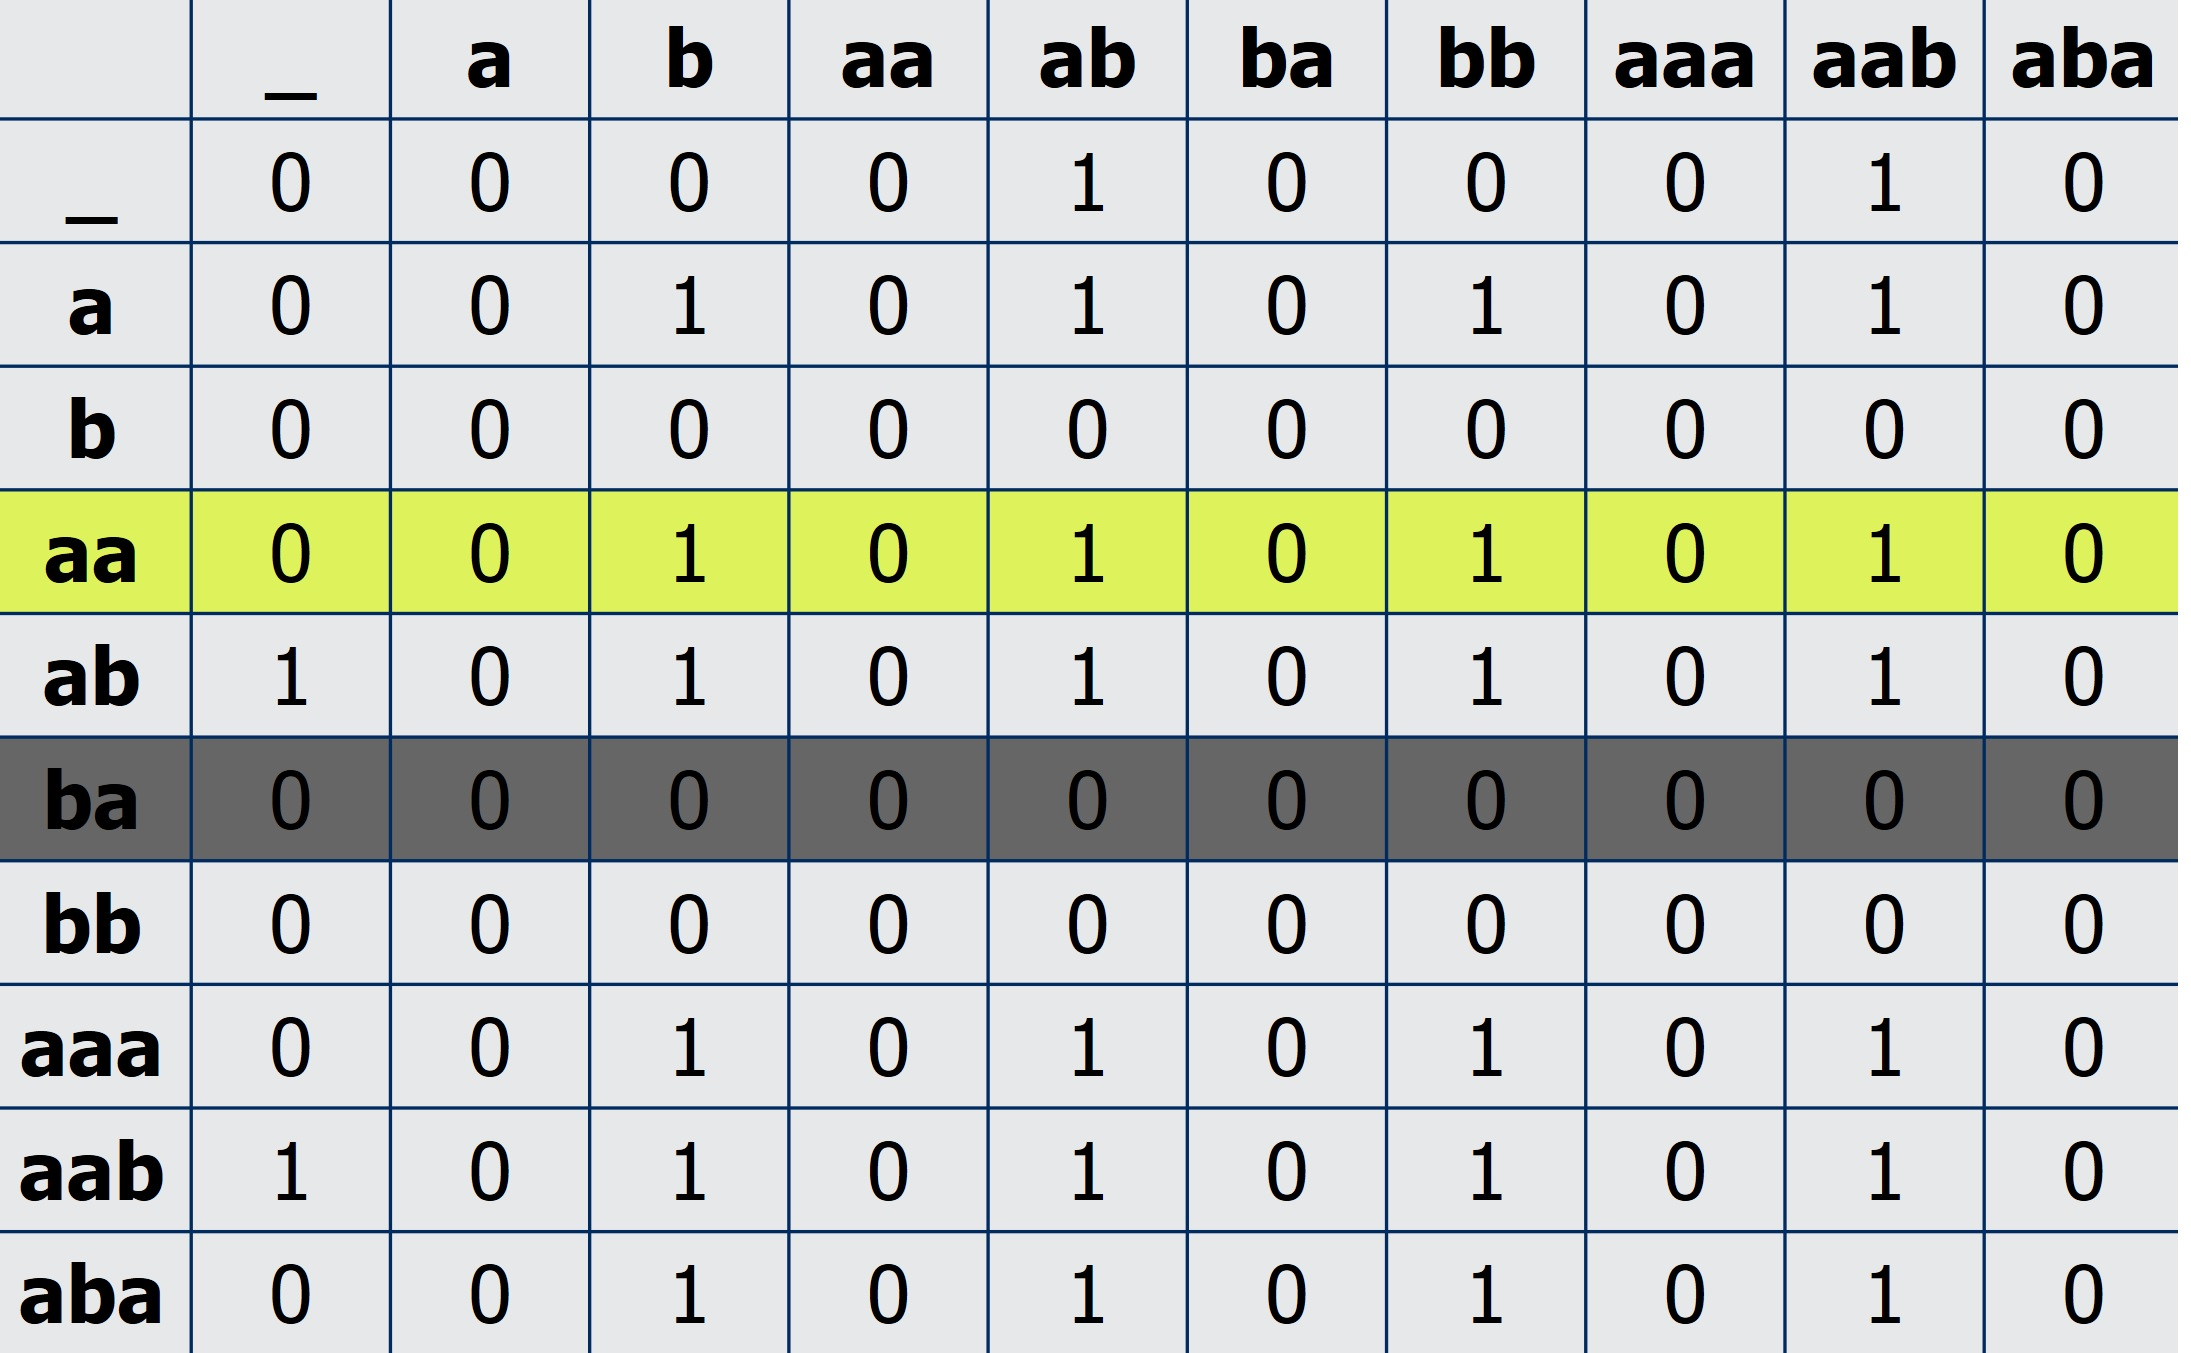
\includegraphics[width=\textwidth]{matrix4.jpg}
	\end{center}
}

\frame{
\frametitle{Hankel Matrix}
	
	\begin{center}
		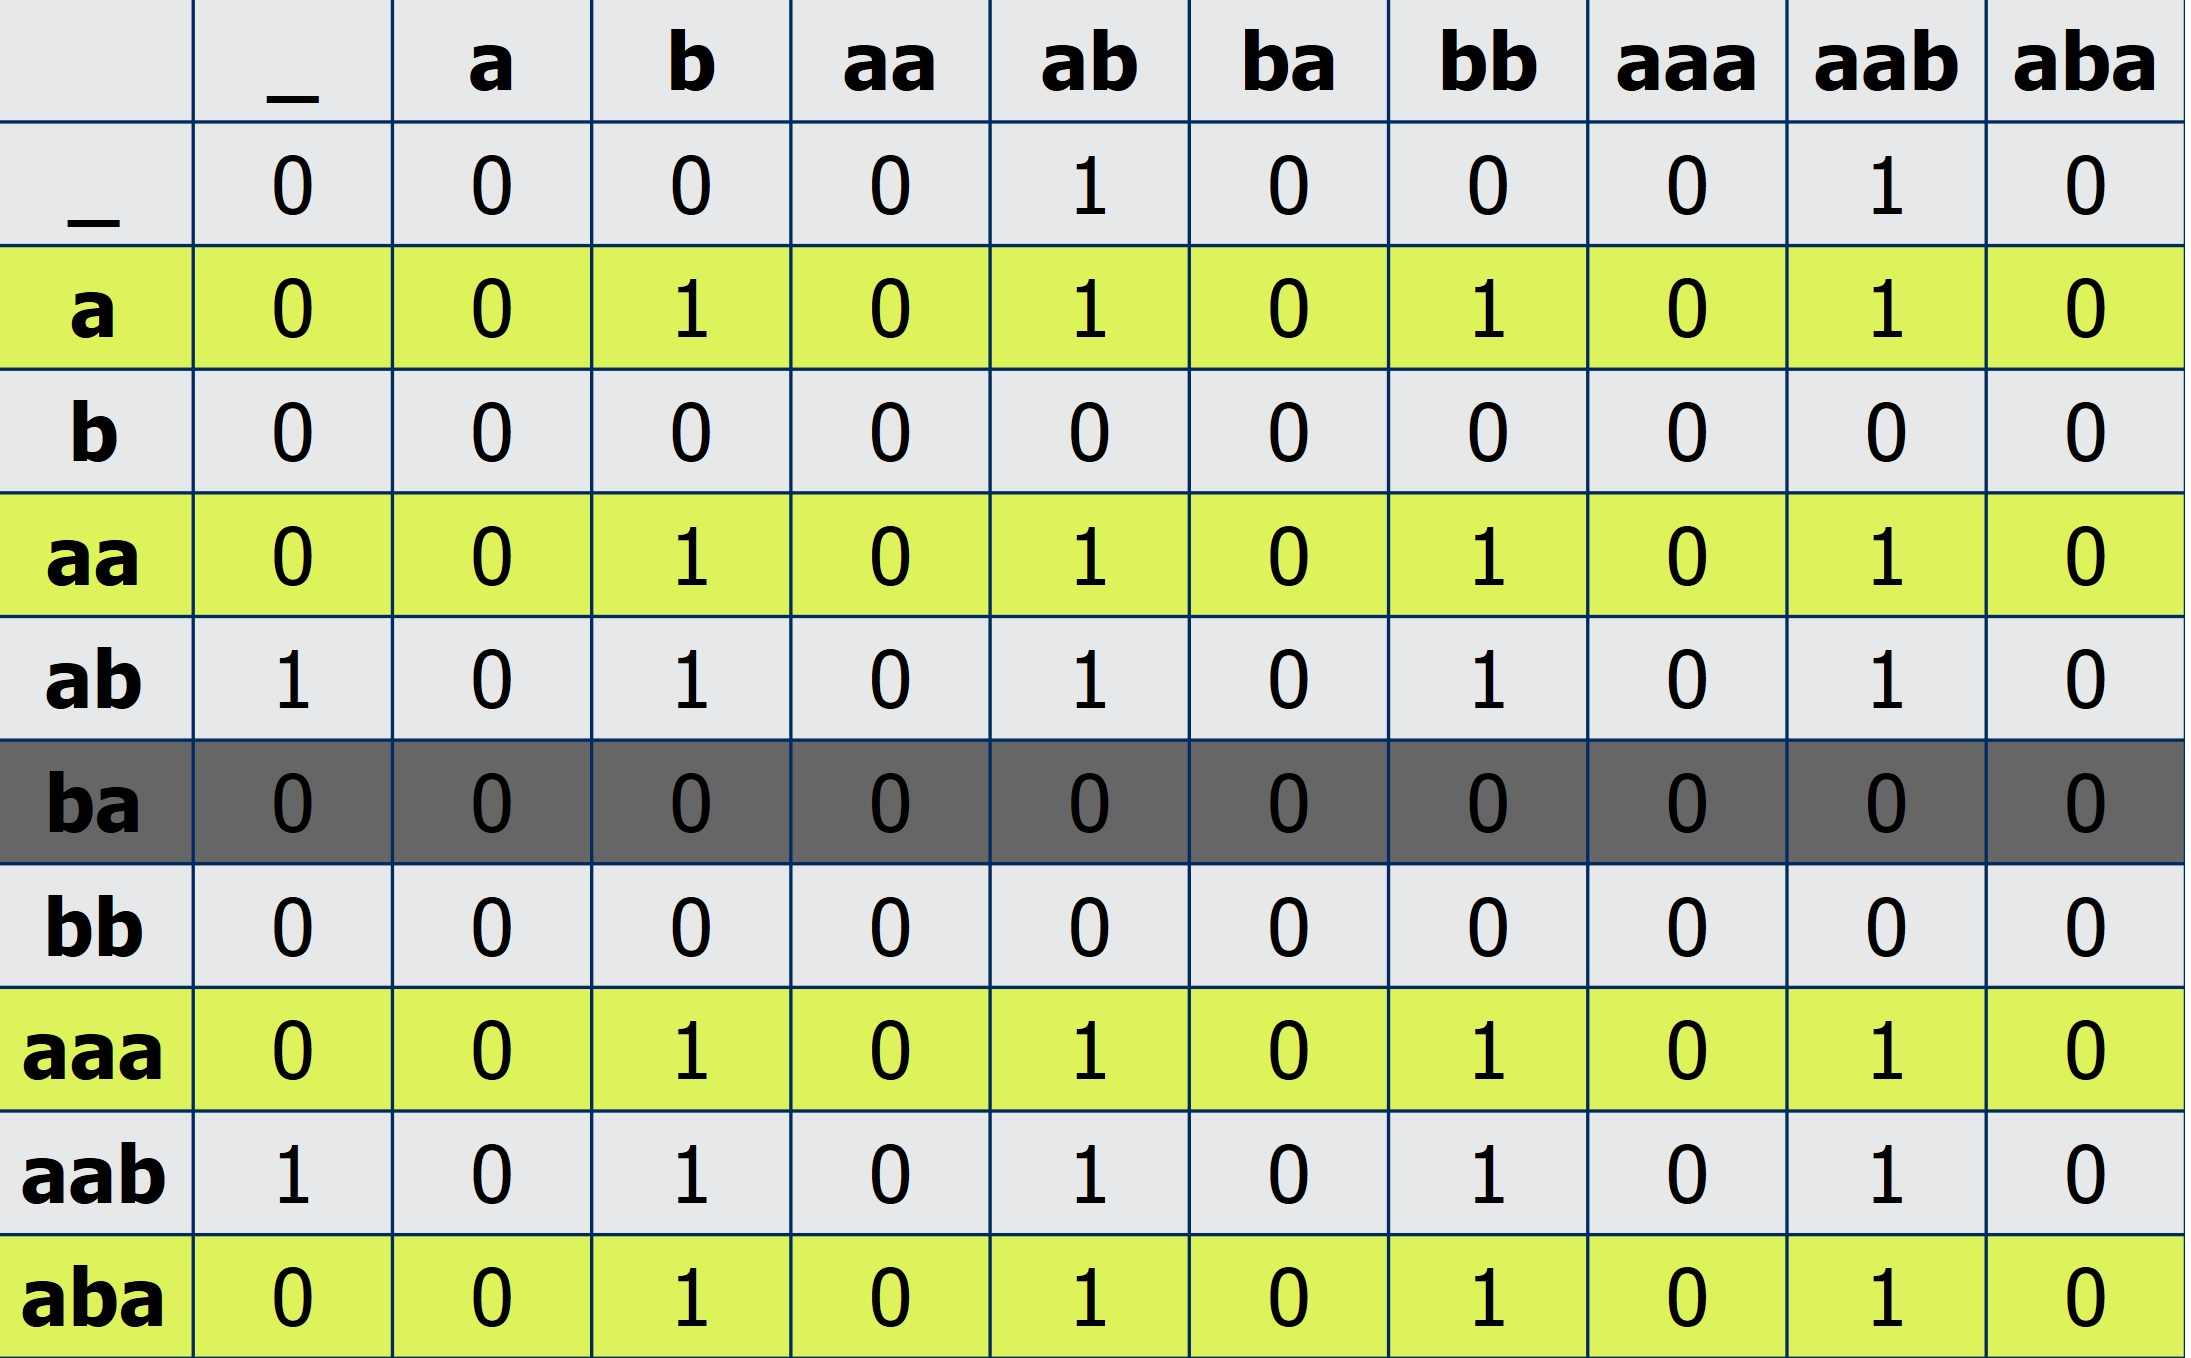
\includegraphics[width=\textwidth]{matrix5.jpg}
	\end{center}
}

\frame{
\frametitle{Hankel Matrix}
	
	\begin{center}
		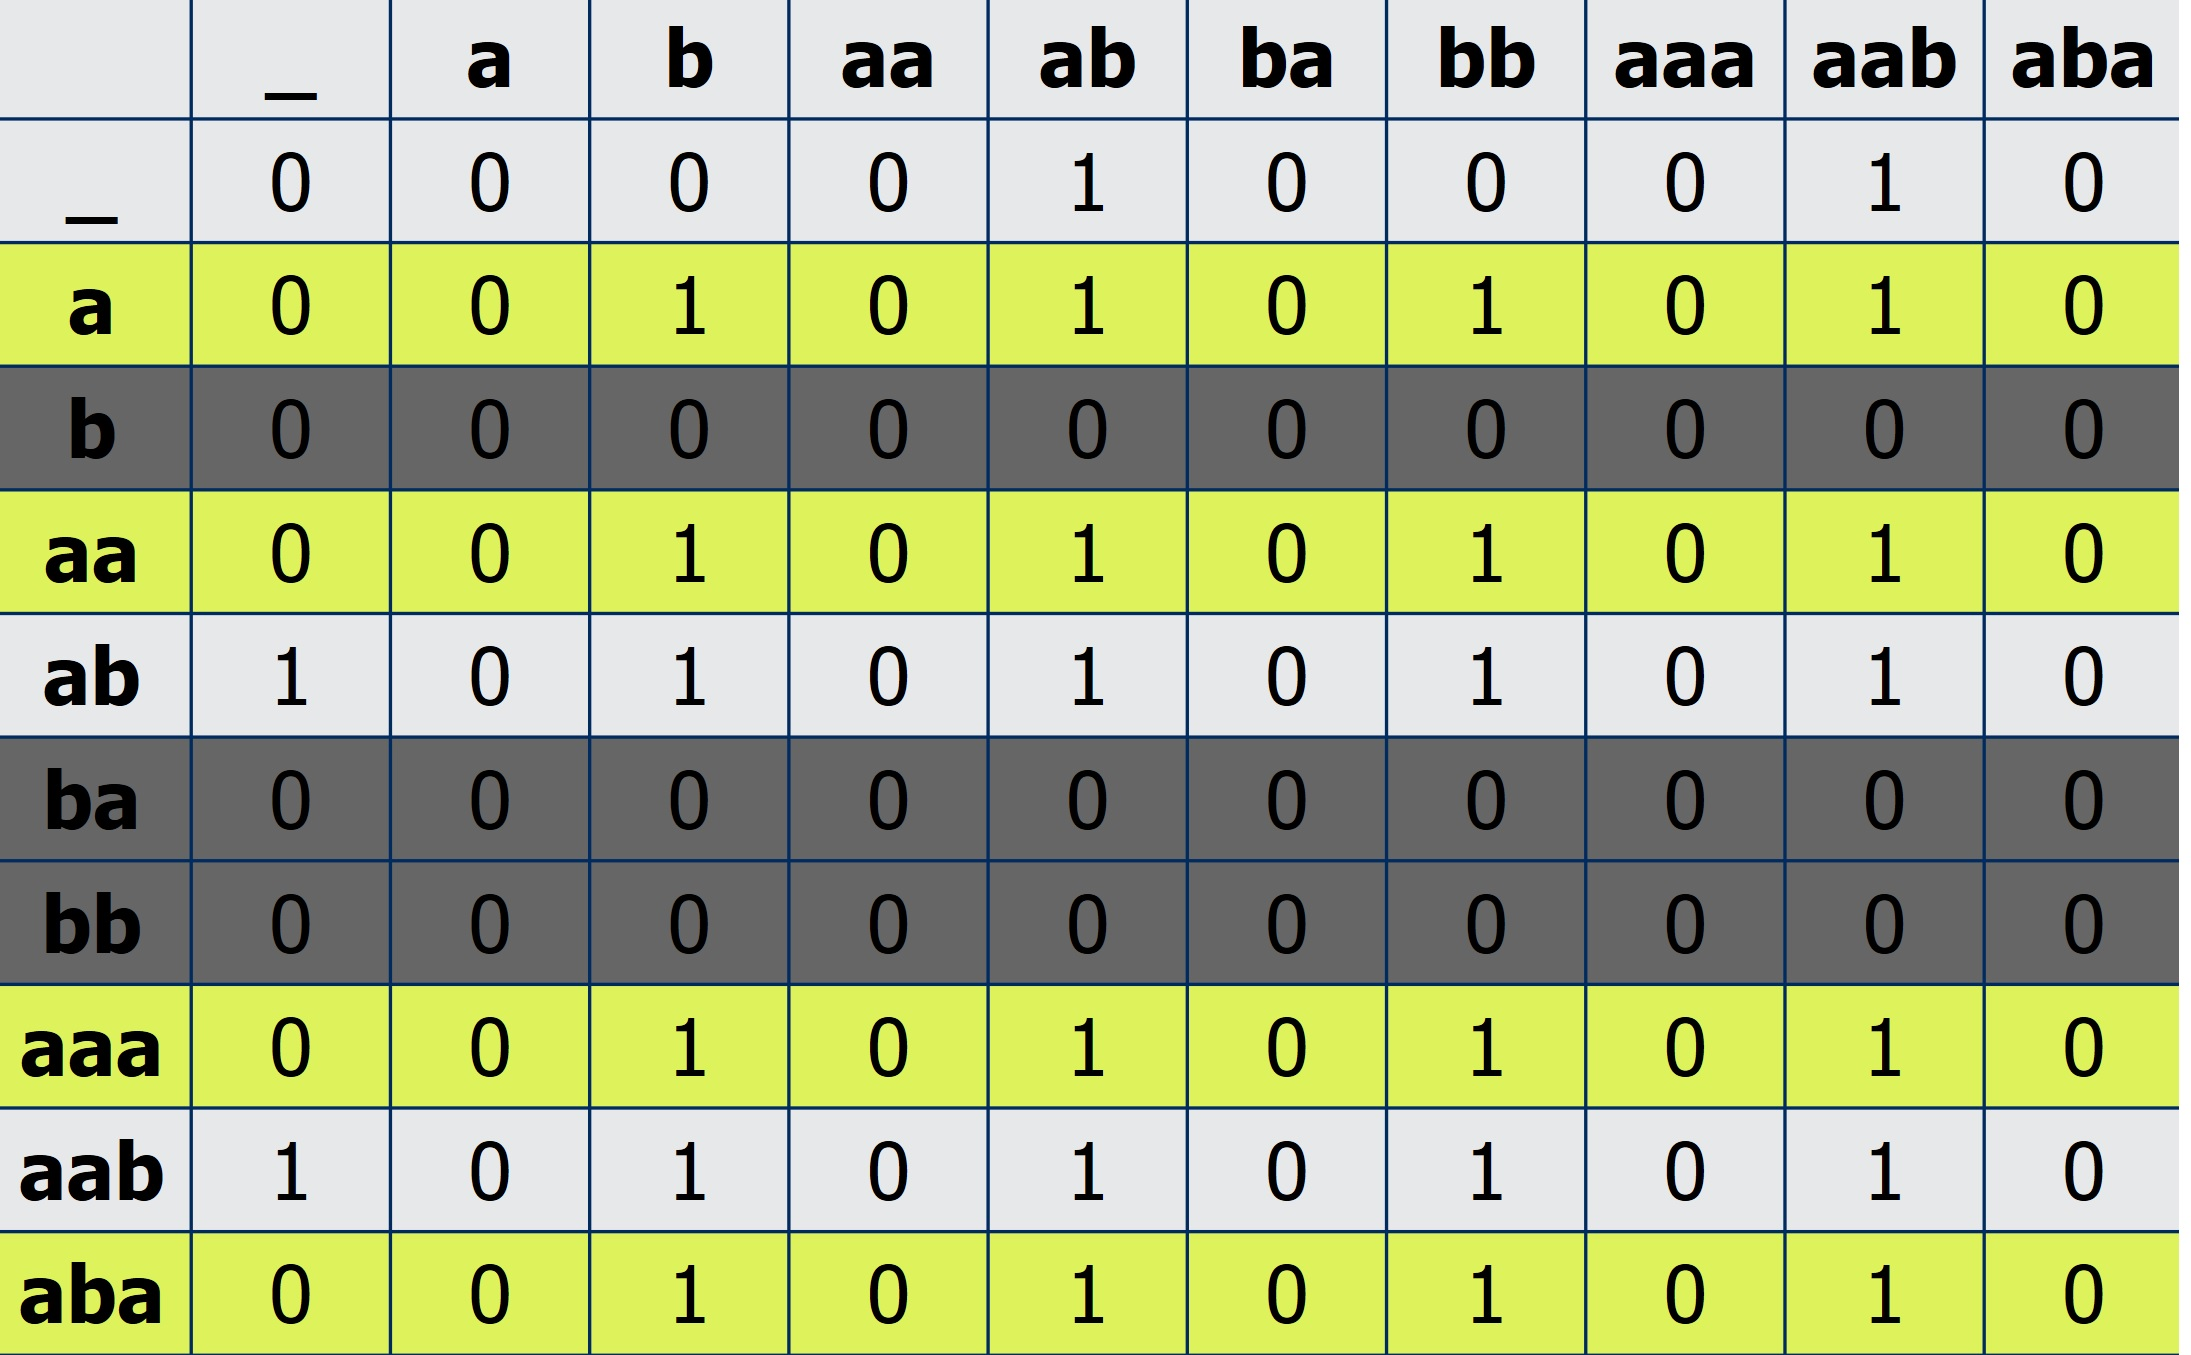
\includegraphics[width=\textwidth]{matrix6.jpg}
	\end{center}
}

\frame{
\frametitle{Hankel Matrix}
	
	\begin{center}
		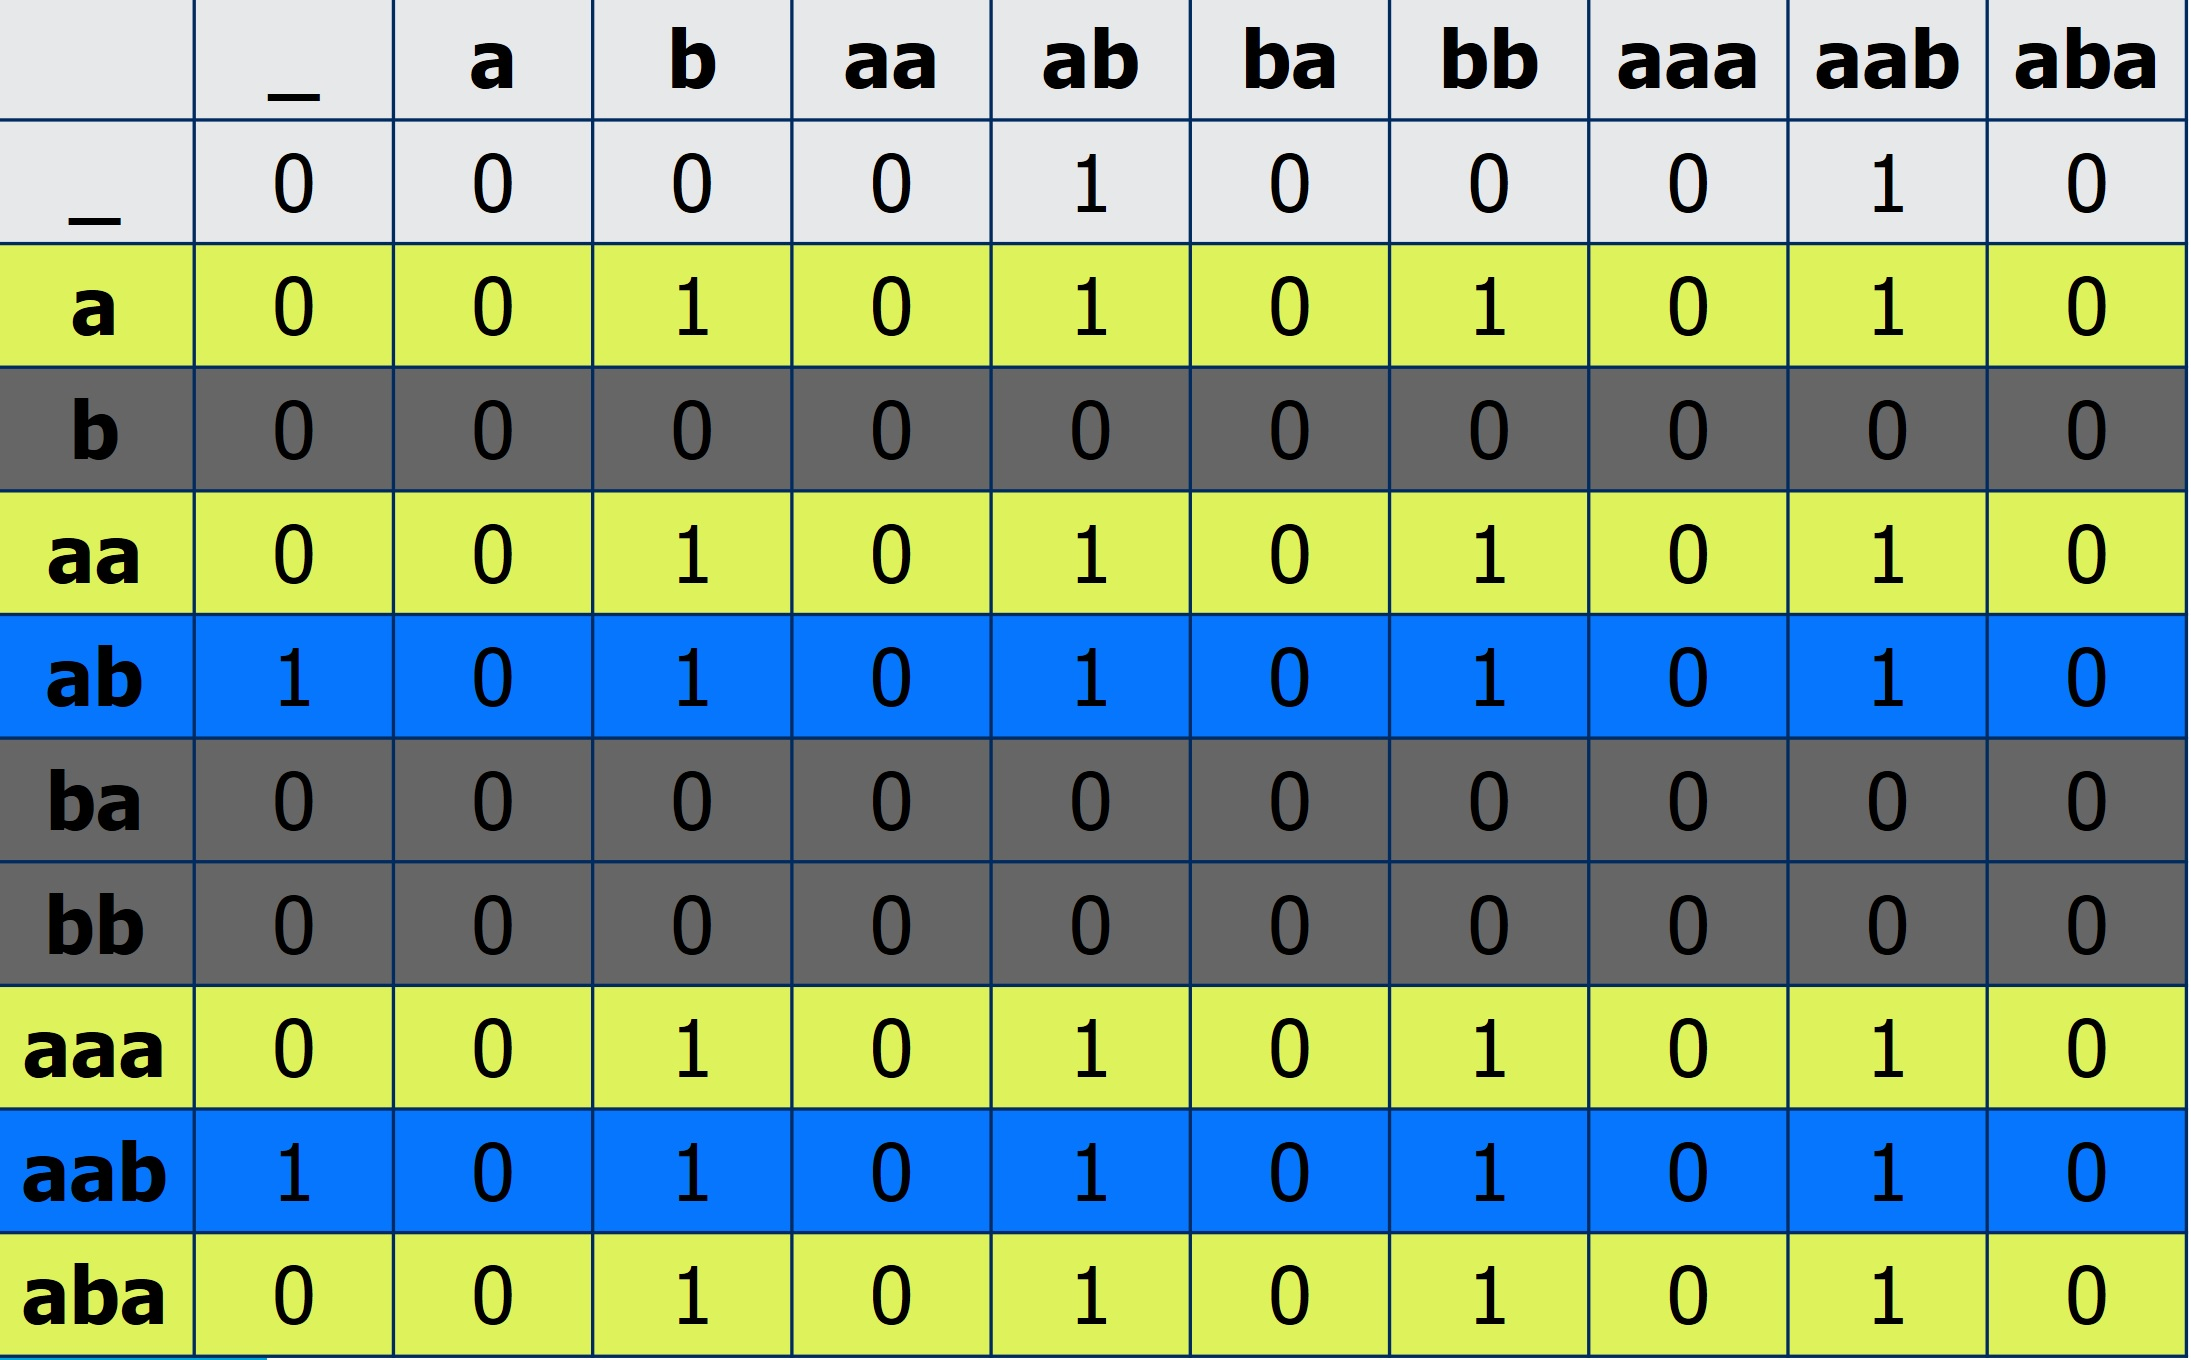
\includegraphics[width=\textwidth]{matrix7.jpg}
	\end{center}
}


\frame{
\frametitle{Hankel Matrix}	
	\begin{center}
		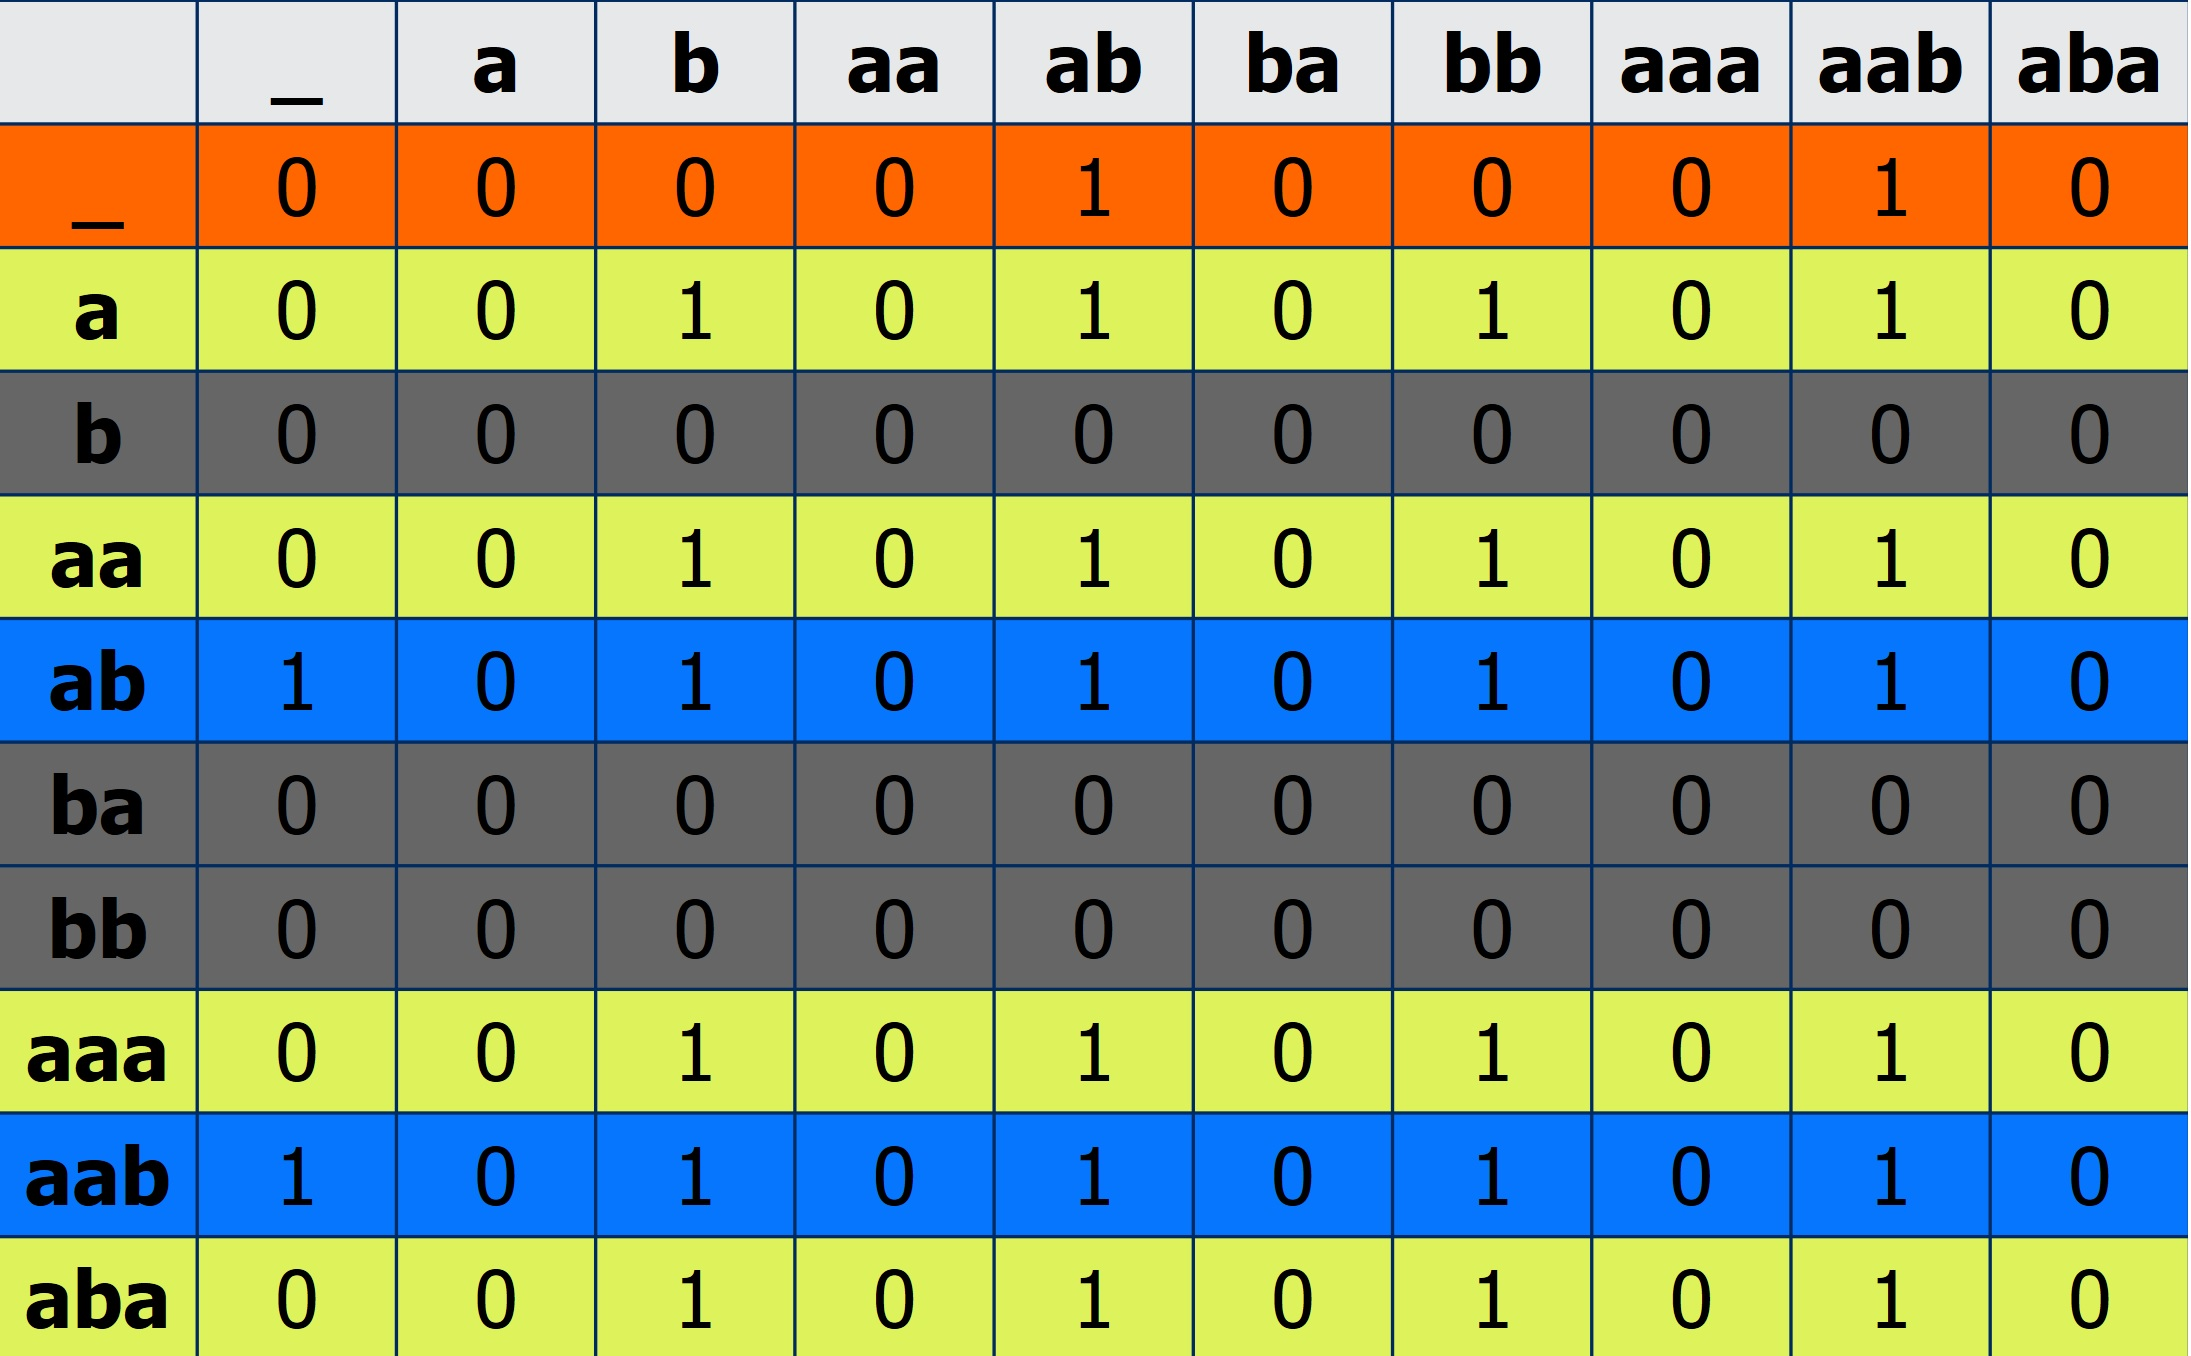
\includegraphics[width=\textwidth]{matrix8.jpg}
	\end{center}
}



\frame{
	\frametitle{Hankel Matrix}
\begin{itemize}
	\item 
	
	$u \sim_L v$ iff rows of $u$ and $v$ in Hankel matrix for $L$ have the same color
\pause	
\item
	Language $L$ is regular iff its Hankel matrix contains a \red{finite number of distinct rows}, i.e., colors
\pause	
\item
	The number of states in the smallest DFA for $L$ equals \red{the number of colors in the Hankel matrix}
\end{itemize}	
}


\frame{
	\frametitle{What is the FSM for this Hankel Matrix?}
	
	\begin{center}
		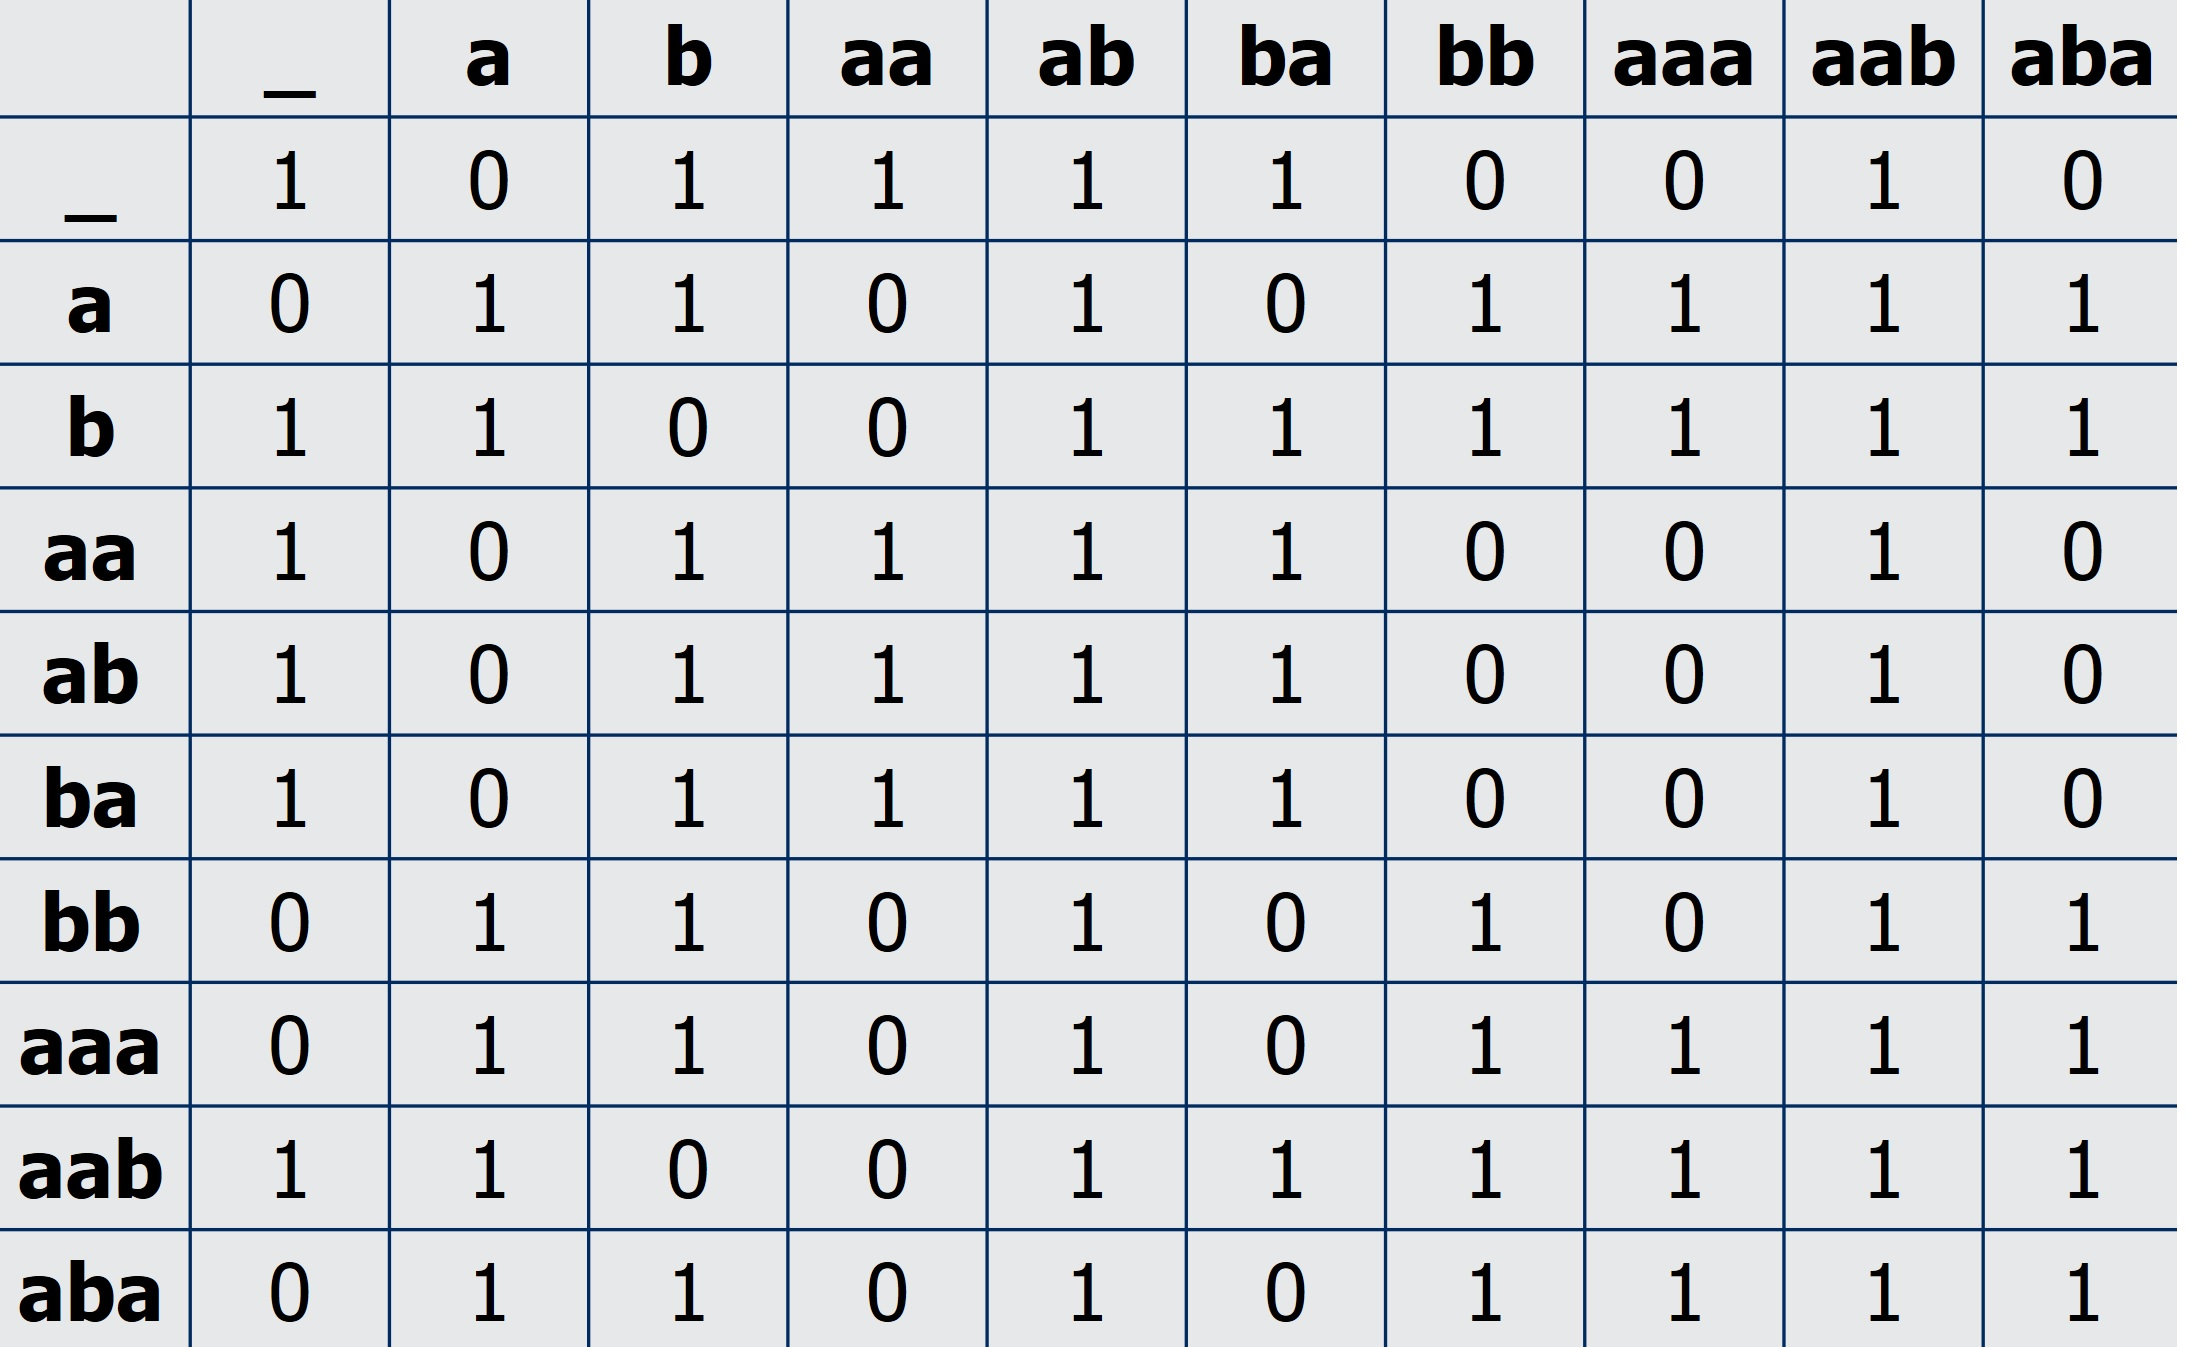
\includegraphics[width=\textwidth]{matrix9.jpg}
	\end{center}
}



\frame{
	\frametitle{What is the FSM for this Hankel Matrix?}	
	\begin{center}
		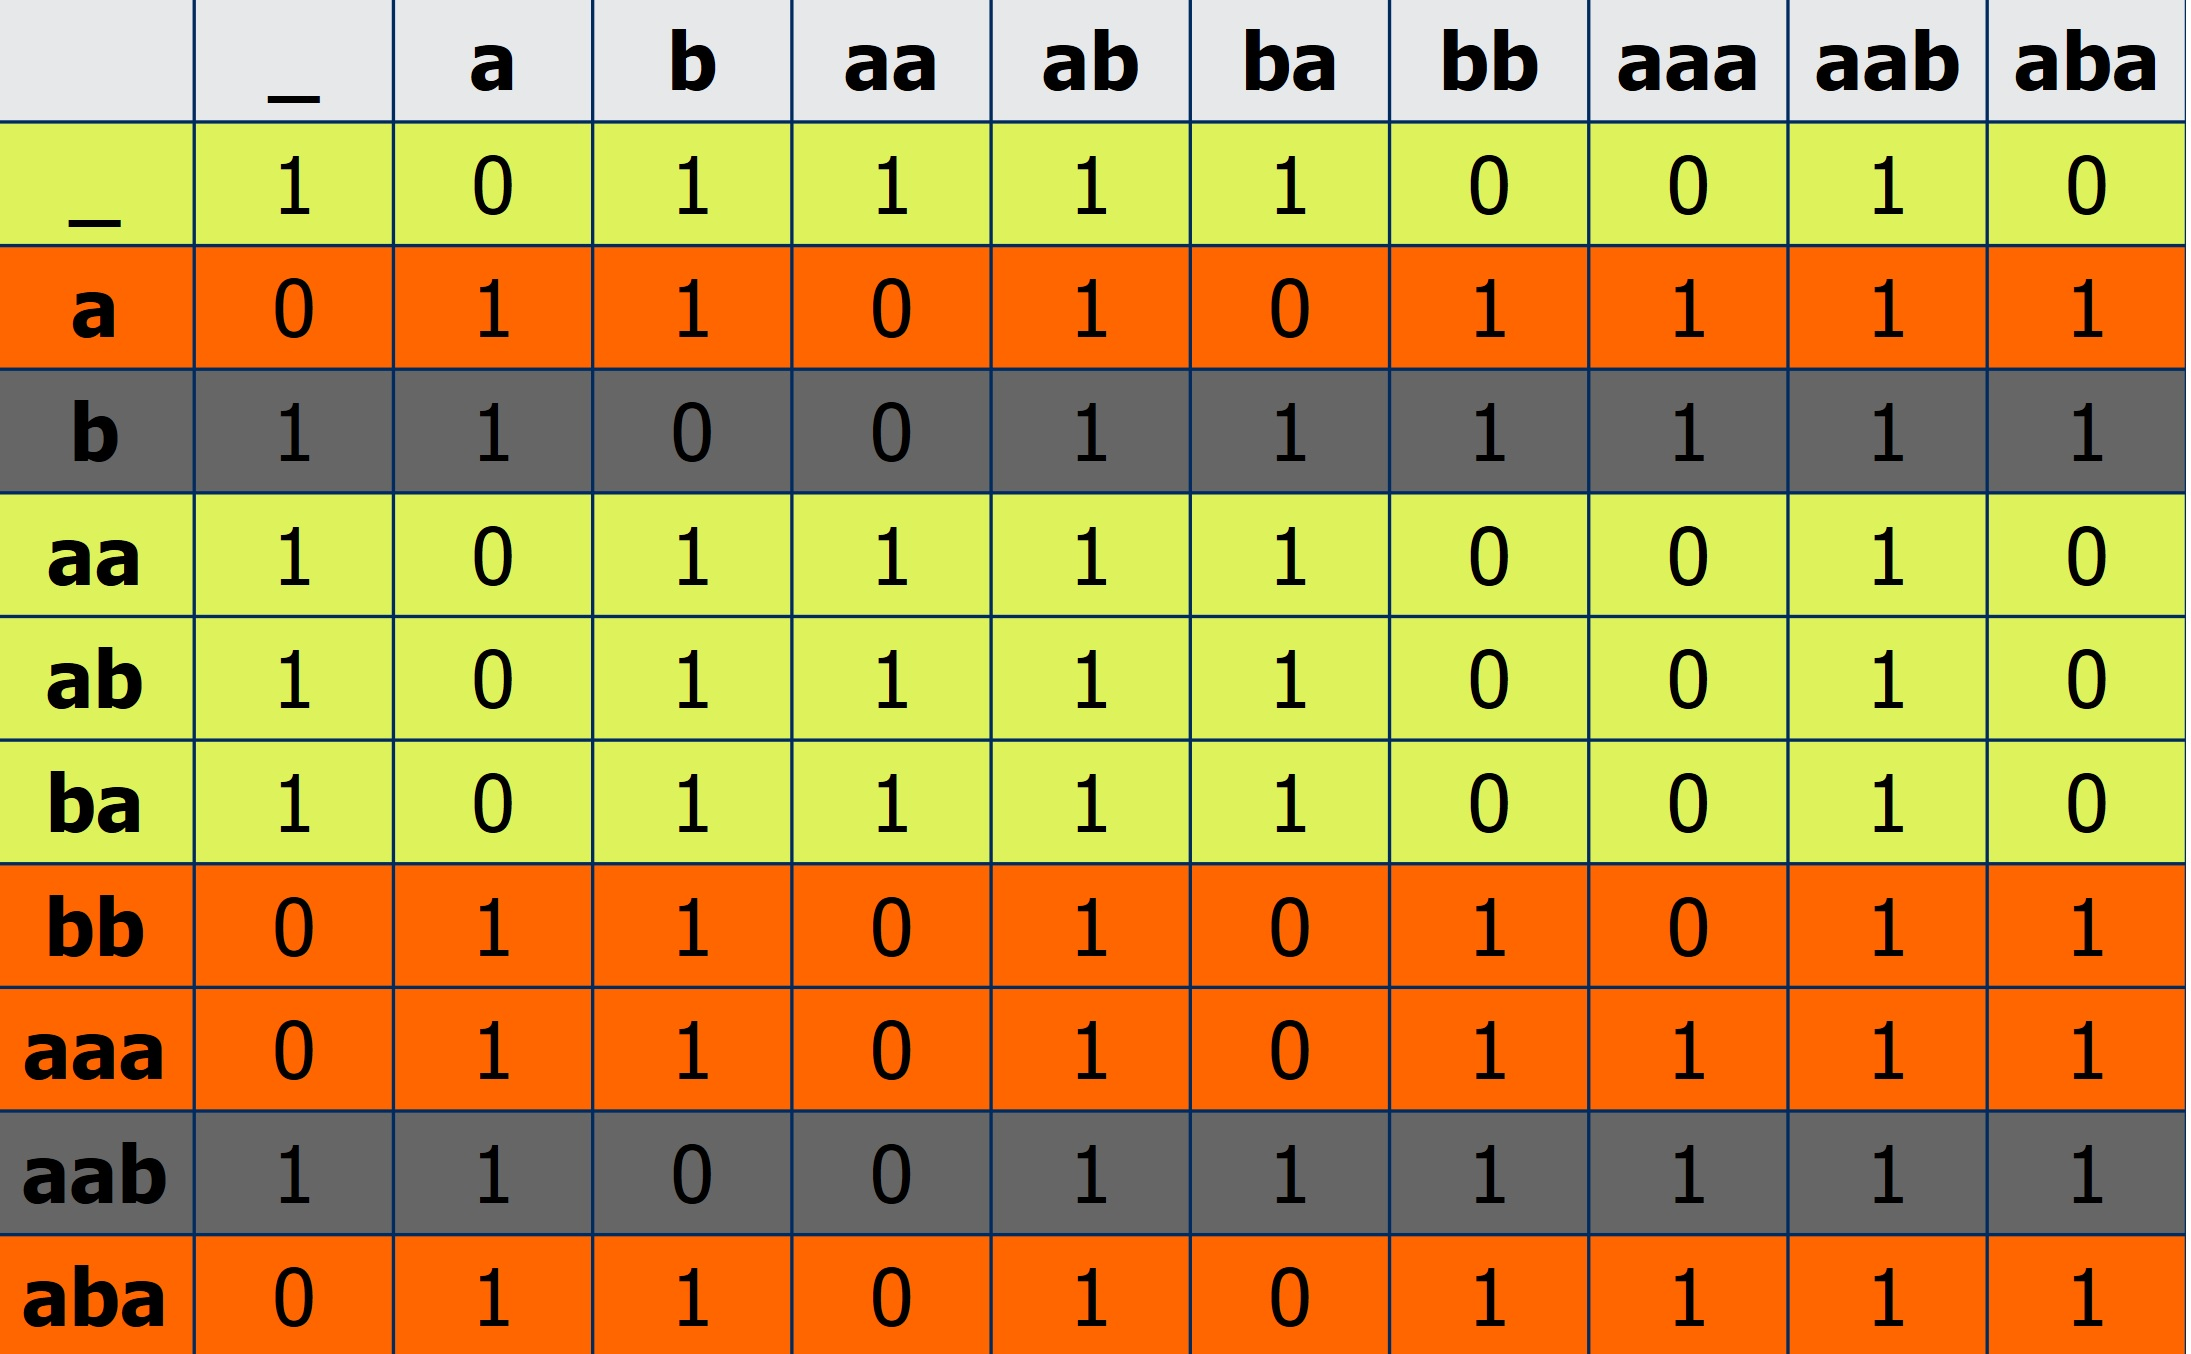
\includegraphics[width=\textwidth]{matrix10.jpg}
	\end{center}
}

\frame{
	\frametitle{Solution}
	\begin{center}
		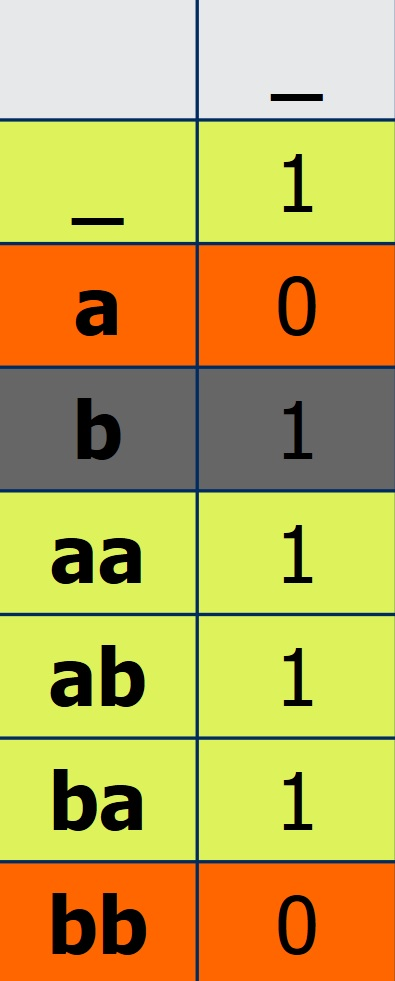
\includegraphics[width=1.5cm]{matrix11.jpg}
		\hspace{1cm}
		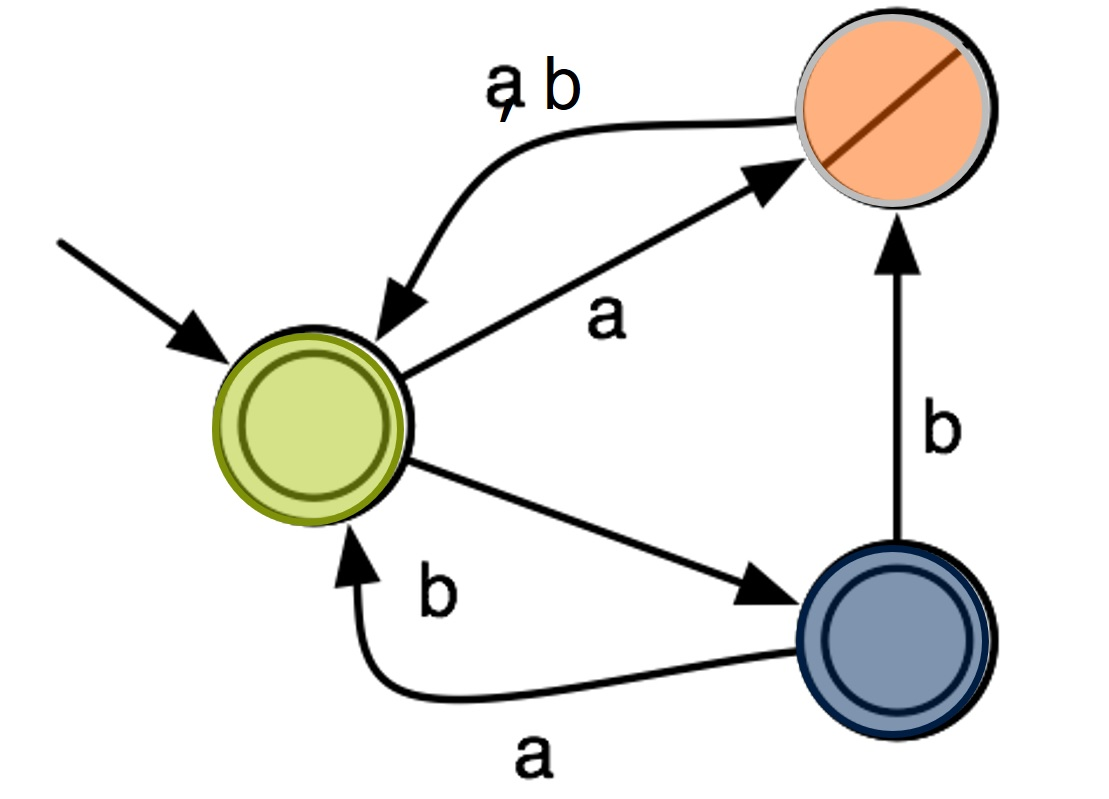
\includegraphics[width=5cm]{DFAsicco.jpg}
	\end{center}

Colors of rows in Hankel matrix give us the states.

Access strings and one-letter extensions allow us to determine transitions.

Column for empty suffix gives us the accepting states. 
}


\frame{
	\frametitle{What if Hankel Matrix is Incomplete?}	
	\begin{center}
		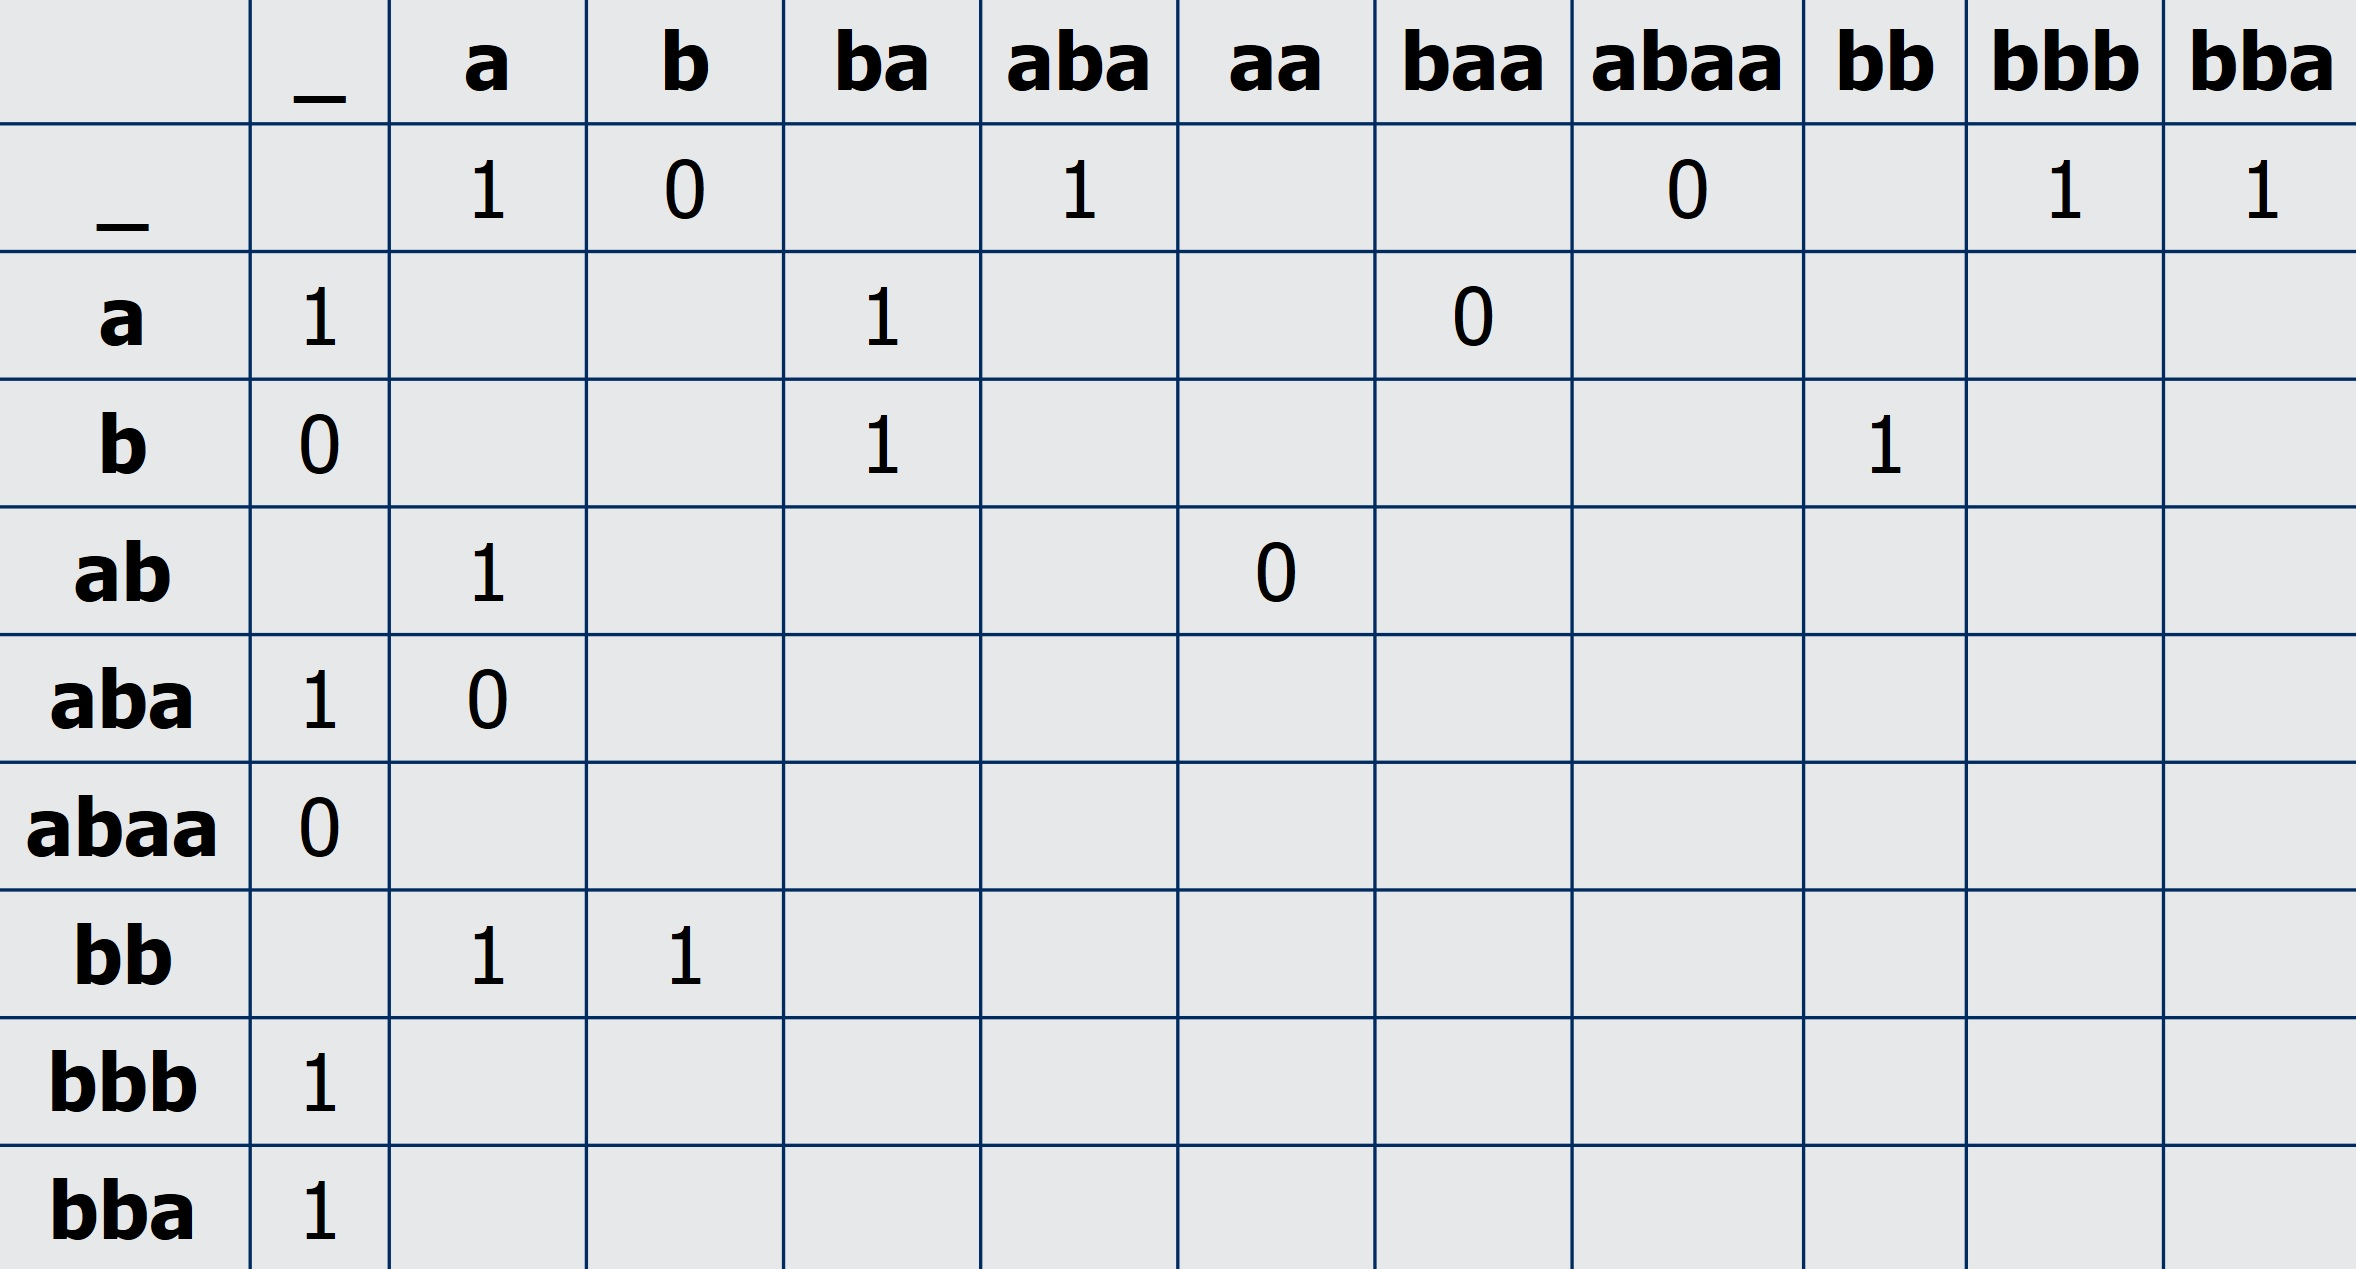
\includegraphics[width=\textwidth]{matrix12.jpg}
	\end{center}
\red{Problem to color such a matrix is NP-hard!}
}

\frame{
\frametitle{Minimally Adequate Teacher (Angluin)}

\begin{center}
	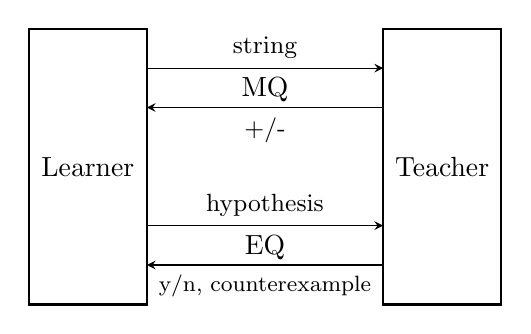
\begin{tikzpicture}[>=stealth]
	\draw [thick] (0,0) rectangle (1.5,3.5) node[midway] {Learner};
	\draw [thick] (4.5,0) rectangle (6,3.5) node[midway] {Teacher};
	\draw [->] (1.5,3) -- (4.5,3) node[midway,below] {MQ};
	\draw (1.5,3) -- (4.5,3) node[midway,above] {\small string};
	\draw [<-] (1.5,2.5) -- (4.5,2.5) node[midway,below] {\small +/-};
	\draw [->] (1.5,1) -- (4.5,1) node[midway,below] {EQ};
	\draw (1.5,1) -- (4.5,1) node[midway,above] {\small hypothesis};
	\draw [<-] (1.5,0.5) -- (4.5,0.5) node[midway,below] {\footnotesize y/n, counterexample};
	\end{tikzpicture}
	\hspace{2 em}
	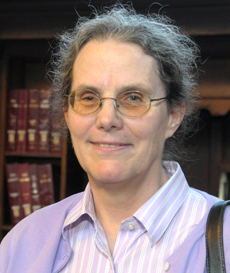
\includegraphics[width=.25\textwidth]{angluin.png}
\end{center}

Learner asks \red{membership queries}\ and \red{equivalence queries}
}

\frame{
\frametitle{Angluin's $L^{\ast}$ Algorithm}

\begin{center}
	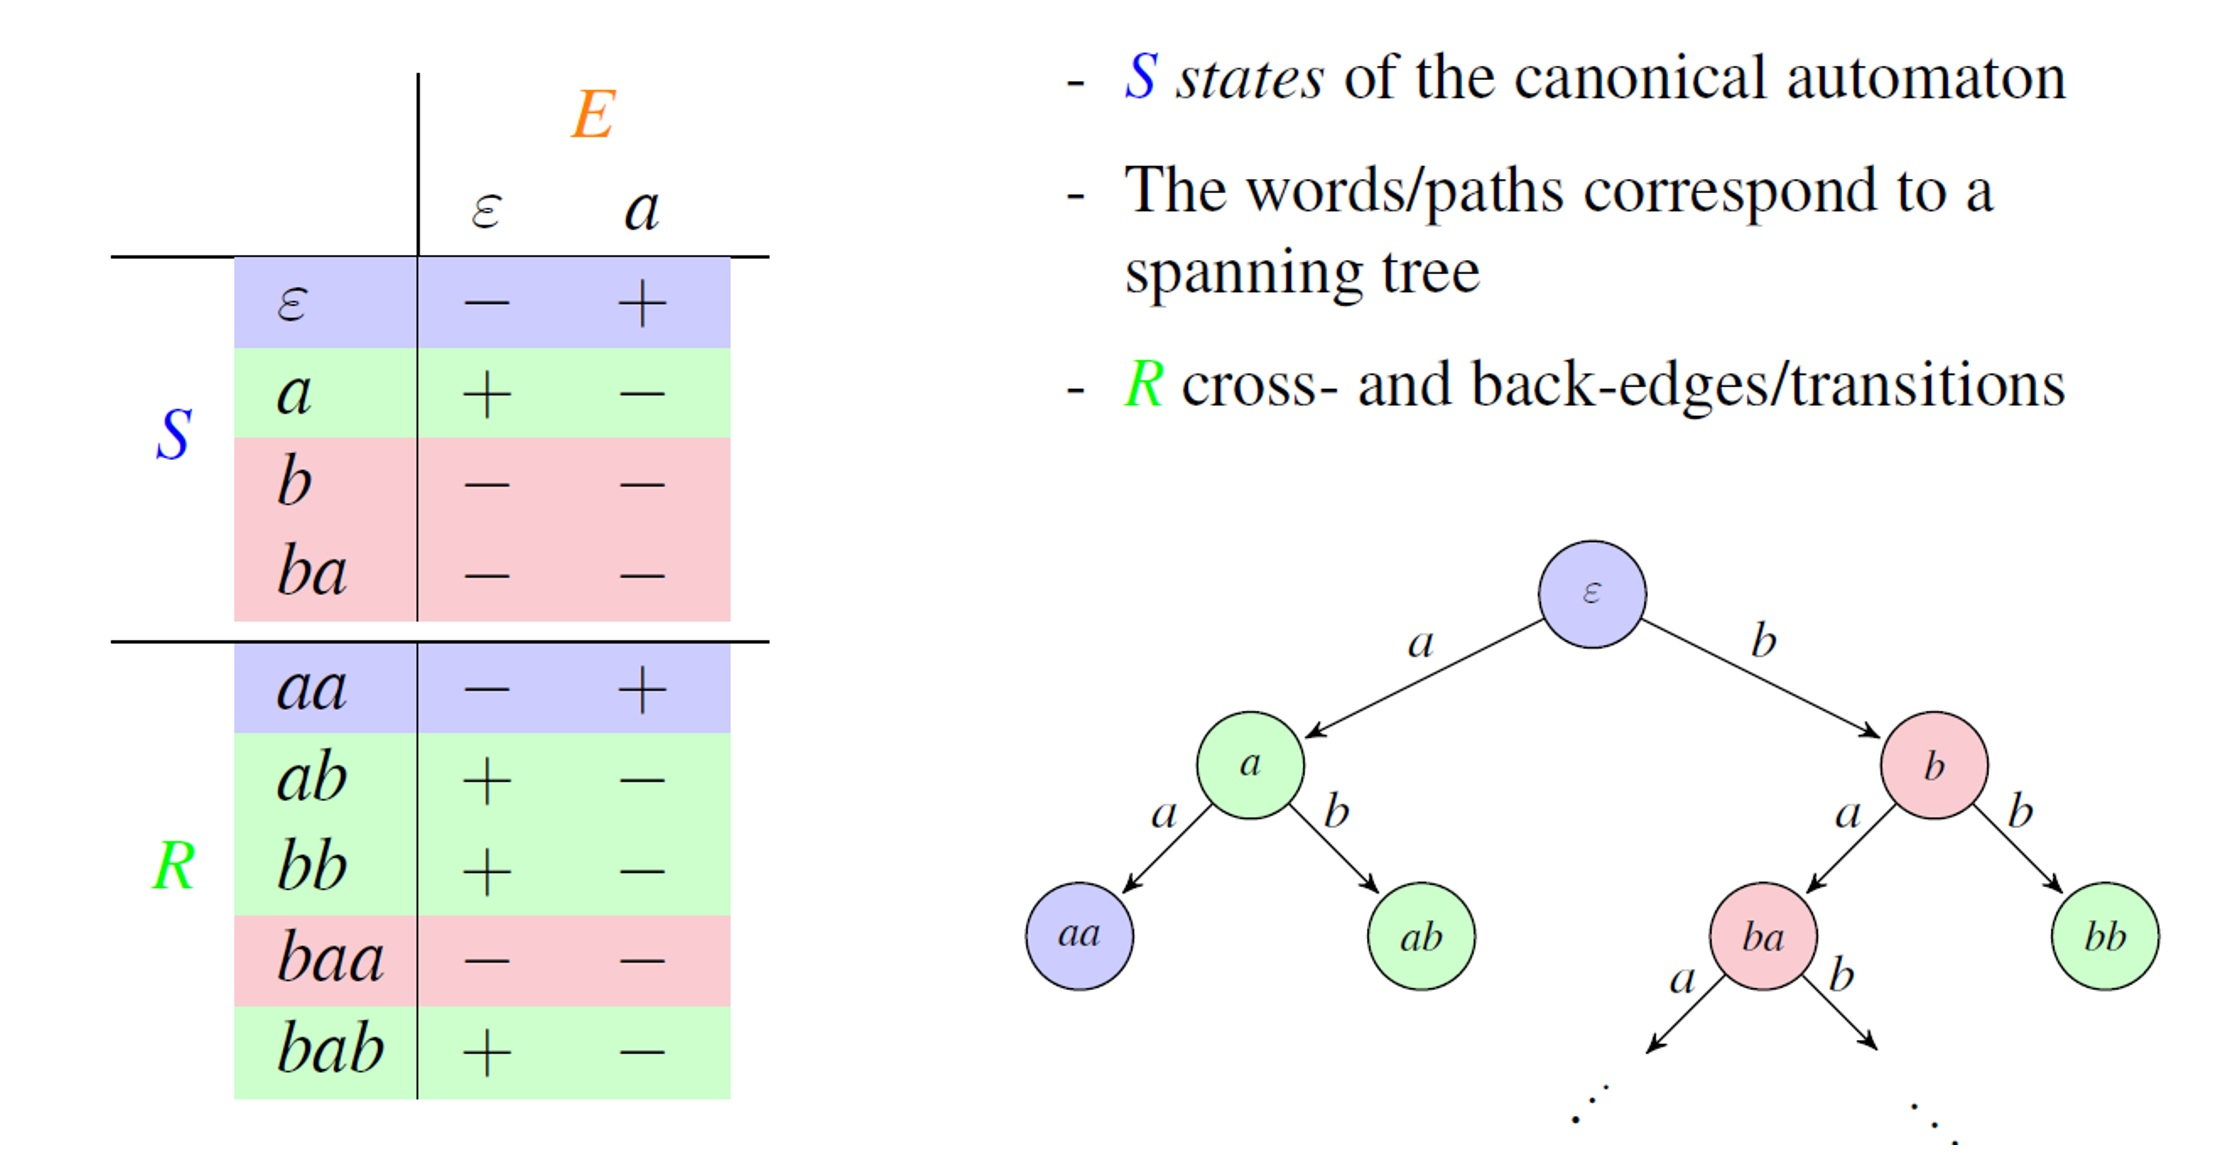
\includegraphics[width=\textwidth]{observationtable.jpg}
\end{center}

}

\frame{
\frametitle{Black Box Checking (Peled, Vardi \& Yannakakis)}

\begin{center}
 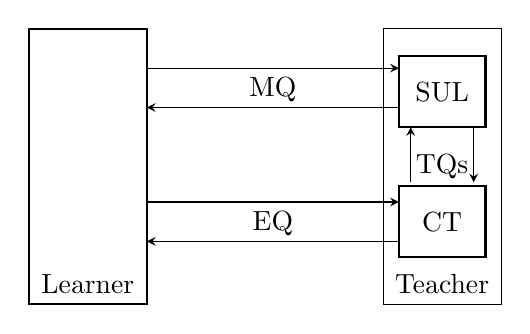
\begin{tikzpicture}[>=stealth]
            \draw [thick] (0,0) rectangle (1.5,3.5);
            \draw (4.5,0) rectangle (6,3.5) node[midway] {TQs};
            \draw [thick] (4.7,2.25) rectangle (5.8,3.15) node[midway] {SUL};
            \draw [thick] (4.7,0.6) rectangle (5.8,1.5) node[midway] {CT};
            \draw [->] (1.5,3) -- (4.7,3) node[midway,below] {MQ};
            \draw [<-] (1.5,2.5) -- (4.7,2.5);
            \draw [->] (1.5,1.3) -- (4.7,1.3) node[midway,below] {EQ};
            \draw [<-] (1.5,0.8) -- (4.7,0.8);
            \draw [->] (4.85,1.55) -- (4.85,2.25);
            \draw [<-] (5.65,1.55) -- (5.65,2.25);
            \node [below] at (0.75,0.5) {Learner};
            \node [below] at (5.25,0.5) {Teacher};
        \end{tikzpicture}
                \hspace{1 em}
        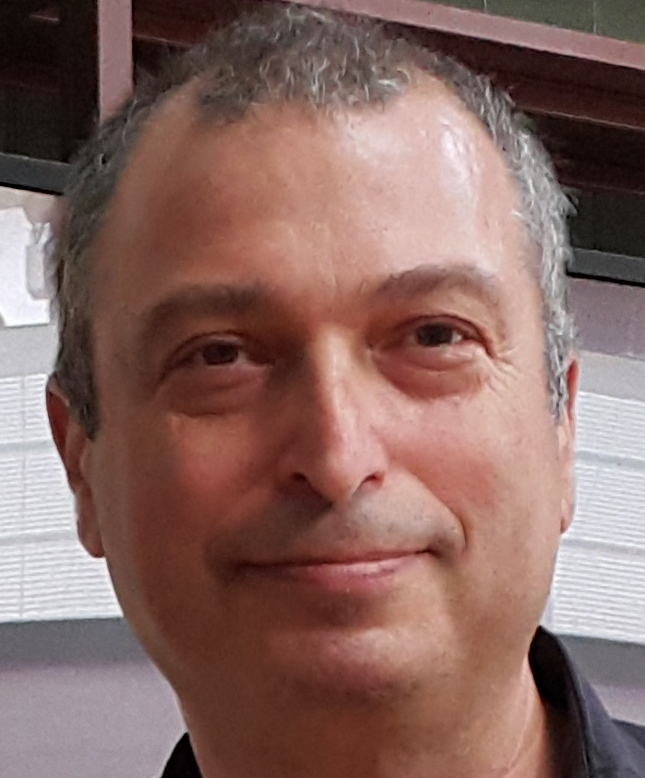
\includegraphics[width=1.2cm]{peled.jpg}
        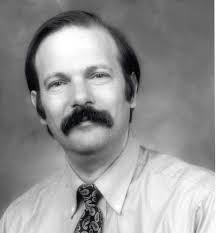
\includegraphics[width=1.35cm]{vardi.jpeg}
        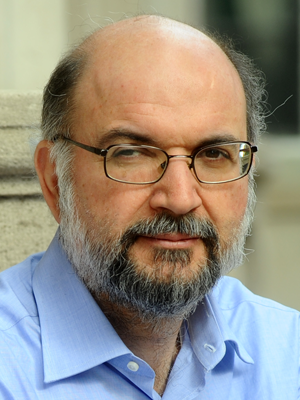
\includegraphics[width=1.1cm]{Yannakakis.png}
\end{center}
\red{Learner}: Formulate hypotheses\\
\red{Conformance Tester (CT)}: Test correctness hypotheses


\pause
\vspace{0.5em}
\red{Model learning and conformance testing two sides of same coin!}
}

\frame{
%\frametitle{LearnLib}

\begin{center}

\includegraphics[width=.7\textwidth]{LearnLib.jpg}
    \hspace{1 em}
        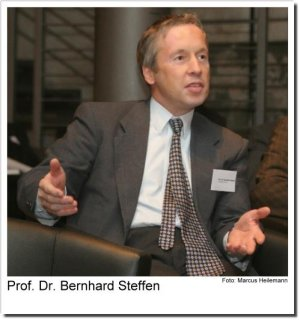
\includegraphics[width=2.5cm]{steffen.jpg}
\end{center}

Implements MAT framework for \red{DFAs}\  and \red{Mealy machines}
}

\section{Applications}

\frame{
	\frametitle{Our Research Method }
	
	\begin{center}
		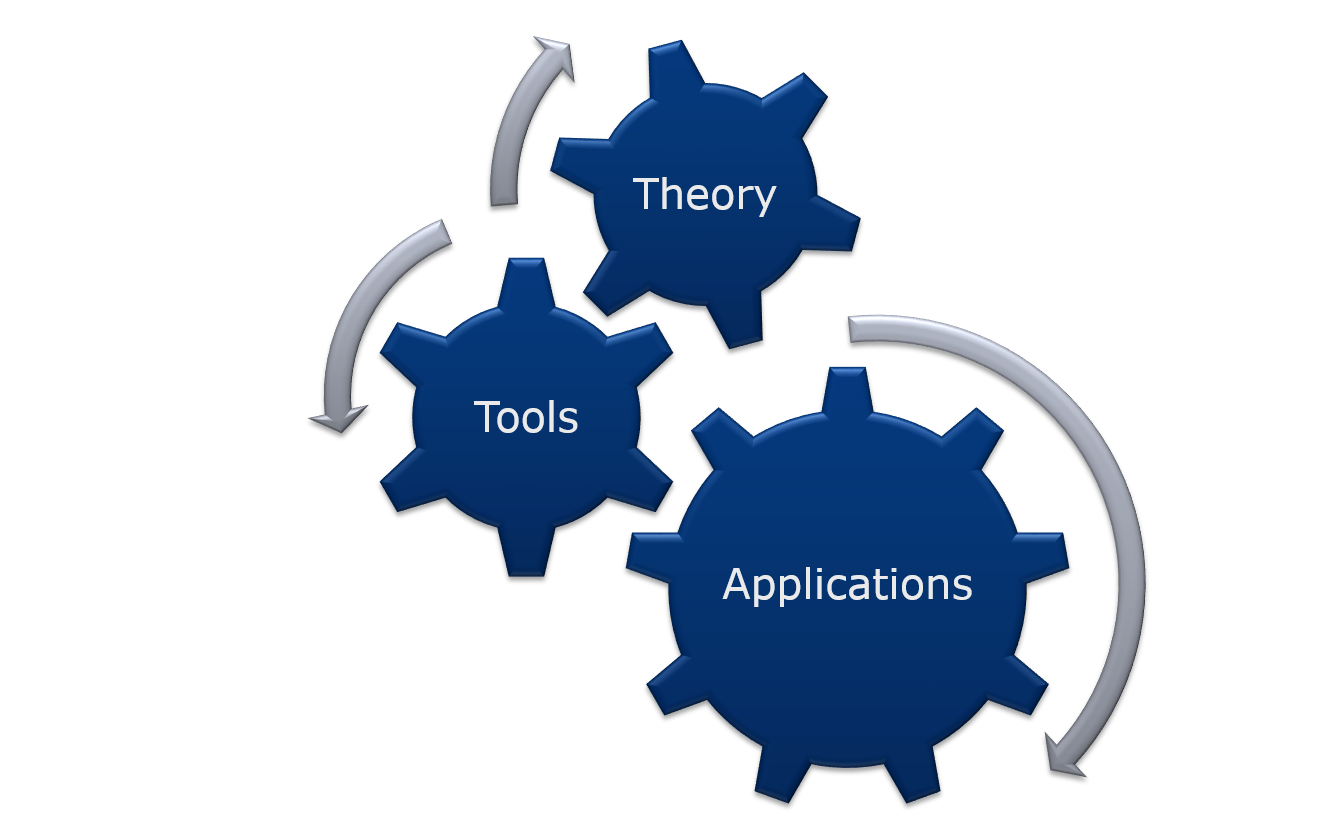
\includegraphics[width=.8\textwidth]{method.png}
	\end{center}
}

\frame{
	\frametitle{Engine Status Manager in Oc\'{e} Printer (ICFEM'15)}
	
	\begin{center}
		\includegraphics[width=.6\textwidth]{Oceprinter.png}
	\end{center}
	
	Can we learn interface models of realistic printer controllers?
	
	
}

\frame{
	\frametitle{Potential Applications Interface Models}
	
	\begin{center}
		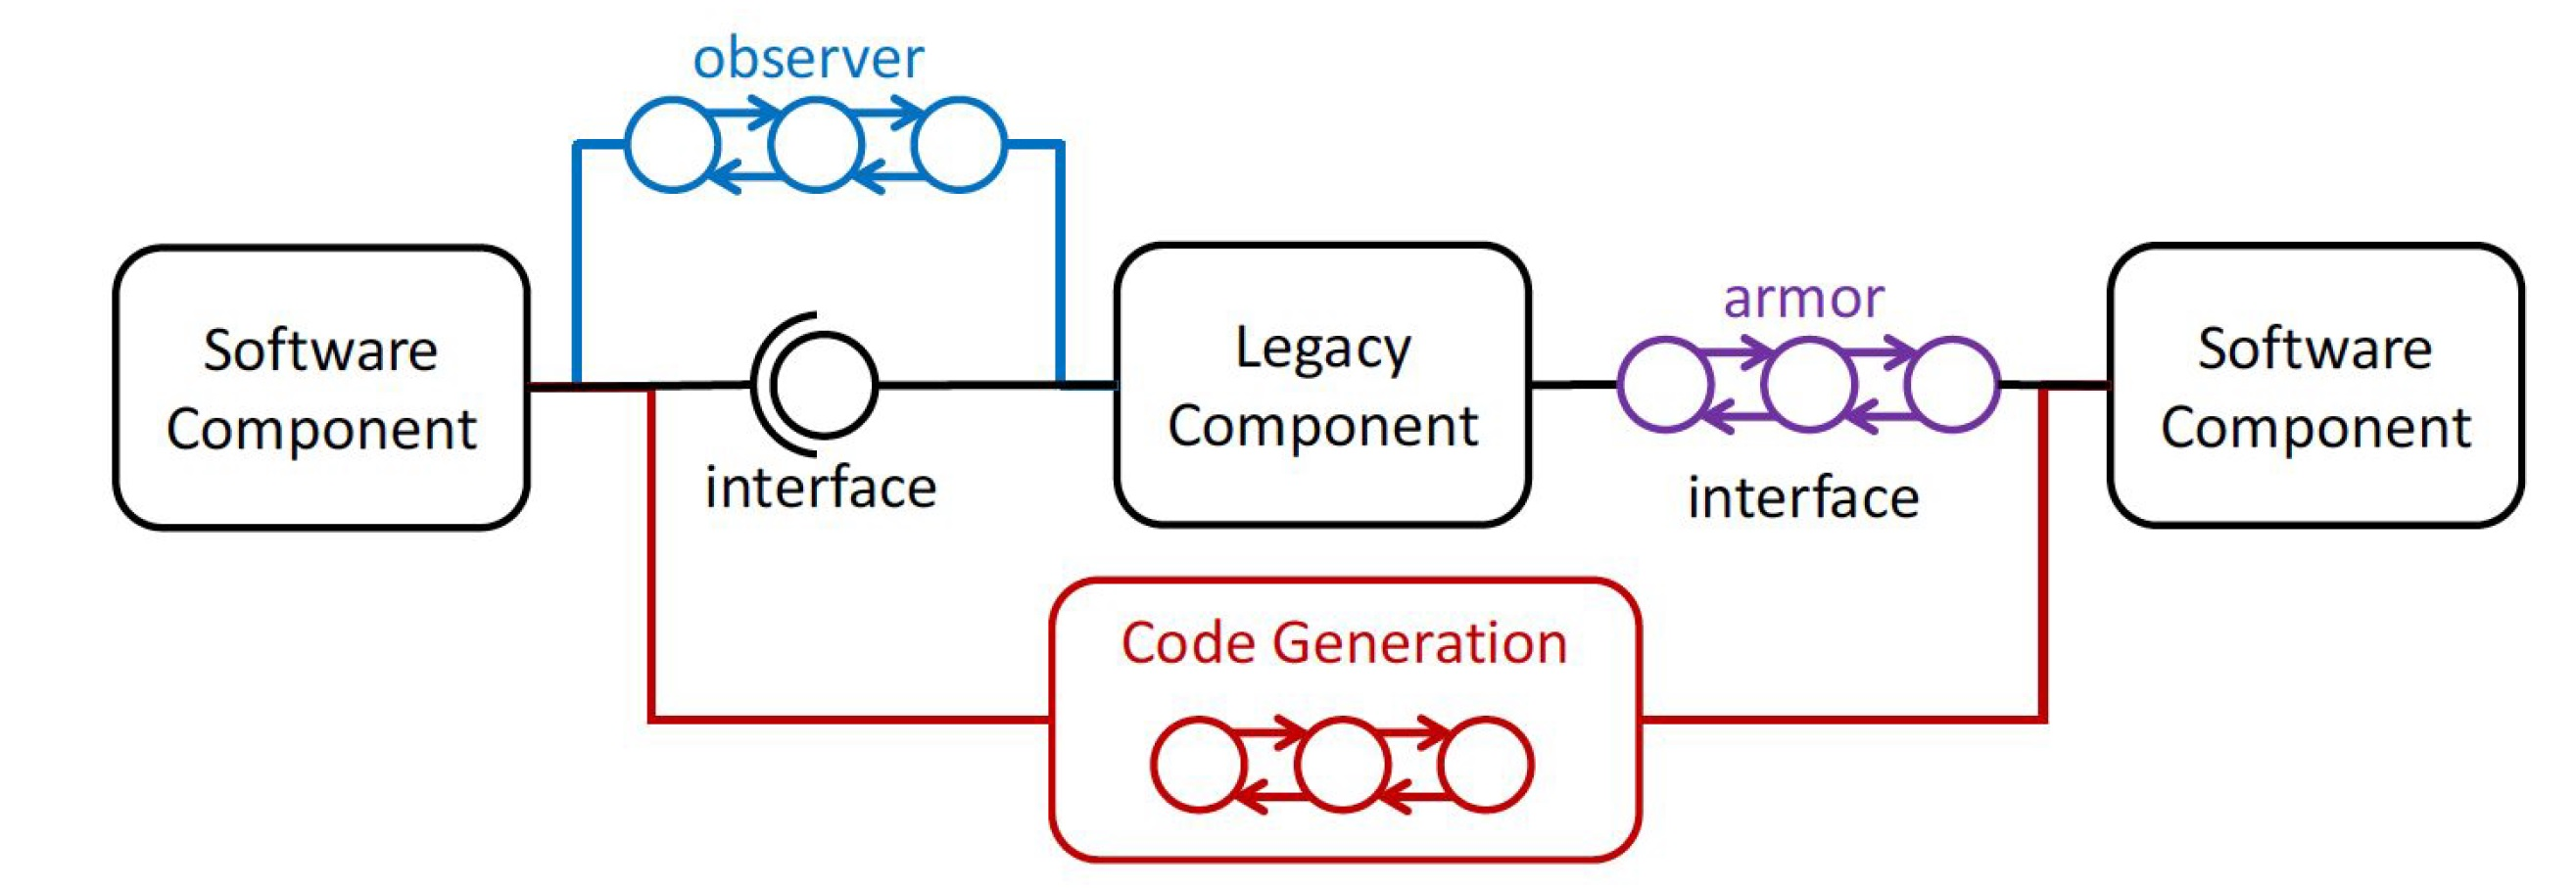
\includegraphics[width=\textwidth]{applicationsinterfacemodels}
	\end{center}
}

\frame{
	\frametitle{Conformance Testing Becomes Bottleneck!}
	
	No existing conformance testing methods (W, Wp, HSI, ADS, UIOv, P, H, SPY,..) was able to find counterexamples for some hypotheses models of the printer software. We had to develop a new \red{hybrid ADS}\  method, based on work of Lee \& Yannakakis.
	
	\begin{center}
		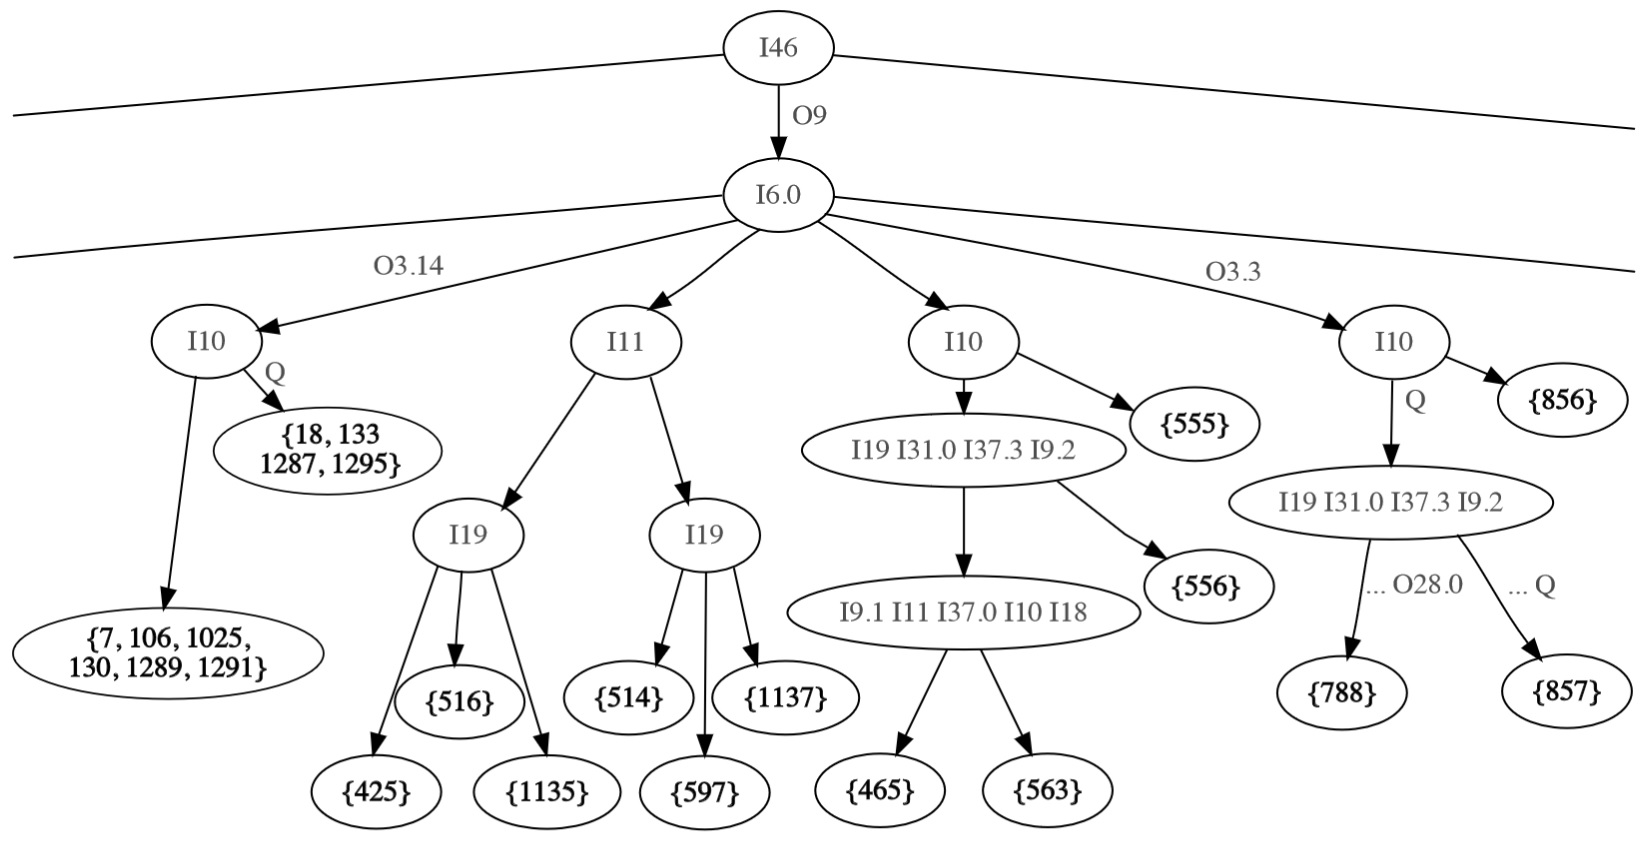
\includegraphics[width=.8\textwidth]{ADS.jpg}
	\end{center}
}


\frame{
	\frametitle{Mealy Machine for Engine Status Manager}
	\begin{center}	
		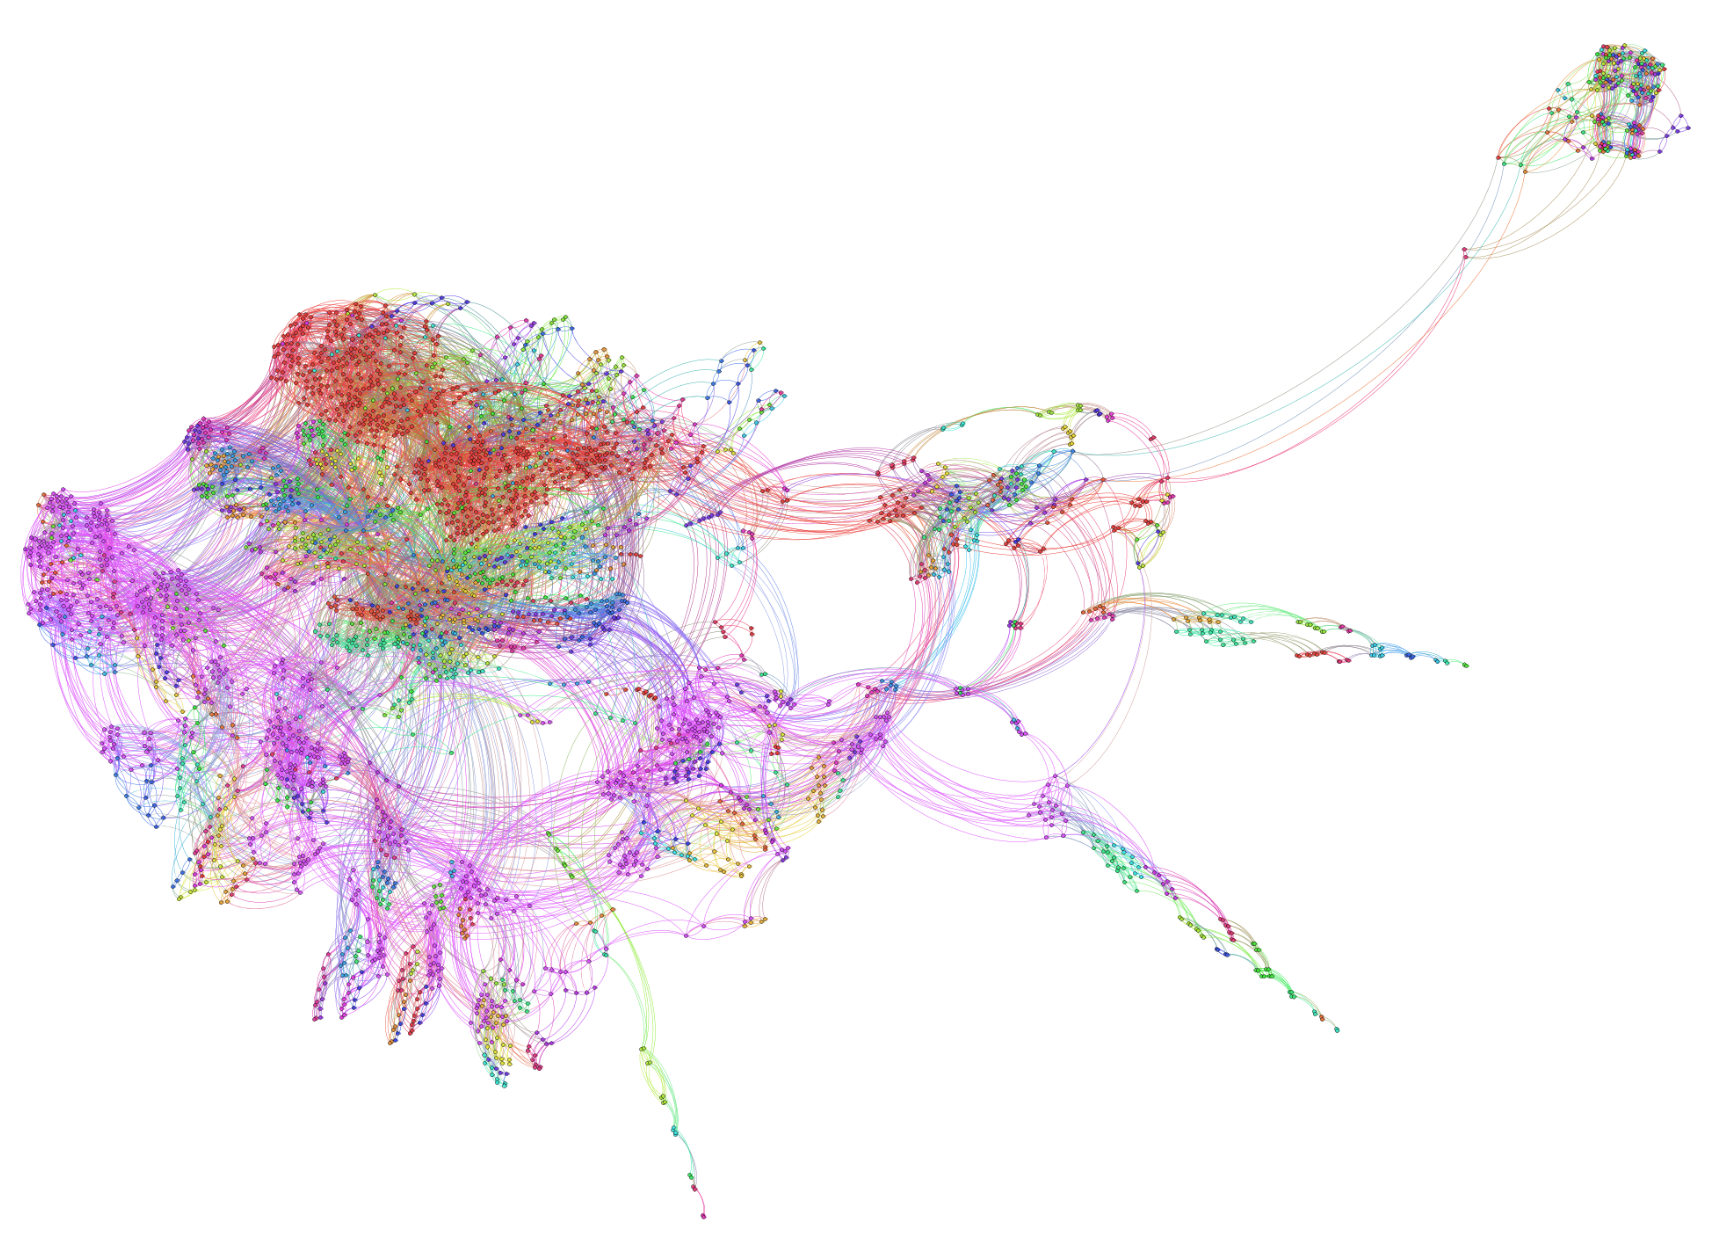
\includegraphics[width=0.8\textwidth]{ESM-manual.PNG}
	\end{center}
}

\frame{
	\frametitle{Power Control Service from Philips Healthcare (iFM'16)}
	
	\begin{center}
		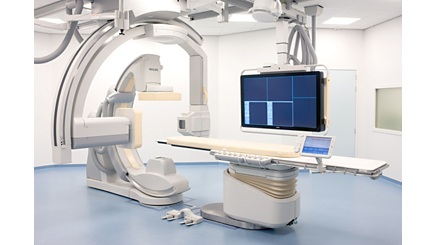
\includegraphics[width=.8\textwidth]{Xray.png}
	\end{center}
	
	Are legacy component and refactored implementation equivalent?
}

\frame{
	\frametitle{Refactoring Legacy Implementations}
	
	\begin{center}
		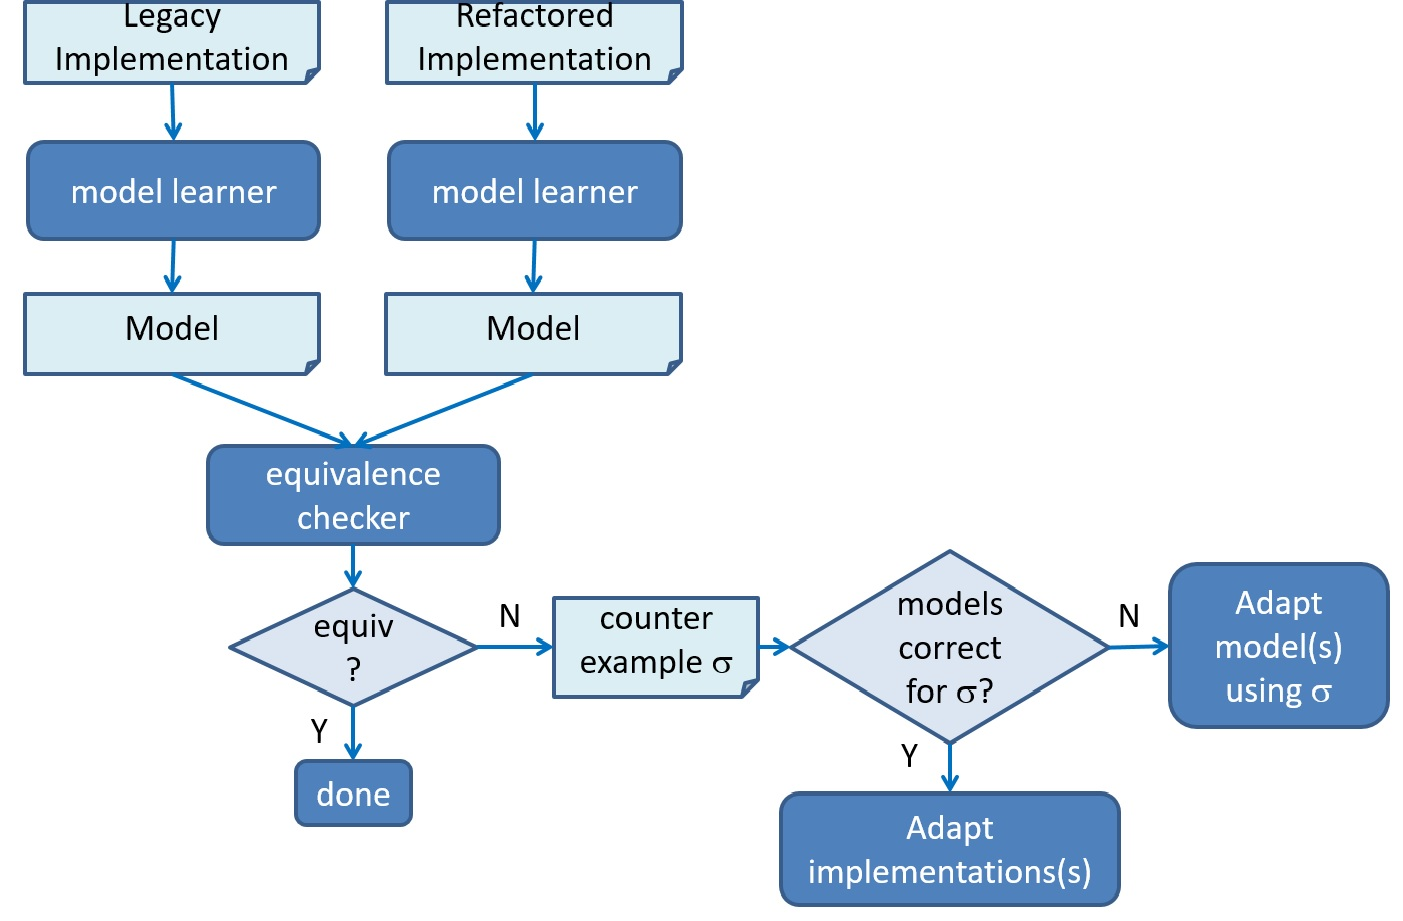
\includegraphics[width=.65\textwidth]{MethodeLegacy.jpg}
	\end{center}
	
	\pause
	\red{This approach allowed us to find several bugs in refactored implementations of power control service.}
	
	
}

\frame{
	\frametitle{ASML Twinscan}
	
	\begin{center}
		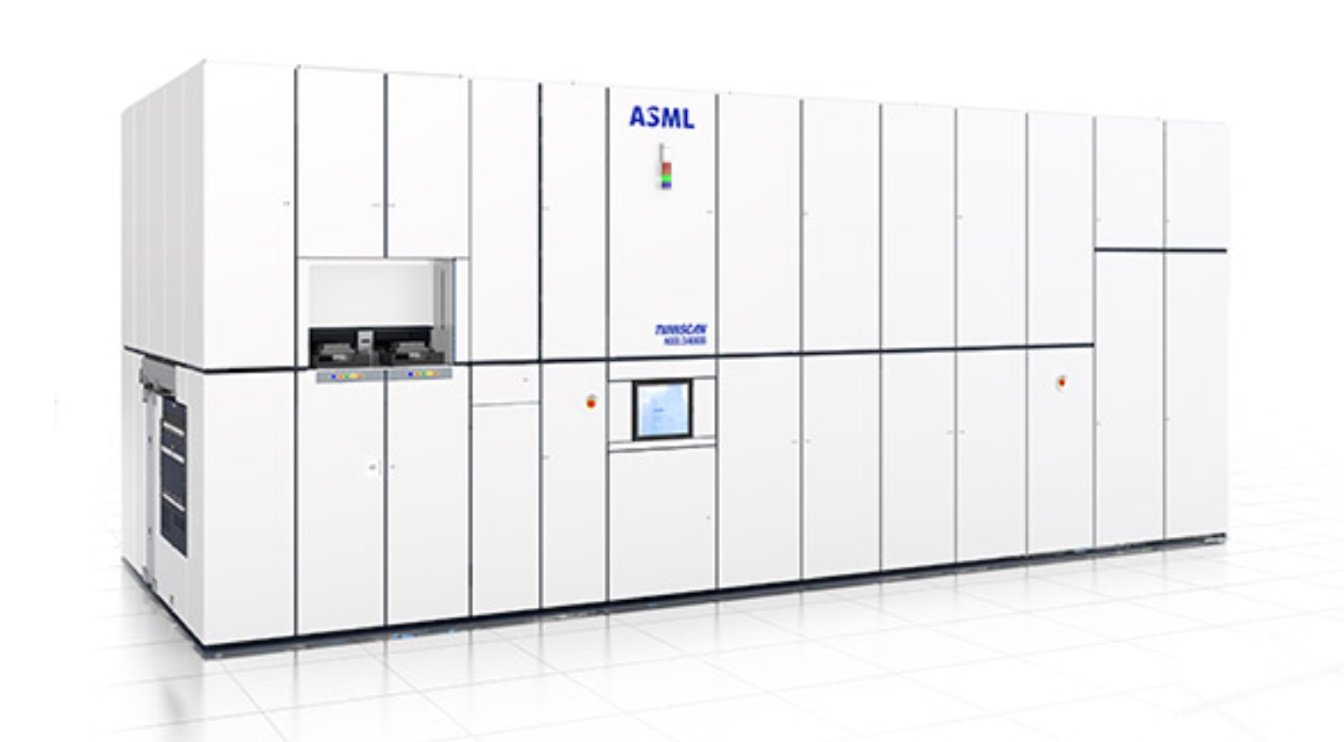
\includegraphics[width=\textwidth]{ASML-Feature.jpg}
	\end{center}
}

\frame{
	\frametitle{ASML Challenge}
	
	Can active automata learning be used to support refactoring of legacy software at ASML?
	
	\vspace{1 em}
	ASML machines run on legacy software. Recent components have been designed using model-based techniques. Can we learn those?
	
	\vspace{1 em}
	Can we learn the hundreds of design and interface models
	used for high level control of the wafer flow during lot operation?
	
	\pause
	\vspace{1 em}
	\red{$\Rightarrow$ RERS @ TOOLympics'19}
}

\frame{
	\frametitle{Results LearnLib on ASML Benchmarks}
	
	\begin{center}
		\includegraphics[width=0.8\textwidth]{ASMLBenchmarks.jpg}
	\end{center}
	
}


\frame{
\frametitle{A Theory of Mappers (FMSD, 2015)}

\begin{center}
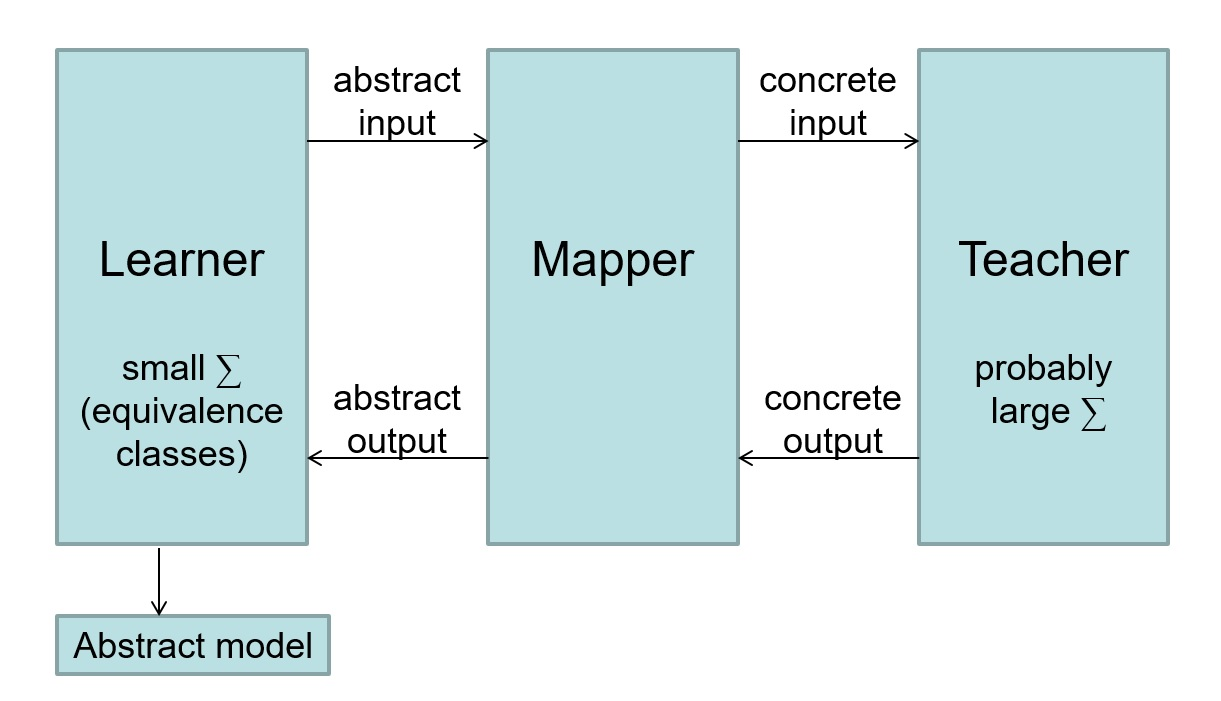
\includegraphics[width=.9\textwidth]{mappers.jpg}
\end{center}
}

%\frame{
%\frametitle{A Theory of Mappers (cnt)}
%
%Formally, a mapper can be viewed as a transducer (deterministic Mealy machine). A mapper ${\cal A}$ induces an \red{abstraction operation\ } $\alpha_{\cal A}$ and a \red{concretization\ } operator $\gamma_{\cal A}$.
%
%\begin{theorem}
%Suppose $\alpha_{\cal A}({\cal M})$ has no transitions with output $\perp$.
%For a mapper ${\cal A}$ and nondeterministic Mealy machines ${\cal M}$ and ${\cal H}$,
%$\alpha_{\cal A}({\cal M}) \leq {\cal H}$ iff
%${\cal M} \leq \gamma_{\cal A}({\cal H})$.  \tiny{(modulo a minor technical condition)}
%\end{theorem}
%}


%\frame{
%\frametitle{EMV Protocol (Aarts et al, 2013)}
%
%\begin{columns}
%\begin{column}{0.5\textwidth}
%    \begin{center}
%     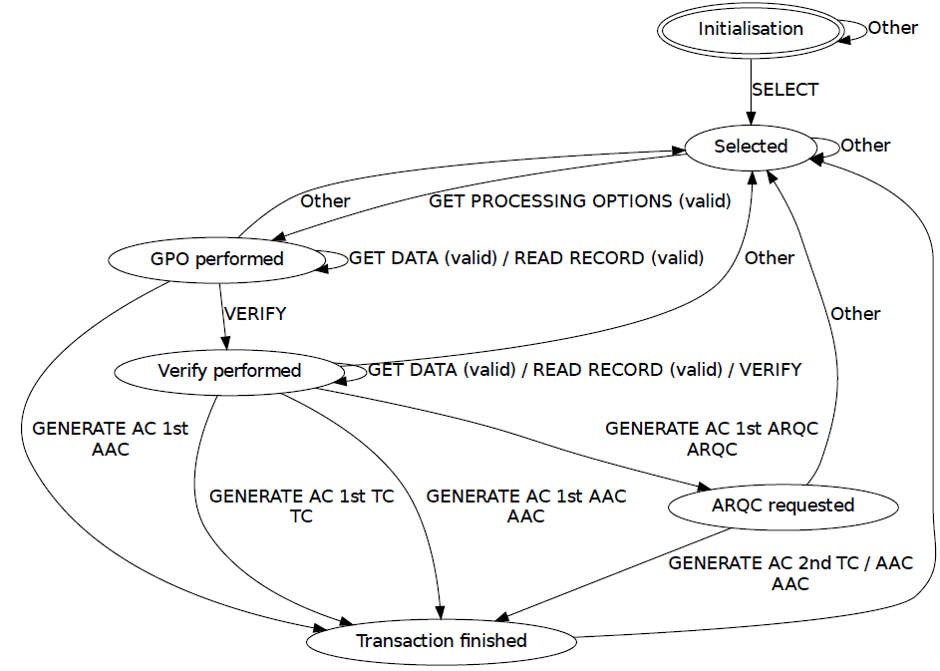
\includegraphics[width=\textwidth]{EMV.png}
%     \end{center}
%\end{column}
%\begin{column}{0.5\textwidth}
%{\small
%\begin{itemize}
%\item 
%EMV = Europay/Mastercard/Visa
%\item
%Compatibility between smartcards and terminals 
%\item
%SEPA requires EMV compliance
%\item
%EMV standard has $>$700 pages
%\item
%Learning took at most 1500 membership queries, less than 30 minutes
%\item
%Useful for fingerprinting cards
%\end{itemize}
%}
%\end{column}
%\end{columns}
%}
%\frame{
%\frametitle{E.dentifier2 (WOOT'14)}
%\begin{center}
%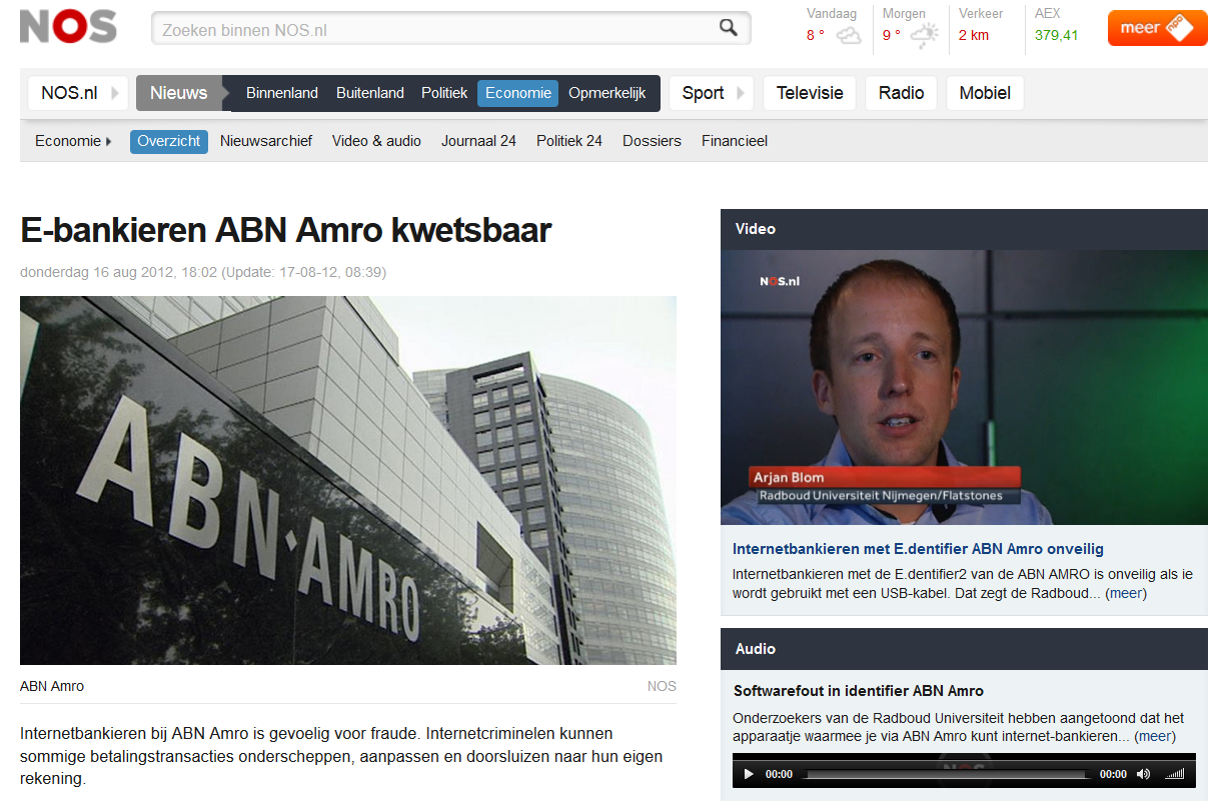
\includegraphics[width=.8\textwidth]{nosedentifier.png}
%\end{center}
%}

%
%\frame{
%	\frametitle{Learning a Model of the E.dentifier2}
%	
%	\begin{columns}
%		\begin{column}{0.5\textwidth}
%			\begin{center}
%				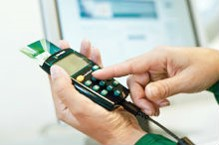
\includegraphics[width=0.9\textwidth]{edentifier}
%			\end{center}
%		\end{column}
%		\begin{column}{0.5\textwidth}
%			\begin{center}
%				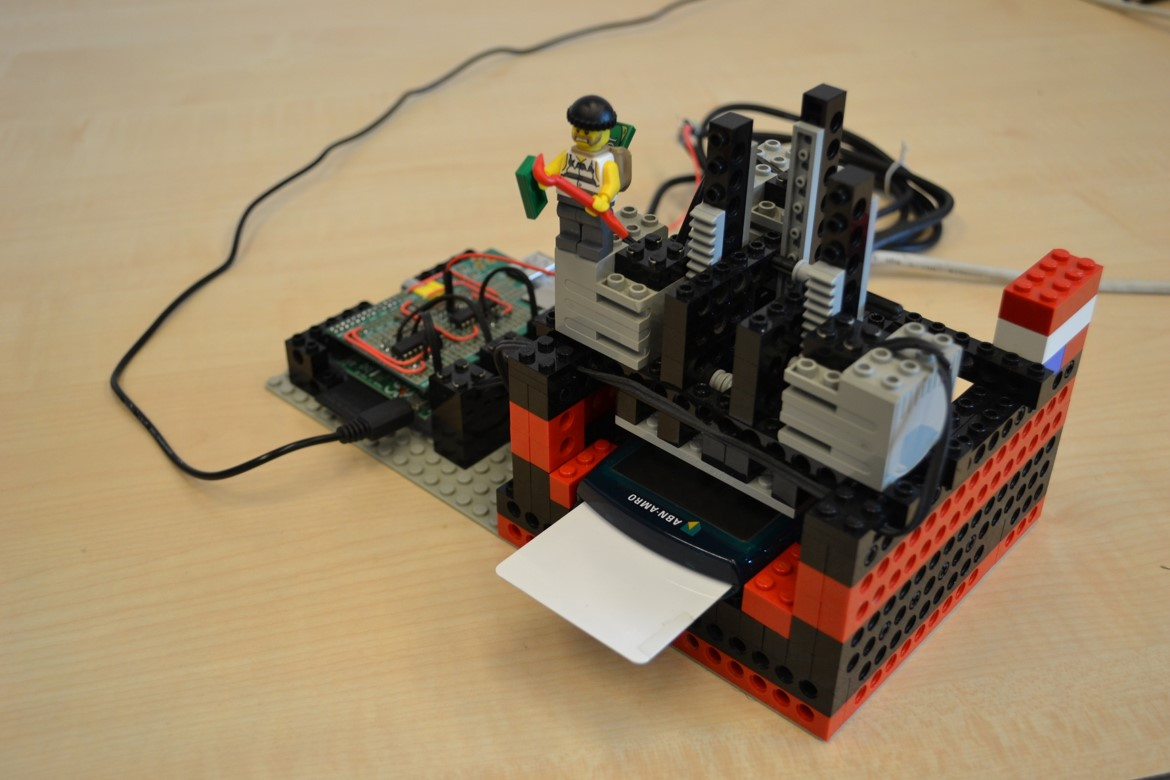
\includegraphics[width=0.9\textwidth]{legorobot}
%			\end{center}
%		\end{column}
%	\end{columns}
%}
%\frame{
%\frametitle{State Machines for Old and New E.dentifier2}
%\begin{center}
%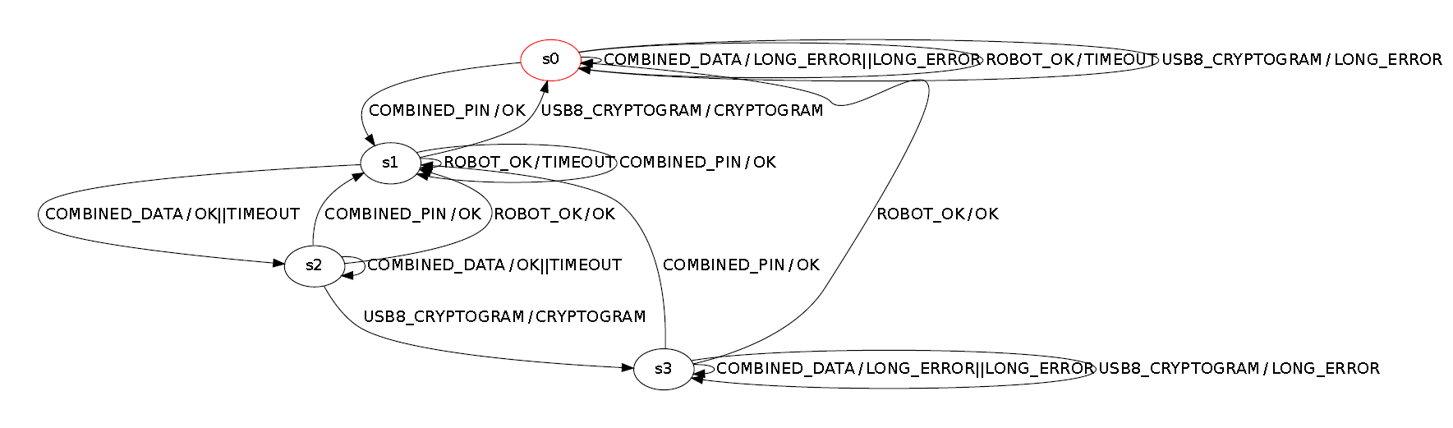
\includegraphics[width=.9\textwidth]{oldedentifier.png}
%
%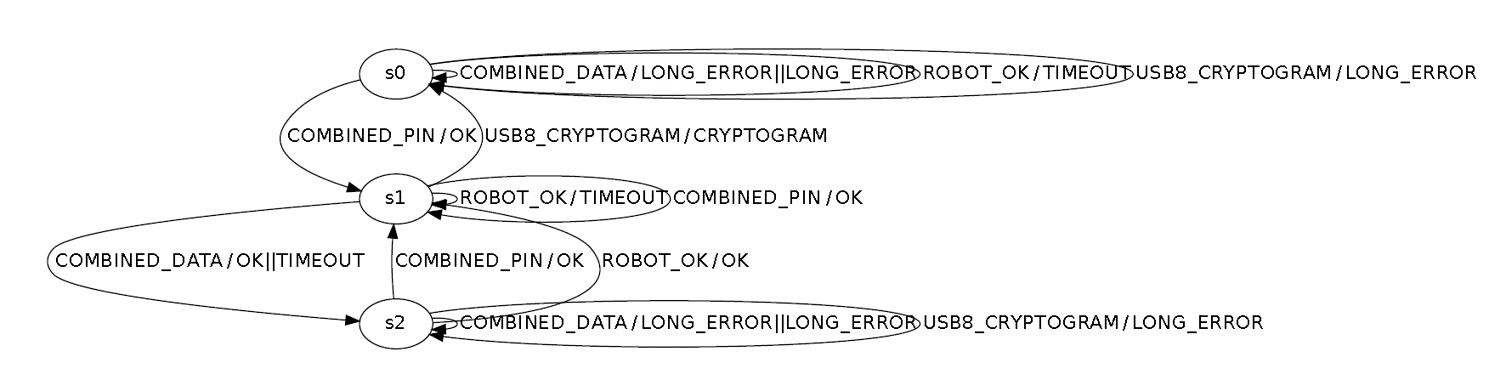
\includegraphics[width=.9\textwidth]{newedentifier.png}
%\end{center}
%}

\frame{
\frametitle{Bugs in Protocol Implementations}

\begin{columns}
\begin{column}{0.5\textwidth}  %%<--- here
    \begin{center}
     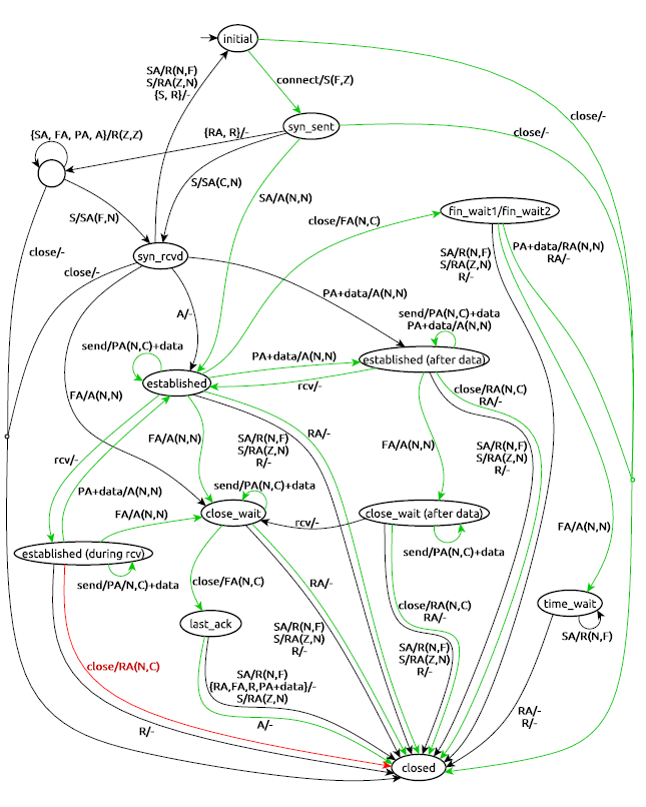
\includegraphics[width=0.9\textwidth]{TCPbug.png}
     \end{center}
\end{column}
\begin{column}{0.5\textwidth}
Standard violations found in implementations of major protocols: 
\begin{itemize}
\item
\blue{TLS}\  (Usenix Security'15)
\item 
\blue{TCP}\  (CAV'16)
\item
\blue{SSH}\  (Spin'17)
\end{itemize}
%
\pause
\red{These findings led to bug fixes in implementations.}
\end{column}
\end{columns}

}

\frame{
\frametitle{Learned Model for SSH Implementation}

\begin{center}
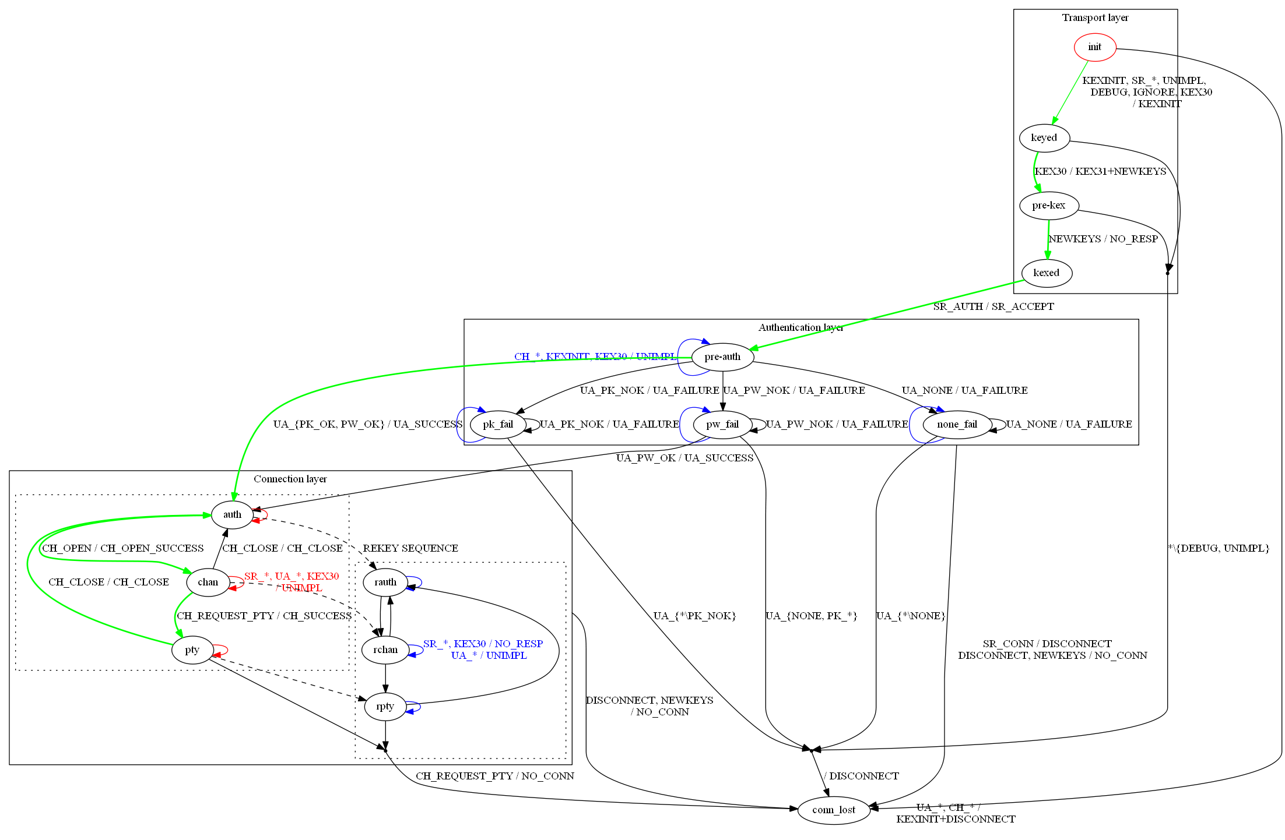
\includegraphics[width=\textwidth]{sshbug.png}
\end{center}
}
\frame{
\frametitle{SSH Model Checking Results}

\begin{center}
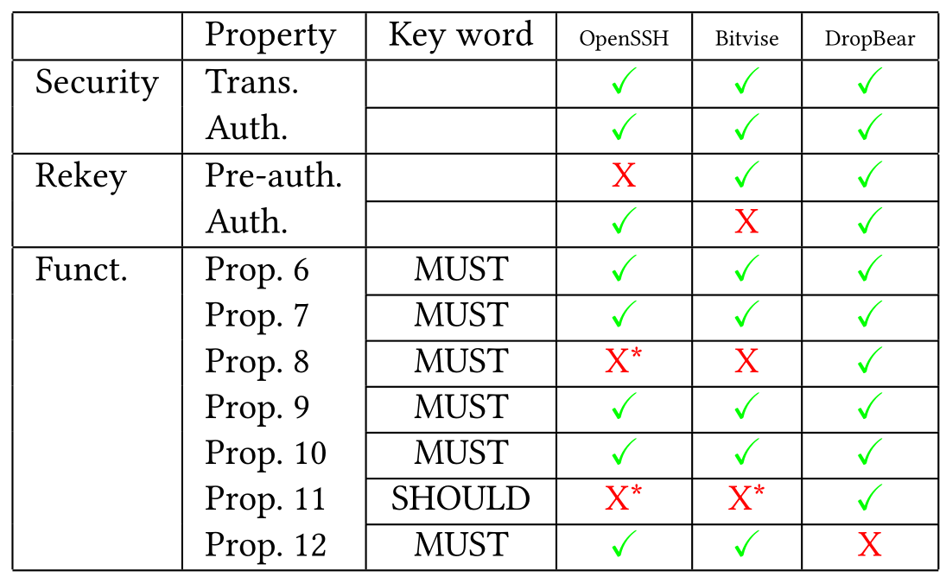
\includegraphics[width=\textwidth]{sshresults.png}
\end{center}
}

\frame{
\frametitle{Other Protocol Case Studies}
\begin{itemize}
	\item
	Biometric Passport
	\item
	EMV Protocol
\item
Session Initiation Protocol (SIP)
\item
Message Queuing Telemetry Transport (MQTT) protocol
\item
Quick UDP Internet Connections (QUIC) protocol
\item
WiFi
\item
IEC 60870-5-104 protocol
\item
...
\end{itemize}
}

\frame{
\frametitle{Fingerprinting TLS Implementations}

There are many different TLS implementations.  How can we figure out to which implementation we are talking?

Our approach:
\begin{itemize}
	\item 
	Learn state machine models of hundreds of TLS implementations
	\item
	Consider disjoint union of these state machines and add reset transitions
	\item
	Use algorithm of Lee \& Yannakakis to compute adaptive distinguishing sequence
\end{itemize}

\green{(joint work with Erwin Janssen and Joeri de Ruiter, SIDN)}
}

\frame{
\frametitle{Lorentz Workshop}

\begin{columns}
\begin{column}{0.5\textwidth}  %%<--- here
    \begin{center}
     \includegraphics[width=0.9\textwidth]{lorentz.jpg}
     \end{center}
\end{column}
\begin{column}{0.5\textwidth}
Participants from automata learning, model-based testing, cryptography, and security protocol implementation. 

\vspace{0.5em}
Working groups on e.g.,
   \begin{itemize}
   \item 
   WiFi
   \item
   side channels in TLS
   \item
   LTE
   \end{itemize}
\end{column}
\end{columns}
}





\section{From Black Box to Grey Box Learning}
%\frame{
%\frametitle{Benchmark Wiki \url{automata.cs.ru.nl}}
%
%\begin{center}
%
\includegraphics[width=.9\textwidth]{automatawiki.jpg}
%\end{center}
%}


%\frame{
%\frametitle{Benchmark Wiki \url{automata.cs.ru.nl}}
%
%\begin{center}
%
\includegraphics[width=.9\textwidth]{benchmarks.jpg}
%\end{center}
%}


%\frame{
%\frametitle{Benchmark Wiki: Supported Automata Frameworks}
%
%\begin{center}
%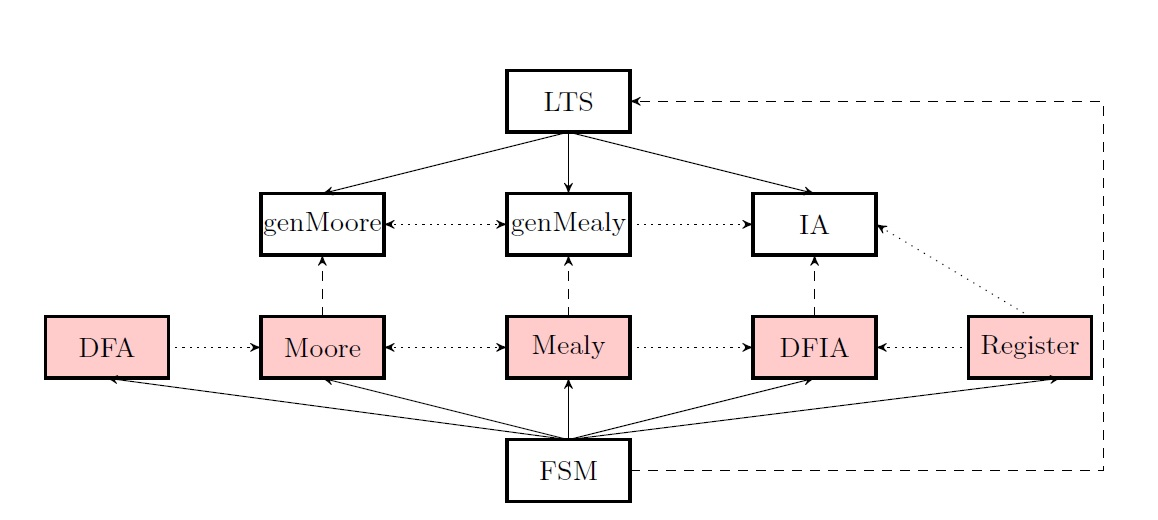
\includegraphics[width=\textwidth]{automataframeworks.jpg}
%\end{center}
%}


%\frame{
%\frametitle{Automata Wiki: Most Benchmarks are not that Big}
%
%\begin{center}
%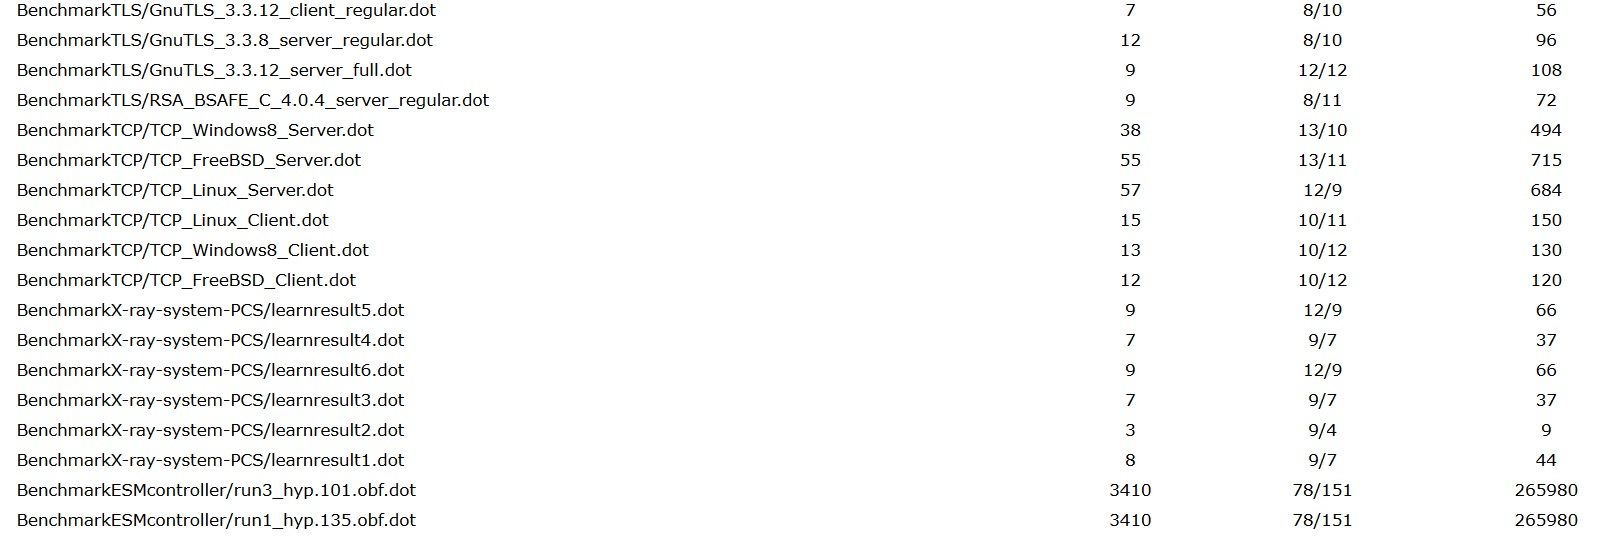
\includegraphics[width=\textwidth]{benchmarksize.jpg}
%\end{center}
%}


%\frame{
%	\frametitle{Learning Product Automata (Moerman, ICGI'18)}
%	
%	Consider a Moore machine with outputs $O_1 \times O_2$
%	
%	\begin{center}
%		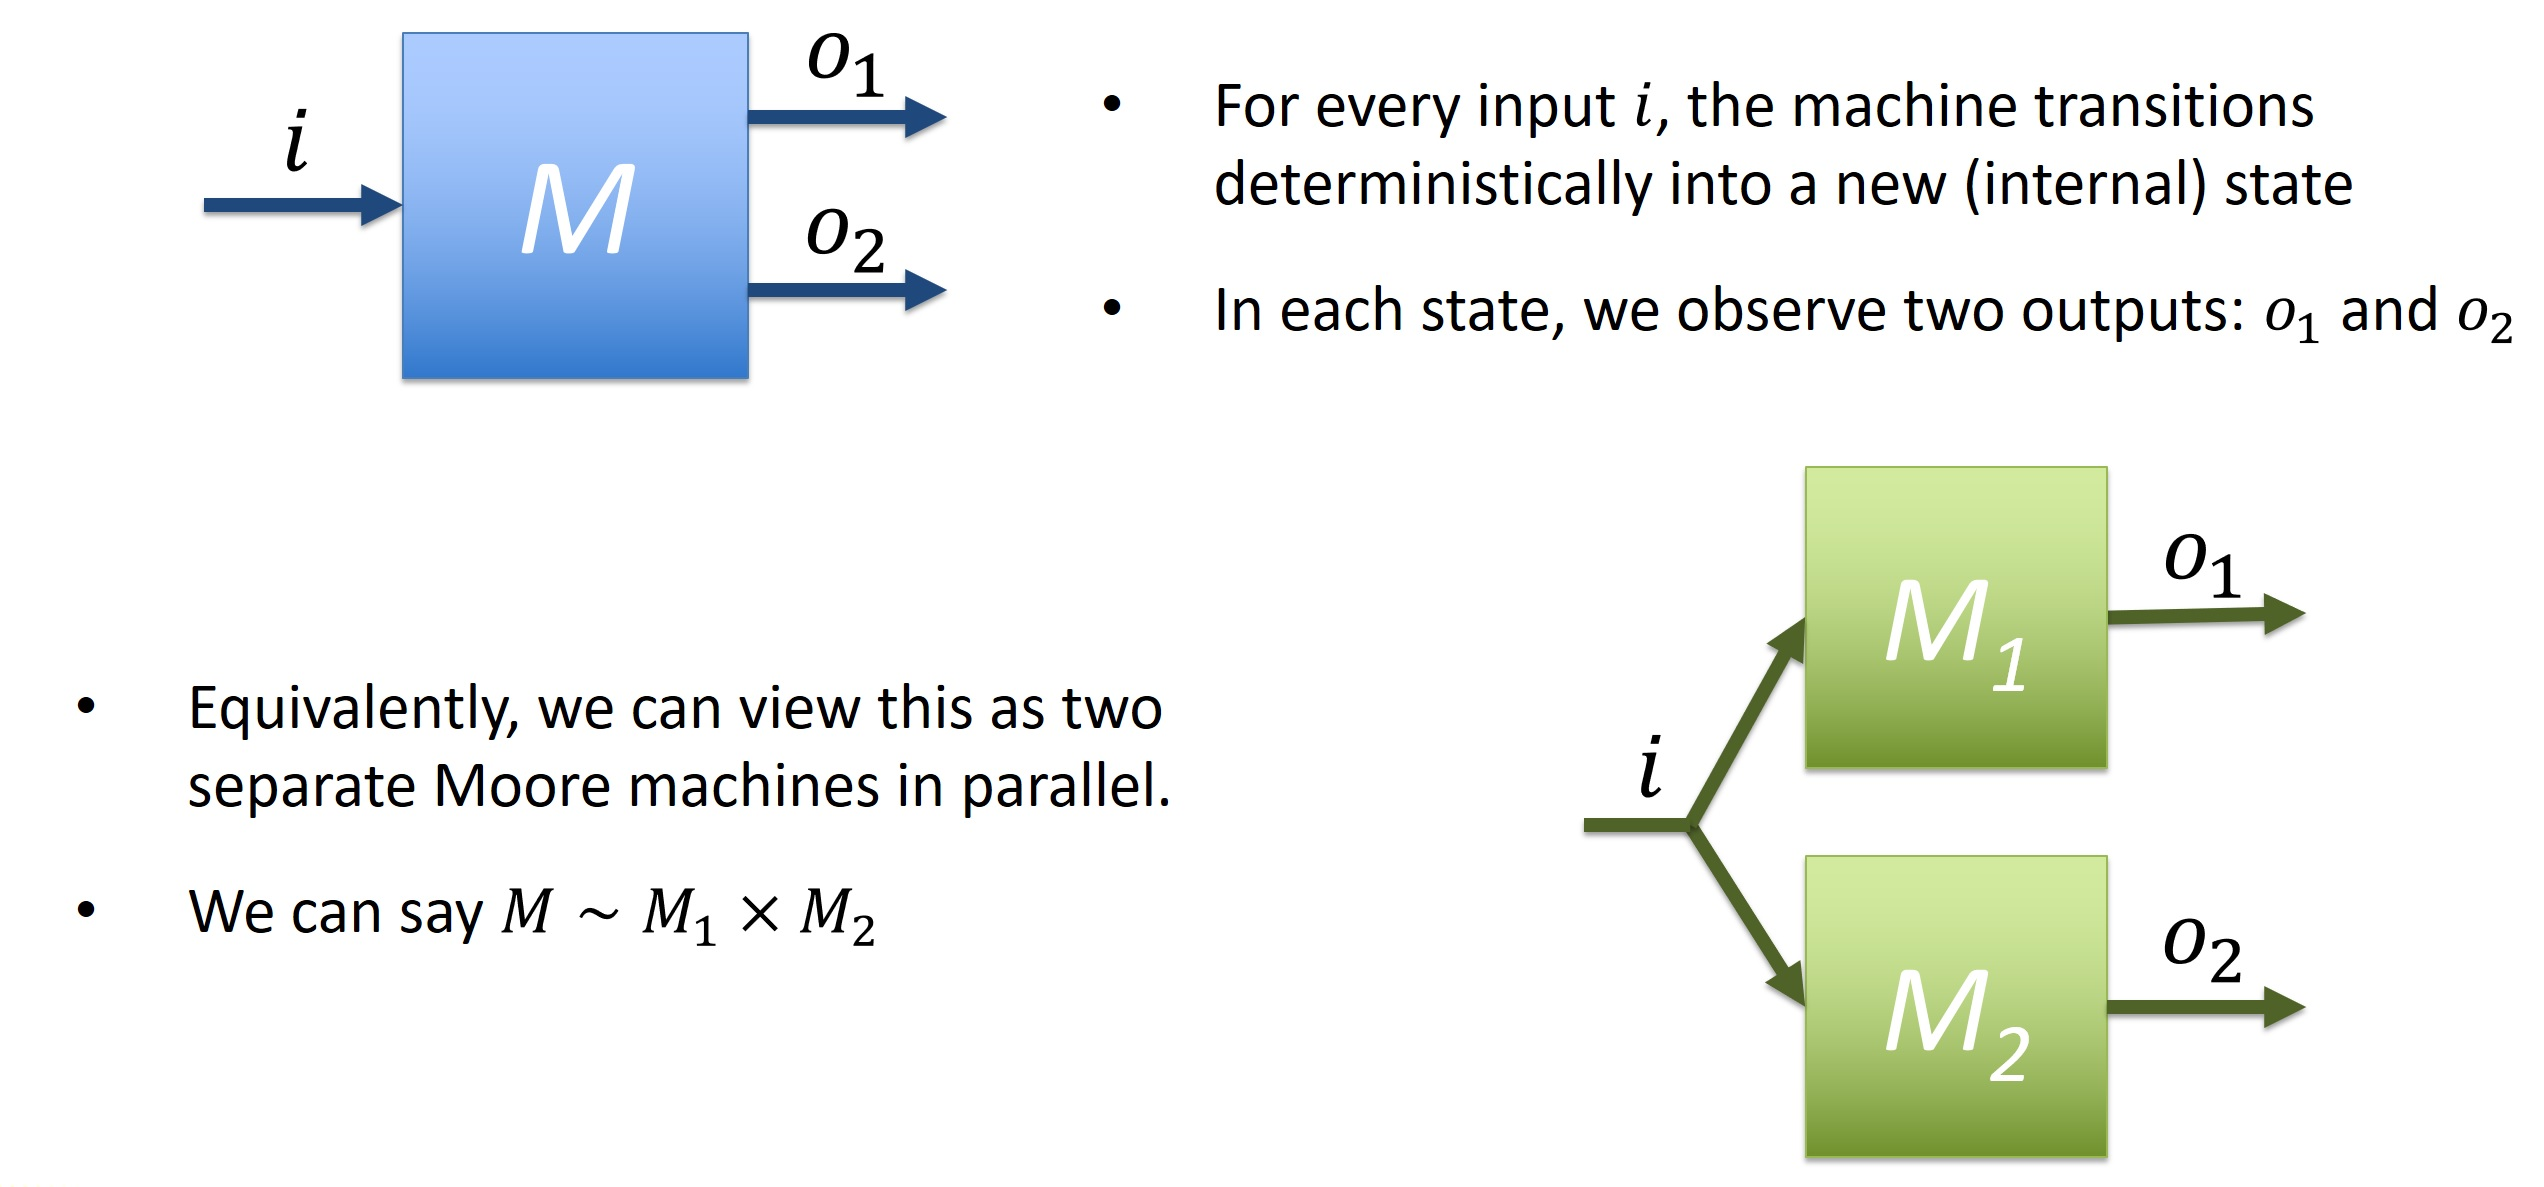
\includegraphics[width=\textwidth]{productautomata.jpg}
%	\end{center}
%}
%
%\frame{
%	\frametitle{An Example from Rivest \& Schapire}
%		
%	\begin{center}
%		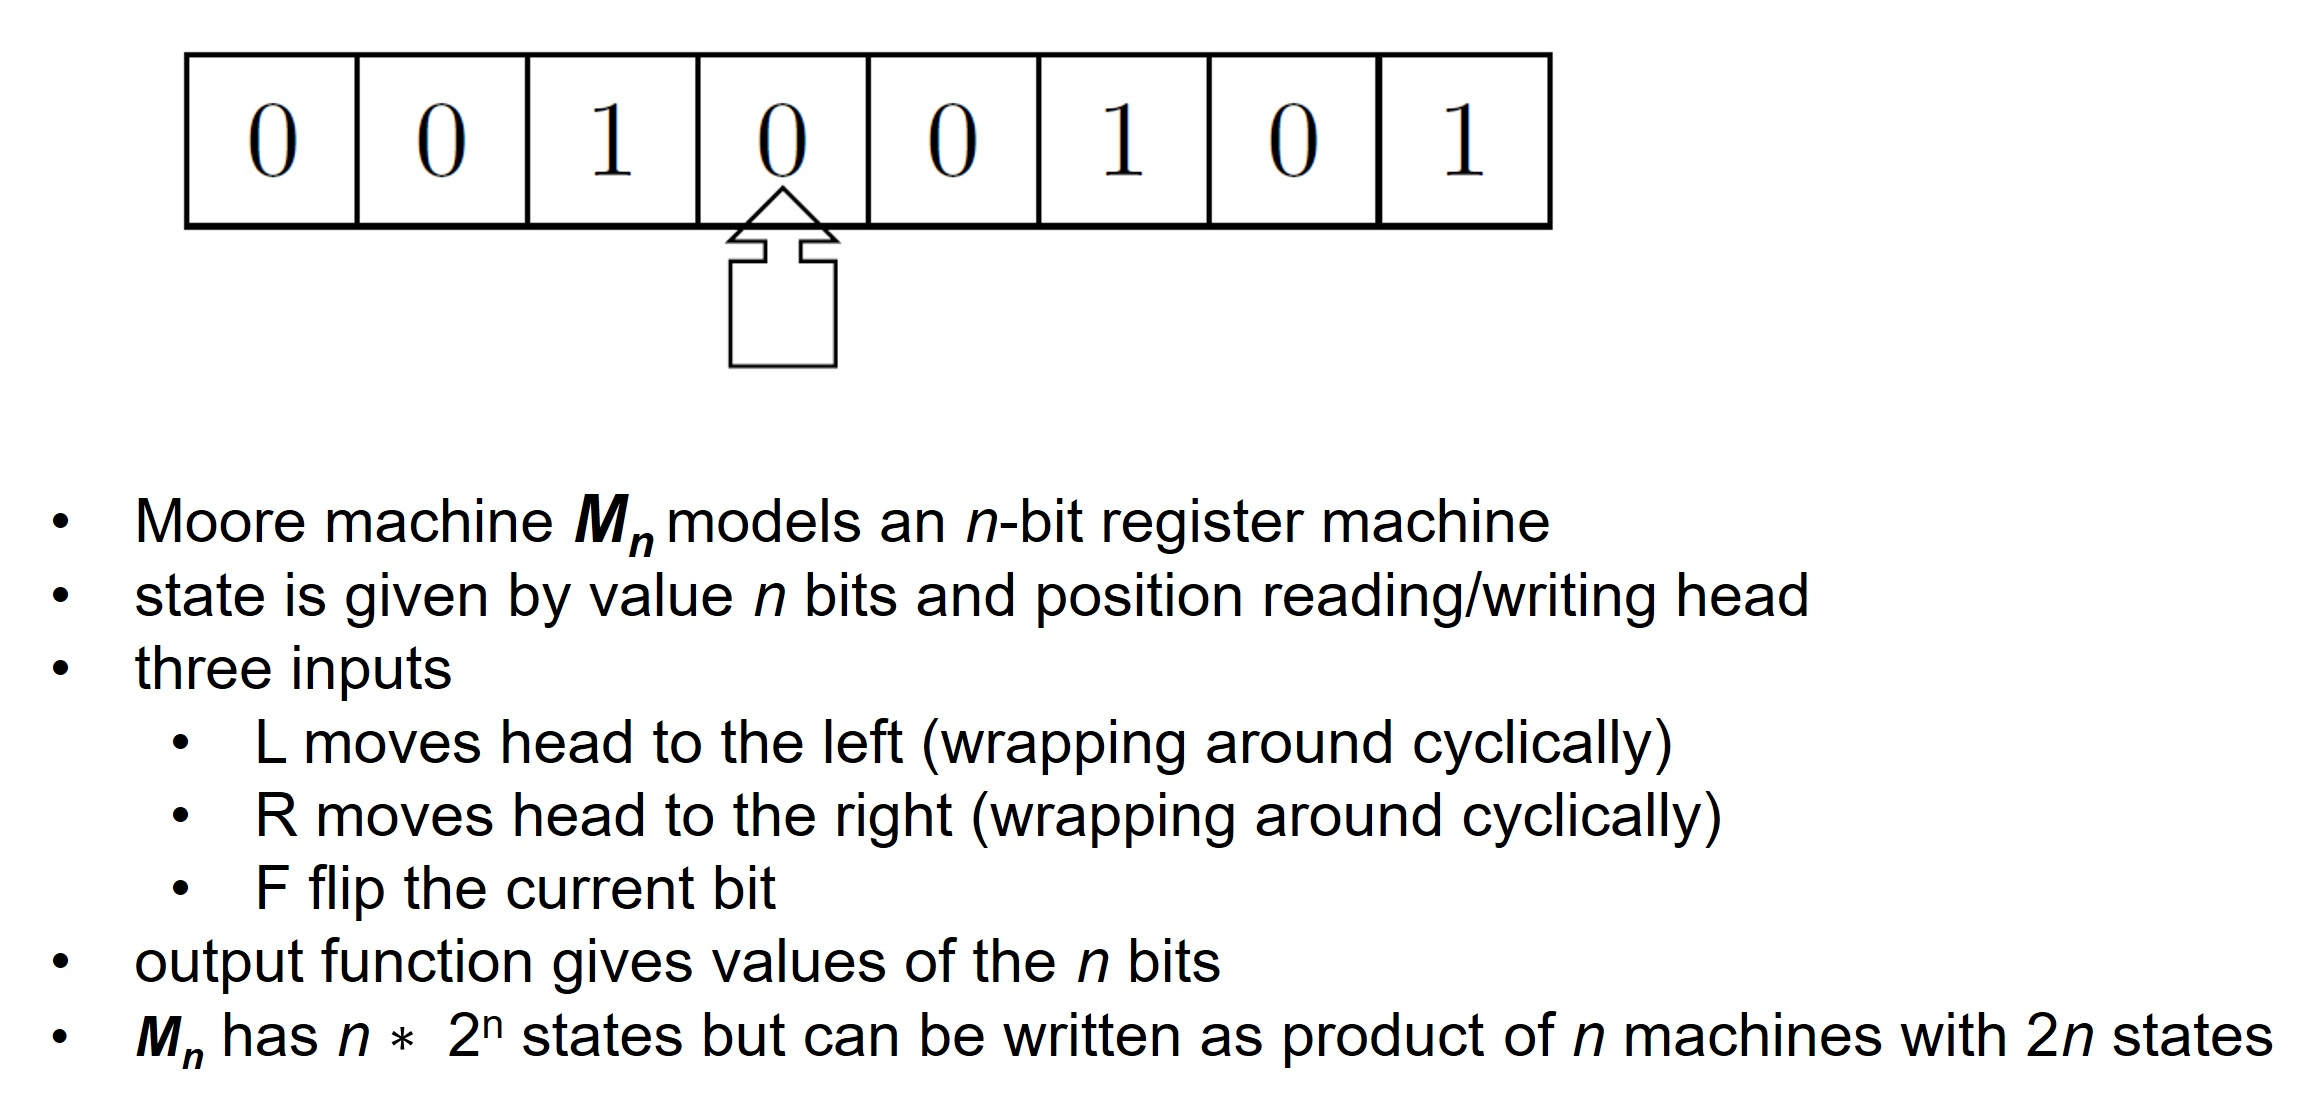
\includegraphics[width=\textwidth]{rivestschapire.jpg}
%	\end{center}
%}
%
%\frame{
%	\frametitle{Experimental Evaluation}
%	
%	\begin{center}
%		\includegraphics[width=\textwidth]{experimentsproduct.jpg}
%	\end{center}
%}

\frame{
\frametitle{Register Automata}

Actions may carry data parameters that may be stored in registers:
\begin{center}
\includegraphics[width=.8\textwidth]{fifoset.jpg}
\end{center}
}

\frame{
\frametitle{Data Types}

Register automata may be parametrized by a \red{(relational) structure}: a pair $\tuple{\domain, \binrelations}$
where $\domain$ is an unbounded domain
% \todobj{Do we need it to be unbounded?}
of \red{data values}, and
$\binrelations$ is a collection of \red{relations\ } on $\domain$. 

\vspace{0.5em}
Examples of simple structures include:
\begin{itemize}
\item
  $\tuple{\mathbb{N}, \{=\} }$, the natural numbers with
  equality; 
\item
  $\tuple{\mathbb{R}, \{ <\} }$, the real numbers with inequality:
  this structure also allows one to express equality between elements.
\end{itemize}
Transition guards are conjunctions of negated and unnegated relations from $\binrelations$.
}

\frame{
\frametitle{Learning Tools for Register Automata}
\begin{itemize}
\item 
\blue{Tomte}, Radboud University, can only handle $\tuple{\mathbb{N}, \{=\} }$
\item
\blue{LearnLib}, TU Dortmund, can only handle $\tuple{\mathbb{N}, \{=\} }$
\item
\blue{RALib}, Uppsala/Dortmund, can handle some richer structures
\end{itemize}

}
\frame{
\frametitle{TCP Protocol Case Study (FMICS-AVoCS'17)}

\begin{center}
\includegraphics[width=\textwidth]{TCPlinux.jpg}
\end{center}
\pause
\red{These findings led to bug fix in Linux TCP implementation!}
}


\frame{
\frametitle{Limits of Black-box Learning?}

\begin{itemize}
\item 
Model learning is an highly effective bug finding technique
\pause
\item
... but it has some serious scalability problems
\pause
\item
\red{Can we use white-box information while preserving the extensionality of black-box models?}
\end{itemize}

\pause\red{Yes, we can!}
}

\frame{
\frametitle{Fuzzing}

\begin{center}
	\includegraphics[width=.7\textwidth]{afl_screen.png}
\end{center}
By combining LearnLib, hybrid ADS testing, and the \red{American fuzzy lop fuzzer (AFL)},
my group, together with colleagues from Delft, won the RERS 2016 challenge. 
}

\frame{
\frametitle{Taint Analysis}

\begin{center}
\includegraphics[width=.8\textwidth]{ants.jpg}
\end{center}
}


\frame{
\frametitle{Taint Analysis}

\begin{itemize}
\item
White-box technique for code analysis
\item
Instruments code to track input values
\item
Many tools focus on specific vulnerabilities, e.g.\ buffer overflows and sql injections
\item
Usually implemented using Dynamic Binary Analysis, e.g.\ Valgrind
\item
We use Python library from Pygmalion tool from Andreas Zeller et al.
\end{itemize}
}

\frame{
\frametitle{What Does Pygmalion Do For Us?}

\begin{center}
\includegraphics[width=\textwidth]{taintedtrace.jpg}
\end{center}

\pause
\red{Potential of exponential gains during learning!}
}
\frame{
\frametitle{Architecture RAlib Tool for Learning Register Automata}

\begin{center}
 \includegraphics[width=\textwidth]{ralib.jpg}
\end{center}
}

\frame{
\frametitle{Tree Oracle}

\begin{center}
 \includegraphics[width=0.6\textwidth]{SDT.jpg}
\end{center}
}

\frame{
\frametitle{Ongoing Work}

Replace tree oracle in RAlib by a version that uses taint analysis.

\vspace{2cm}
\pause
\red{First prototype finished (for integers with equality)}
}


\section{Learning Unions of $k$-Testable Languages}

\begin{frame}
\frametitle{A Problem from Oc\'{e}}

\begin{center}
	\begin{figure}
		\includegraphics[width=0.7\linewidth]{2015-03-01-varioprint-i300-2.jpg}
	\end{figure}
\end{center}

Identify patterns in logs of printer behavior:\footnote{Based on work of \blue{Linard, Vaandrager \& De La Higuera (LATA'19)}.}
\begin{eqnarray*}
	S & = & \{\green{abab}, \green{ababab}, \green{abababab}, \red{abba},\red{abbba},\red{abbbba},\blue{aaaa},~\\
	& & ~~~~\blue{aaaaaa},\blue{aaaaaaaa}\}
\end{eqnarray*}

\end{frame}

\begin{frame}
\frametitle{Tackling the Oc\'{e} Problem}

\begin{itemize}
\item
To solve Oc\'e problem we need to learn a union of regular languages from positive examples only
\item
But it is impossible to learn regular languages in the limit from positive examples! \blue{(Gold, 1967})
\item
\red{Window languages}\  (a.k.a.\ \red{$k$-testable languages}) \blue{(McNaughton \& Papert, 1971)}\  are learnable in the limit from positive examples.
\item
Can we learn unions of window languages? And if so, does this provide the patterns Oc\'{e} is looking for?
\end{itemize}
\end{frame}


\begin{frame}{Window Languages}

%\only<1>{
%	Window of size $k$
%}
\only<1>{
\begin{definition}[$k$-test vector]
Let $k>0$. A \red{$k$-test vector}\  is a tuple $Z = \langle I, F, T, C \rangle$ where:
\begin{itemize}
	\item 
	$I \subseteq \Sigma^{k-1}$ is a set of allowed \red{prefixes}
	\item
	$F \subseteq \Sigma^{k-1}$ is a set of allowed \red{suffixes}
	\item
	$T \subseteq \Sigma^k$ is a set of allowed \red{segments}
	\item
	$C \subseteq \Sigma^{<k}$ is a set of allowed \red{short strings}
	%satisfying $I \cap F = C \cap \Sigma^{k-1}$.
\end{itemize}
We write \red{${\cal T}_k$}\  to denote the set of $k$-test vectors.
\end{definition}
}
\only<2>{
Window of size $3$

\vspace{0.3cm}

Words matching \emph{$k$-test vector} $Z = \langle I, F, T, C \rangle$ where:
\begin{itemize}
\item prefixes $I = \{ab\}$
\item suffixes $F = \{ab,ba\}$
\item segments $T = \{aba,abb,bab,bba\}$
\item short strings $C = \{ab\}$
\end{itemize}

}
\only<3>{
Window of size $3$

\vspace{0.3cm}
Words matching \emph{$k$-test vector} $Z = \langle I, F, T, C \rangle$ where::
\begin{itemize}
\item prefixes $I = \{ab\}$
\item suffixes $F = \{ab,ba\}$
\item segments $T = \{aba,abb,bab,bba\}$
\item short strings $C = \{ab\}$
\end{itemize}
\vspace{0.2cm}
\begin{center}
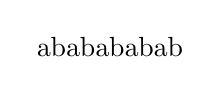
\begin{tikzpicture}
\node[draw=none] at (0,0) {ababababab};
\end{tikzpicture}
\end{center}
}
\only<4>{
Window of size $3$

\vspace{0.3cm}
Words matching \emph{$k$-test vector} $Z = \langle I, F, T, C \rangle$ where::
\begin{itemize}
\item prefixes $I = \{ab\}$
\item suffixes $F = \{ab,ba\}$
\item segments $T = \{aba,abb,bab,bba\}$
\item short strings $C = \{ab\}$
\end{itemize}
\vspace{0.2cm}
\begin{center}
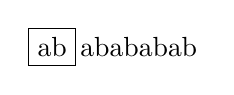
\begin{tikzpicture}
\node[draw] at (0,0) {ab};
\node[draw=none] at (1.1,0) {abababab};
\end{tikzpicture}

\textcolor{green}{ab $\in I$}

\end{center}
}
\only<5>{
Window of size $3$

\vspace{0.3cm}
Words matching \emph{$k$-test vector} $Z = \langle I, F, T, C \rangle$ where::
\begin{itemize}
\item prefixes $I = \{ab\}$
\item suffixes $F = \{ab,ba\}$
\item segments $T = \{aba,abb,bab,bba\}$
\item short strings $C = \{ab\}$
\end{itemize}
\vspace{0.2cm}
\begin{center}
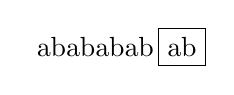
\begin{tikzpicture}
\node[draw=none] at (0,0) {abababab};
\node[draw] at (1.1,0) {ab};
\end{tikzpicture}

\textcolor{green}{ab $\in F$}

\end{center}
}
\only<6>{
Window of size $3$

\vspace{0.3cm}
Words matching \emph{$k$-test vector} $Z = \langle I, F, T, C \rangle$ where::
\begin{itemize}
\item prefixes $I = \{ab\}$
\item suffixes $F = \{ab,ba\}$
\item segments $T = \{aba,abb,bab,bba\}$
\item short strings $C = \{ab\}$
\end{itemize}
\vspace{0.2cm}
\begin{center}
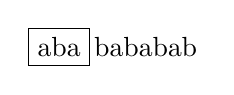
\begin{tikzpicture}
\node[draw] at (0,0) {aba};
\node[draw=none] at (1.1,0) {bababab};
\end{tikzpicture}

\textcolor{green}{aba $\in T$}

\end{center}
}
\only<7>{
Window of size $3$

\vspace{0.3cm}
Words matching \emph{$k$-test vector} $Z = \langle I, F, T, C \rangle$ where::
\begin{itemize}
\item prefixes $I = \{ab\}$
\item suffixes $F = \{ab,ba\}$
\item segments $T = \{aba,abb,bab,bba\}$
\item short strings $C = \{ab\}$
\end{itemize}
\vspace{0.2cm}
\begin{center}
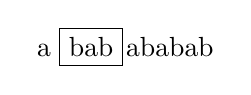
\begin{tikzpicture}
\node[draw=none] at (0,-0.04) {a};
\node[draw] at (0.6,0) {bab};
\node[draw=none] at (1.6,0) {ababab};
\end{tikzpicture}

\textcolor{green}{bab $\in T$}

\end{center}
}
\only<8>{
Window of size $3$

\vspace{0.3cm}
Words matching \emph{$k$-test vector} $Z = \langle I, F, T, C \rangle$ where::
\begin{itemize}
\item prefixes $I = \{ab\}$
\item suffixes $F = \{ab,ba\}$
\item segments $T = \{aba,abb,bab,bba\}$
\item short strings $C = \{ab\}$
\end{itemize}
\vspace{0.2cm}
\begin{center}
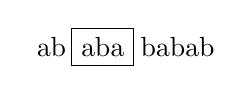
\begin{tikzpicture}
\node[draw=none] at (0,0) {ab};
\node[draw] at (0.65,0) {aba};
\node[draw=none] at (1.6,0) {babab};
\end{tikzpicture}

\textcolor{green}{aba $\in T$}

\end{center}
}
\only<9>{
Window of size $3$

\vspace{0.3cm}
Words matching \emph{$k$-test vector} $Z = \langle I, F, T, C \rangle$ where::
\begin{itemize}
\item prefixes $I = \{ab\}$
\item suffixes $F = \{ab,ba\}$
\item segments $T = \{aba,abb,bab,bba\}$
\item short strings $C = \{ab\}$
\end{itemize}
\vspace{0.2cm}
\begin{center}
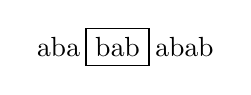
\begin{tikzpicture}
\node[draw=none] at (0,0) {aba};
\node[draw] at (0.75,0) {bab};
\node[draw=none] at (1.6,0) {abab};
\end{tikzpicture}

\textcolor{green}{bab $\in T$}

\end{center}
}
\only<10>{
Window of size $3$

\vspace{0.3cm}
Words matching \emph{$k$-test vector} $Z = \langle I, F, T, C \rangle$ where::
\begin{itemize}
\item prefixes $I = \{ab\}$
\item suffixes $F = \{ab,ba\}$
\item segments $T = \{aba,abb,bab,bba\}$
\item short strings $C = \{ab\}$
\end{itemize}
\vspace{0.2cm}
\begin{center}
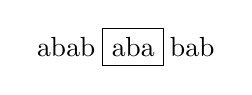
\begin{tikzpicture}
\node[draw=none] at (0,0) {abab};
\node[draw] at (0.85,0) {aba};
\node[draw=none] at (1.6,0) {bab};
\end{tikzpicture}

\textcolor{green}{aba $\in T$}

\end{center}
}
\only<11>{
Window of size $3$

\vspace{0.3cm}
Words matching \emph{$k$-test vector} $Z = \langle I, F, T, C \rangle$ where::
\begin{itemize}
\item prefixes $I = \{ab\}$
\item suffixes $F = \{ab,ba\}$
\item segments $T = \{aba,abb,bab,bba\}$
\item short strings $C = \{ab\}$
\end{itemize}
\vspace{0.2cm}
\begin{center}
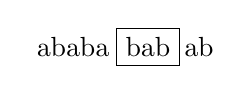
\begin{tikzpicture}
\node[draw=none] at (0,0) {ababa};
\node[draw] at (0.95,0) {bab};
\node[draw=none] at (1.6,0) {ab};
\end{tikzpicture}

\textcolor{green}{bab $\in T$}

\end{center}
}
\only<12>{
Window of size $3$

\vspace{0.3cm}
Words matching \emph{$k$-test vector} $Z = \langle I, F, T, C \rangle$ where::
\begin{itemize}
\item prefixes $I = \{ab\}$
\item suffixes $F = \{ab,ba\}$
\item segments $T = \{aba,abb,bab,bba\}$
\item short strings $C = \{ab\}$
\end{itemize}
\vspace{0.2cm}
\begin{center}
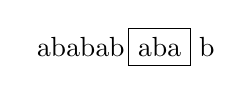
\begin{tikzpicture}
\node[draw=none] at (0,0) {ababab};
\node[draw] at (1.0,0) {aba};
\node[draw=none] at (1.6,0) {b};
\end{tikzpicture}

\textcolor{green}{aba $\in T$}

\end{center}
}
\only<13>{
Window of size $3$

\vspace{0.3cm}
Words matching \emph{$k$-test vector} $Z = \langle I, F, T, C \rangle$ where::
\begin{itemize}
\item prefixes $I = \{ab\}$
\item suffixes $F = \{ab,ba\}$
\item segments $T = \{aba,abb,bab,bba\}$
\item short strings $C = \{ab\}$
\end{itemize}
\vspace{0.2cm}
\begin{center}
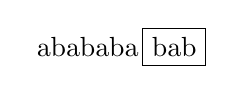
\begin{tikzpicture}
\node[draw=none] at (0,0) {abababa};
\node[draw] at (1.1,0) {bab};
\end{tikzpicture}

\textcolor{green}{bab $\in T$}

\end{center}
}
\only<14>{
Window of size $3$

\vspace{0.3cm}
Words matching \emph{$k$-test vector} $Z = \langle I, F, T, C \rangle$ where::
\begin{itemize}
\item prefixes $I = \{ab\}$
\item suffixes $F = \{ab,ba\}$
\item segments $T = \{aba,abb,bab,bba\}$
\item short strings $C = \{ab\}$
\end{itemize}
\vspace{0.2cm}
\begin{center}
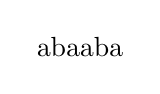
\begin{tikzpicture}
\node[draw=none] at (0,0) {abaaba};
\end{tikzpicture}
\end{center}
}
\only<15>{
Window of size $3$

\vspace{0.3cm}
Words matching \emph{$k$-test vector} $Z = \langle I, F, T, C \rangle$ where::
\begin{itemize}
\item prefixes $I = \{ab\}$
\item suffixes $F = \{ab,ba\}$
\item segments $T = \{aba,abb,bab,bba\}$
\item short strings $C = \{ab\}$
\end{itemize}
\vspace{0.2cm}
\begin{center}
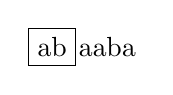
\begin{tikzpicture}
\node[draw] at (0,0) {ab};
\node[draw=none] at (0.7,0) {aaba};
\end{tikzpicture}

\textcolor{green}{ab $\in I$}

\end{center}
}
\only<16>{
Window of size $3$

\vspace{0.3cm}
Words matching \emph{$k$-test vector} $Z = \langle I, F, T, C \rangle$ where::
\begin{itemize}
\item prefixes $I = \{ab\}$
\item suffixes $F = \{ab,ba\}$
\item segments $T = \{aba,abb,bab,bba\}$
\item short strings $C = \{ab\}$
\end{itemize}
\vspace{0.2cm}
\begin{center}
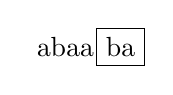
\begin{tikzpicture}
\node[draw=none] at (0,0) {abaa};
\node[draw] at (0.7,0) {ba};
\end{tikzpicture}

\textcolor{green}{ba $\in F$}

\end{center}
}
\only<17>{
Window of size $3$

\vspace{0.3cm}
Words matching \emph{$k$-test vector} $Z = \langle I, F, T, C \rangle$ where::
\begin{itemize}
\item prefixes $I = \{ab\}$
\item suffixes $F = \{ab,ba\}$
\item segments $T = \{aba,abb,bab,bba\}$
\item short strings $C = \{ab\}$
\end{itemize}
\vspace{0.2cm}
\begin{center}
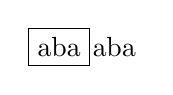
\begin{tikzpicture}
\node[draw] at (0,0) {aba};
\node[draw=none] at (0.7,0) {aba};
\end{tikzpicture}

\textcolor{green}{aba $\in T$}

\end{center}
}
\only<18>{
Window of size $3$

\vspace{0.3cm}
Words matching \emph{$k$-test vector} $Z = \langle I, F, T, C \rangle$ where::
\begin{itemize}
\item prefixes $I = \{ab\}$
\item suffixes $F = \{ab,ba\}$
\item segments $T = \{aba,abb,bab,bba\}$
\item short strings $C = \{ab\}$
\end{itemize}
\vspace{0.2cm}
\begin{center}
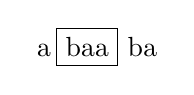
\begin{tikzpicture}
\node[draw=none] at (0,-0.04) {a};
\node[draw] at (0.55,0) {baa};
\node[draw=none] at (1.25,0) {ba};
\end{tikzpicture}

\textcolor{red}{baa $\notin T$}

\end{center}
}
\end{frame}


\begin{frame}{$k$-Testable Languages}

\begin{definition}[from $k$-test vectors to languages]
Let $Z = \langle I, F, T, C \rangle$ be a $k$-test vector, for some $k>0$.
Then
\begin{eqnarray*}
\red{\gamma_k(Z)} & = & C \cup ((I \Sigma^{\ast} \cap \Sigma^{\ast} F) \setminus (\Sigma^{\ast} (\Sigma^k \setminus T)\Sigma^{\ast})).
\end{eqnarray*}
A language $L \subseteq \Sigma^*$ is \red{$k$-testable in the strict sense ($k$-TSS)}\  if there exists a $k$-test vector $Z$ such that $L = \gamma_k (Z)$.
\end{definition}

\only<1>{

Note that $k$-TSS languages are regular.


}\only<2>{
\begin{center}
\scalebox{0.8}{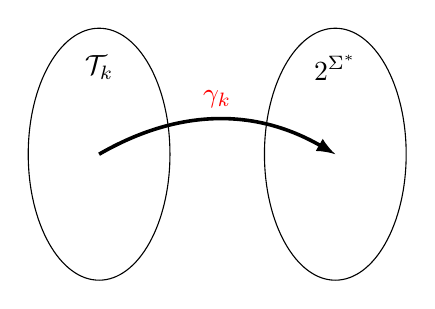
\begin{tikzpicture}
\coordinate (d1) at (0,3.1);
\coordinate (d2) at (3,3.1);
\coordinate (a11) at (0,1.3);
\coordinate (a12) at (0,2);
\coordinate (a21) at (3,1.3);
\coordinate (a22) at (3,2);
\coordinate (gamma) at (1.5,0.6);
\coordinate (alpha) at (1.5,2.7);
%draw (d1) node[] {$({\cal T}_k, \sqsubseteq)$};
%\draw (d2) node[] {$(2^{\Sigma^{\ast}}, \subseteq)$};
\draw (d1) node[] {${\cal T}_k$};
\draw (d2) node[] {$2^{\Sigma^{\ast}}$};
\draw (0,2) ellipse(.9 and 1.6);
\draw (3,2) ellipse(.9 and 1.6);
\draw[>=latex,->,line width=1.3pt] (a12) to[bend left] (a22);
\draw (alpha) node[] {\textcolor{red}{$\gamma_k$}};
\end{tikzpicture}}
\end{center} 
}
\end{frame}












\begin{frame}{$k$-Testable Languages}

\begin{definition}[from Languages to $k$-test vectors]
Let $L \subseteq \Sigma^{\ast}$ be a language and $k > 0$.
Then \red{$\alpha_k (L)$}\  is the $k$-test vector  $\langle I_k(L), F_k(L), T_k(L), C_k(L) \rangle$ where
\begin{itemize}
\item 
$I_k(L) = \{ u \in \Sigma^{k-1} \mid \exists v \in \Sigma^{\ast} : u v \in L \}$,
\item 
$F_k(L) = \{ w \in \Sigma^{k-1} \mid \exists v \in \Sigma^{\ast} : v w \in L \}$,
\item 
$T_k(L) = \{ v \in \Sigma^k \mid \exists u, w \in \Sigma^{\ast} : u v w \in L \}$, and
\item
$C_k(L) = (L \cap \Sigma^{<k-1}) \cup (I_k(L) \cap F_k(L))$.
\end{itemize}
\end{definition}

\pause

\begin{center}
\scalebox{0.7}{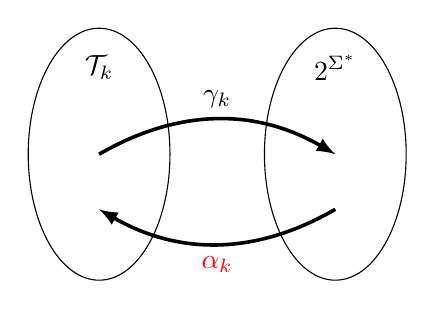
\begin{tikzpicture}
\coordinate (d1) at (0,3.1);
\coordinate (d2) at (3,3.1);
\coordinate (a11) at (0,1.3);
\coordinate (a12) at (0,2);
\coordinate (a21) at (3,1.3);
\coordinate (a22) at (3,2);
\coordinate (gamma) at (1.5,0.6);
\coordinate (alpha) at (1.5,2.7);
%draw (d1) node[] {$({\cal T}_k, \sqsubseteq)$};
%\draw (d2) node[] {$(2^{\Sigma^{\ast}}, \subseteq)$};
\draw (d1) node[] {${\cal T}_k$};
\draw (d2) node[] {$2^{\Sigma^{\ast}}$};
\draw (0,2) ellipse(.9 and 1.6);
\draw (3,2) ellipse(.9 and 1.6);
\draw[>=latex,->,line width=1.3pt] (a12) to[bend left] (a22);
\draw[>=latex,->,line width=1.3pt] (a21) to[bend left] (a11);
\draw (alpha) node[] {$\gamma_k$};
\draw (gamma) node[] {\textcolor{red}{$\alpha_k$}};
\end{tikzpicture}}
\end{center}

\end{frame}






\begin{frame}{$k$-Test Vector Inclusion}

\vspace{0.3cm}

\begin{definition}
Let $k >0$. The relation $\sqsubseteq$ on ${\cal T}_k$ is given by
\begin{eqnarray*}
\langle I, F, T, C \rangle ~\red{\sqsubseteq}~ \langle I', F', T', C' \rangle & \Leftrightarrow & I \subseteq I' \wedge F \subseteq F' \wedge \\
& & ~~~~ T \subseteq T' \wedge C \subseteq C'.
\end{eqnarray*}
\end{definition}

\pause

\begin{center}
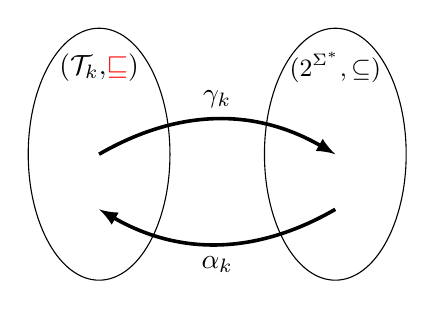
\begin{tikzpicture}
\coordinate (d1) at (0,3.1);
\coordinate (d2) at (3,3.1);
\coordinate (a11) at (0,1.3);
\coordinate (a12) at (0,2);
\coordinate (a21) at (3,1.3);
\coordinate (a22) at (3,2);
\coordinate (gamma) at (1.5,0.6);
\coordinate (alpha) at (1.5,2.7);
%draw (d1) node[] {$({\cal T}_k, \sqsubseteq)$};
%\draw (d2) node[] {$(2^{\Sigma^{\ast}}, \subseteq)$};
\draw (d1) node[] {$({\cal T}_k,$\textcolor{red}{$\sqsubseteq$}$)$};
\draw (d2) node[] {\small{$(2^{\Sigma^{\ast}}, \subseteq)$}};
\draw (0,2) ellipse(.9 and 1.6);
\draw (3,2) ellipse(.9 and 1.6);
\draw[>=latex,->,line width=1.3pt] (a12) to[bend left] (a22);
\draw[>=latex,->,line width=1.3pt] (a21) to[bend left] (a11);
\draw (gamma) node[] {$\alpha_k$};
\draw (alpha) node[] {$\gamma_k$};
\end{tikzpicture}
\end{center}

\end{frame}






\begin{frame}{Order Preservation}


\begin{lemma}
For $k>0$ and for all languages $L, L'$,
\begin{eqnarray*}
L \subseteq L' & \Rightarrow & \alpha_k(L) \sqsubseteq \alpha_k(L').
\end{eqnarray*}
\end{lemma}

\vspace{-0.12cm}

\begin{lemma}
For all $k>0$ and for all $k$-test vectors $Z$ and $Z'$,
\begin{eqnarray*}
Z \sqsubseteq Z' & \Rightarrow & \gamma_k(Z) \subseteq \gamma_k (Z').
\end{eqnarray*}
\end{lemma}

\end{frame}




\begin{frame}{Galois Connection}

\begin{center}
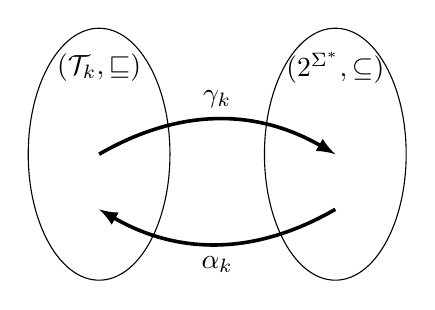
\begin{tikzpicture}
\coordinate (d1) at (0,3.1);
\coordinate (d2) at (3,3.1);
\coordinate (a11) at (0,1.3);
\coordinate (a12) at (0,2);
\coordinate (a21) at (3,1.3);
\coordinate (a22) at (3,2);
\coordinate (gamma) at (1.5,0.6);
\coordinate (alpha) at (1.5,2.7);
%draw (d1) node[] {$({\cal T}_k, \sqsubseteq)$};
%\draw (d2) node[] {$(2^{\Sigma^{\ast}}, \subseteq)$};
\draw (d1) node[] {$({\cal T}_k,\sqsubseteq)$};
\draw (d2) node[] {$(2^{\Sigma^{\ast}},\subseteq)$};
\draw (0,2) ellipse(.9 and 1.6);
\draw (3,2) ellipse(.9 and 1.6);
\draw[>=latex,->,line width=1.3pt] (a12) to[bend left] (a22);
\draw[>=latex,->,line width=1.3pt] (a21) to[bend left] (a11);
\draw (gamma) node[] {$\alpha_k$};
\draw (alpha) node[] {$\gamma_k$};
\end{tikzpicture}
\end{center}

\pause

\vspace{0.3cm}

\begin{theorem}[Galois Connection]
Let $k>0$,  $L \subseteq \Sigma^{\ast}$ a language, and $Z$ a $k$-test vector. Then
\vspace{-0.15cm}
\begin{eqnarray*}
\alpha_k (L) \sqsubseteq Z & \Leftrightarrow & L \subseteq \gamma_k (Z).
\end{eqnarray*}

\end{theorem}

\end{frame}


\frame{
	\frametitle{Galois Connections}
	
	\begin{columns}
		\begin{column}{0.5\textwidth}
			\begin{center}
				\includegraphics[width=0.8\textwidth]{galois_t_shirt}
			\end{center}
		\end{column}
		\begin{column}{0.5\textwidth}
			{\small
				\begin{itemize}
					\item 
					Particular correspondence between two partially ordered sets
					\item
					Many applications in mathematics
					\item
					Adjoint functors in category theory
					\item
					Describe many forms of abstraction in theory of \blue{abstract
						interpretation}\  of programming languages
				\end{itemize}
			}
		\end{column}
	\end{columns}
}

\begin{frame}{Galois Connection}

\begin{corollary}
For all $k>0$, $\gamma_k \circ \alpha_k$ and $\alpha_k \circ \gamma_k$ are monotone and idempotent.
\end{corollary}

Previously established as Theorem 3.2 in \blue{Garcia and Vidal (1990)}\  and as Lemma 3.3 in in \blue{Yokomori and Kobayashi (1998)}.

\end{frame}



\begin{frame}{Galois Connection}

\begin{corollary} 
\label{flationary}
For all $k>0$, $L \subseteq \Sigma^{\ast}$ and $Z \in {\cal T}_k$,
\begin{eqnarray*}
\label{prop1}
\alpha_k \circ \gamma_k (Z) & \sqsubseteq & Z\\
\label{prop2}
L & \subseteq & \gamma_k \circ \alpha_k(L)
\end{eqnarray*}
\end{corollary}

Previously established as Lemma 3.1 in \blue{Garcia and Vidal (1990)}\  and as Lemma 3.1 in \blue{Yokomori and Kobayashi (1998)}.



\end{frame}




\begin{frame}{Galois Connection}


\begin{corollary}
\label{smallestlanguage}
For all $k>0$, $L \subseteq \Sigma^{\ast}$, and $Z \in {\cal T}_k$,
\begin{eqnarray*}
L \subseteq \gamma_k(Z) & \Rightarrow & \gamma_k \circ \alpha_k (L) \subseteq \gamma_k(Z).
\end{eqnarray*}
\end{corollary}

\vspace{0.5cm}

Previously established as Theorem 3.1 in \blue{Garcia and Vidal (1990)}.

\end{frame}







\begin{frame}{Galois Connection}

\begin{corollary}
For all $k>0$ and $Z \in {\cal T}_k$,
$\gamma_k \circ \alpha_k \circ \gamma_k (Z) = \gamma_k(Z)$. Moreover, for any $Z' \in {\cal T}_k$,
\begin{eqnarray*}
\gamma_k(Z) = \gamma_k(Z') & \Rightarrow & \alpha_k \circ \gamma_k (Z) \sqsubseteq Z'.
\end{eqnarray*}
\end{corollary}

\vspace{0.5cm}

Previously established as Lemma 1 in \blue{Yokomori and Kobayashi (1998)}.

\end{frame}










\begin{frame}{Learning $k$-Testable Languages}

\vspace{1.5cm}

\begin{theorem}[Garcia \& Vidal (1990)]
Any $k$-testable language can be identified in the limit from positive examples.
\end{theorem}

\end{frame}


\begin{frame}{Union and Symmetric Difference}

\vspace{0.5cm}

\begin{definition}
The \red{union}\  and \red{symmetric difference}\  of two $k$-test vectors $Z = \langle I, F, T, C\rangle$ and $Z' = \langle I', F', T', C'\rangle$ are given by:
\begin{eqnarray*}
Z \red{\sqcup} Z' & = &  \langle I \cup I', F \cup F', T \cup T', C \cup C' \cup (I \cap F') \cup (I' \cap F) \rangle\\
Z \red{\bigtriangleup} Z' & = &  \langle I \bigtriangleup I', F \bigtriangleup F', T \bigtriangleup T', C \bigtriangleup C' \bigtriangleup (I' \cap F) \bigtriangleup (I \cap F') \rangle
\end{eqnarray*}
\end{definition}

\end{frame}


\begin{frame}{Window Languages Not Closed Under Union}
\vspace{-0.8cm}
\begin{eqnarray*}
Z & = & \langle \{a a\}, \{a a\}, \{a a a\},  \{a a\}\rangle\\
Z' & = & \langle \{b a, b b\}, \{a b, b b \}, \{b a a, b a b, a a a, a a b\}, \{ b b \} \rangle 
\end{eqnarray*}
\vspace{-0.8cm}
\pause
\begin{figure}[h!]
\begin{scriptsize}
\centering     %%% not \center
\captionsetup[subfigure]{position=b}
\subcaptionbox{$\gamma_3(Z)$ and $\gamma_3(Z')$.\label{test:Bild1}}{
\hspace*{1cm}
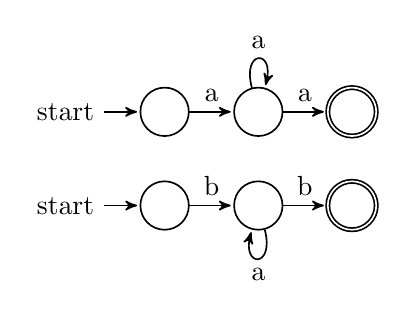
\begin{tikzpicture}[->,shorten >=1pt,auto,node distance=1.7cm,semithick]
\node[initial,state,scale=0.7] (init)                    {};
\node[state,scale=0.7]          (A) [right of=init] {};
\node[state,accepting,scale=0.7]          (AA) [right of=A] {};
\node[initial,state,scale=0.7] (init2)  [below of=init]                  {};
\node[state,scale=0.7]          (B2) [right of=init2] {};
\node[state,accepting,scale=0.7]         (BA2) [right of=B2] {};
\path (init) edge              node {a} (A)
(A)    edge				 node {a} (AA)
(A)   edge [loop above] node {a} (A)
(A)   edge [loop below,draw=none] node {} (A)
(init2) edge [] node {b} (B2)
(B2)    edge	[loop below] node {a} (B2)   
(B2)    edge	[loop above,draw=none] node {}(B2)   
(B2)    edge	[]	node {b} (BA2)
;
\end{tikzpicture}
\hspace*{0.5cm}
}
\subcaptionbox{$\gamma_3(Z) \cup\gamma_3(Z')$.\label{test:Bild2}}{
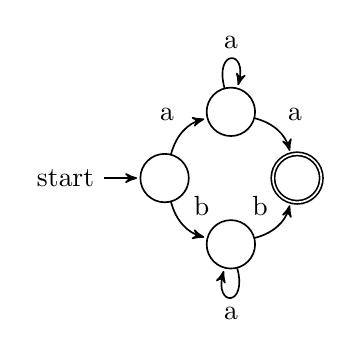
\begin{tikzpicture}[->,shorten >=1pt,auto,node distance=1.7cm,semithick]
\node[initial,state,scale=0.7] (init)                    {};
\node[state,scale=0.7]          			(A) [below right of=init] {};
\node[state,scale=0.7]          (B) [above right of=init] {};
\node[state,accepting,scale=0.7]          (AA) [above right of=A] {};
\path (init) edge  [bend left]            node {a} (B)
(B)    edge	[loop above] node {a} (B)
(B)    edge	[bend left] node {a} (AA)
(init) edge  [bend right]            node {b} (A)
(A) edge  [bend right]            node {b} (AA)
(A) edge  [loop below]            node {a} (A)
;
\end{tikzpicture}
\hspace*{1cm}
}
\end{scriptsize}
\end{figure}
\pause
\begin{center}
$aab \in \gamma_3(Z \sqcup Z')$ but $aab \not\in \gamma_3(Z) \cup \gamma_3(Z')$.
\end{center}

\end{frame}



\begin{frame}{Learning Unions of $k$-Testable Languages}

\vspace{1.5cm}

\begin{theorem}[Identification of unions in the limit]
Any language that is a union of $k$-testable languages can be identified in the limit from positive examples.
\end{theorem}

\end{frame}








\begin{frame}{Distance}

\begin{definition}[Size]
The \red{size}\  of a $k$-test vector $Z = \langle I, F, T, C\rangle$ is defined by:
\begin{eqnarray*}
\red{|Z|} & = |I| + |F| + |T| + |C \cap \Sigma^{<k-1}|.
\end{eqnarray*}
\end{definition}


\begin{definition}[Distance]
We define the \red{distance}\  between a pair of $k$-test vectors as:
\begin{eqnarray*}
\red{d(Z, Z')} & = | Z \bigtriangleup Z' |
\end{eqnarray*}
\end{definition}

\begin{lemma}[Metric]
Distance function  is a metric on the set of $k$-test vectors.
\end{lemma}

\end{frame}



\begin{frame}{Hierarchical Clustering Algorithm}


Given a set $\mathcal{S}$ of words:
\pause
\begin{enumerate}
\item compute $k$-test vectors $s = \{ \alpha_k (\{x\}) \mid x \in \mathcal{S} \}$
\pause
\item compute distance matrix $D$ of  vectors in $s$
\pause
\item until no more merges are possible:
\pause
\begin{enumerate}
\item find closest pair of  vectors $Z$ and $Z'$ s.t. $\gamma_k (Z \sqcup Z') = \gamma_k(Z) \cup \gamma_k(Z')$
\pause
\item replace $Z$ and $Z'$ by  $Z \sqcup Z'$ in $s$
\pause
\item update distance between $Z \sqcup Z'$ and remaining  vectors in $s$
\end{enumerate}

\end{enumerate}

\end{frame}



\begin{frame}{Case Study Oc\'e}
\begin{center}
\tiny
\begin{tabular}{lccr}
\toprule
job & pattern   & 3-test vector & type of job \\ 
\midrule
$\ aaaaa$ 						& \multirow{3}{*}{$a^+$}  	& \multirow{3}{*}{$Z=\langle \{aa\},\{aa\},\{aaa\},\{a,aa\} \rangle$}	& \multirow{3}{*}{homogeneous} \\
\cline{1-1}
\rule{0pt}{2.5ex} $aaaaaaaaaa$ & 						 	&					&				\\
\cline{1-1}
\rule{0pt}{2.5ex} $aaaaa\ldots aaa$ &					&						&			\\
\cline{1-4}
\rule{0pt}{2.5ex} $abababab$	& \multirow{2}{*}{$(ab)^+$} & \multirow{2}{*}{$Z=\langle \{ab\},\{ab\},\{aba,bab\},\{ab\} \rangle$}	& \multirow{4}{*}{heterogeneous} 			\\
\cline{1-1}
\rule{0pt}{2.5ex} $abababababab$	&					& 			&						\\
\cline{1-3}
\rule{0pt}{2.5ex} $abcabcabc$	& \multirow{2}{*}{$(abc)^+$}& 		\multirow{2}{*}{$Z=\langle \{ab\},\{bc\},\{abc,bca,cab\},\{\} \rangle$}						&	\\
\cline{1-1}
\rule{0pt}{2.5ex} $abcabcabcabcabc$ & 					&			&						\\
\cline{1-4}
\rule{0pt}{2.5ex} $abcbcbcbca$ & $a(bc)^+a$ 				& $Z=\langle \{ab\},\{ca\},\{abc,bcb,cbc,cba\},\{\} \rangle$  & booklet \\
\bottomrule
\end{tabular}

\begin{figure}
\vspace{0.3cm}
\includegraphics[width=0.7\linewidth]{2015-03-01-varioprint-i300-2.jpg}
\end{figure}

\end{center}

\end{frame}

\section{Galois Connections for Active Learning}

\frame{
	\frametitle{A Simple Galois Connection for Handling Subalphabets}
	
	\begin{theorem}
		Let, for $i = 1, 2$, $\M_i = \langle I_i, O_i, Q_i, q_i^0, \rightarrow_i \rangle$ be (nondeterministic) Mealy machines with
		$I_1 \supseteq I_2$ and $O_1 = O_2$.
		Then 
		\begin{eqnarray*}
			\M_1 \downarrow I_2 \leq \M_2 & \Leftrightarrow & \M_1 \leq \M_2 \uparrow I_1.
		\end{eqnarray*}
	\end{theorem}
	
	Here $\M_1 \downarrow I_2$ removes all transitions with input label not in $I_2$, and
	$\M_2 \uparrow I_1$ adds transitions to a chaos state for all inputs not in $I_2$.
}


\frame{
	\frametitle{A Galois Connection for Action Refinement}
	Assume we have sets $X$ and $Y$ of \red{abstract}\  inputs and outputs, and sets $I$ and $O$
	of \red{concrete}\  inputs and outputs. An \red{action refinement}\  $\rho$ is a pair of injective functions
	\begin{eqnarray*}
		\rho_i  :  X \rightarrow I^+ &&
		\rho_o  :  Y \rightarrow O^+
	\end{eqnarray*}
	such that $\rho_i(x) \leq \rho_i(x') \Rightarrow x=x'$.
}

\iflong
\frame{
	\frametitle{Respecting an Action Refinement}
	
	%Let $\perp \not\in O$ be a fresh symbol that denotes the undefined output.
	Suppose $\M = \langle I, O, Q, q_0, \rightarrow \rangle$ is a Mealy machine.
	Let $Q_{\rho}\subseteq Q$ be the set of states that can be reached via zero or more $\rho_i$-steps
	from $q_0$.
	So $Q_{\rho}$ is the smallest set satisfying:
	\begin{eqnarray*}
		&& q_0 \in Q_{\rho}\\
		q \in Q_{\rho} \wedge q \stackrel{\rho_i(x)/s}{\Rightarrow} q' & \implies & q'\in Q_{\rho}
	\end{eqnarray*}
	We say that $\M$ \red{respects}\ action refinement $\rho$ if
	\begin{eqnarray*}
		q \in Q_{\rho} \wedge q \stackrel{u/s}{\Rightarrow} q' \wedge u \in {\sf range}(\rho_i) & \implies &  s \in {\sf range}( \rho_o)
	\end{eqnarray*}
}

\frame{
	\frametitle{Abstraction}
	We define the \red{abstraction $\alpha_{\rho}(\M)$}\  to be the Mealy machine
	$\langle X, Y, Q_{\rho}, q_0, \rightarrow_{\rho} \rangle$, where 
	\begin{eqnarray*}
		q \xrightarrow{x/y}_{\rho} q'& \Leftrightarrow & q \stackrel{\rho_i(x)/\rho_o(y)}{\Rightarrow} q'
	\end{eqnarray*}
	Note that $\alpha_{\rho}(\M)$ is input enabled, as required for a Mealy machine: for any $q \in Q_{\rho}$ and $x \in X$, since
	$\M$ is input enabled and by definition of $Q_{\rho}$, there exist a $s\in O^+$ and $q'\in Q_{\rho}$ such that $q \stackrel{\rho_i(x)/s}{\Rightarrow} q'$. Since $\M$ respects $\rho$,
	there exists a $y \in Y$ such that $s = \rho_o(y)$.
}

\frame{
	A Mealy machine $\N= \langle X,Y, Q, q_0, \rightarrow \rangle$ \red{respects}\  action refinement $\rho$ if,
	for every transition $q \xrightarrow{x/y} q'$ of $\N$, $\rho_i(x) = \rho_o(y)$.
}

\frame{
	\frametitle{Concretization}
	We define the \red{concretization $\gamma_{\rho}(\N)$}\  to be the Mealy machine
	$\langle I, O, Q_{\rho}, (q_0, \epsilon, \epsilon), \rightarrow_{\rho} \rangle$ where
	\begin{eqnarray*}
		Q_{\rho} & = & \{ (q, u, s) \in Q \times I^* \times O^* \mid
		\exists x, y : q \xrightarrow{x/y} \wedge \\
		& & ~~~~~~ u < \rho_i(x) \wedge s < \rho_o(y) \wedge |u|=|s| \} \cup \{ \chi \}
	\end{eqnarray*}
	and transition relation $\rightarrow_{\rho}$ comprises the following transitions:
	\begin{eqnarray*}
		(q, u, s) \xrightarrow{i/o} (q, ui, so) &&\\
		(q, u, s) \xrightarrow{i/o} (q', \epsilon, \epsilon) & \mbox{if} & \exists x, y : q \xrightarrow{x/y} q' \wedge \rho_i(x) = ui \wedge \rho_o(y) = s o\\
		(q,u,s) \xrightarrow{i/o} \chi & \mbox{if} &  \neg (\exists x, y : q \xrightarrow{x/y} \wedge ui \leq \rho_i(x))\\
		\chi \xrightarrow{i/o} \chi &&
	\end{eqnarray*}
}
\fi

\frame{
	\frametitle{Galois Connection}
	\iflong
	\begin{lemma}
		$\alpha_{\rho}(\M)$  and $\gamma_{\rho}(\N)$ respect $\rho$.
	\end{lemma}
	
	\begin{lemma}
		$\alpha_{\rho}$ and $\gamma_{\rho}$ are monotone operations.
	\end{lemma}
	\else
	Then we can define monotone abstraction operators $\alpha_{\rho}$ and concretization operators $\gamma_{\rho}$ such that:
	\fi
	
	\begin{theorem}
		Let $\M$ be a Mealy machine over $I$ and $O$, and let $\N$ be a Mealy machine over 
		$X$ and $Y$.
		If $\M$ and $\N$ 
		\iflong
		respect
		\else
		``respect''
		\fi 
		refinement $\rho$ then
		\begin{eqnarray*}
			\alpha_{\rho}(\M) \leq \N & \Leftrightarrow & \M \leq \gamma_{\rho} (\N)
		\end{eqnarray*}
	\end{theorem}
	
}

\frame{
	\frametitle{A Theory of Mappers (AJUV, 2015)}
	
	\begin{center}
		\includegraphics[width=.9\textwidth]{mappers.jpg}
	\end{center}
}

\frame{
	\frametitle{Transducers}
	
	\begin{definition} [Mapper]
		A \red{mapper}\  for a set of inputs $I$ and a set of outputs $O$ is a deterministic Mealy machine
		$\A = \langle I \cup O, X \cup Y,  R, r_0, \delta, \lambda \rangle$, where
		\begin{itemize}
			\item $I$ and $O$ are disjoint sets of \red{concrete input/output symbols},
			\item $X$ and $Y$ are finite sets of \red{abstract input/output symbols}, and
			\item $\lambda : R \times (I \cup O) \rightarrow (X \cup Y)$, the \red{abstraction function},
			respects inputs and outputs, that is, for all $a \in I \cup O$ and $r \in R$, $a \in I \Leftrightarrow \lambda(r,a) \in X$.
		\end{itemize}
	\end{definition}
	
%	We assume that mappers are \red{surjective}: for every state $r$ and every abstract symbol $z$ there is a concrete symbol $a$ with $\lambda(r,a)=z$.
%	(Otherwise we get a useful theory, but no Galois connection.)
}

\iflong
\frame{
	\frametitle{Abstraction}
	
	\begin{definition} [Abstraction]
		Let $\M = \langle I, O, Q, q_0, \rightarrow \rangle$ be a Mealy machine and let
		$\A = \langle I \cup O, X \cup Y, R, r_0, \delta, \lambda \rangle$ be a mapper.
		Then \red{$\alpha_{\A}(\M)$}, the \red{abstraction}\  of $\M$ via $\A$, is the Mealy machine
		$\langle X, Y , Q \times R, (q_0 , r_0), \rightarrow \rangle$, where 
		$\rightarrow$ is given by
		\[
		\frac{q \xrightarrow{i/o} q' ,~ r \xrightarrow{i/x} r' \xrightarrow{o/y} r''}
		{(q, r) \xrightarrow{x/y} (q',r'')}
		\]
	\end{definition}
}

\frame{
	\frametitle{Concretization}
	
	\begin{definition} [Concretization]
		
		Let ${\cal H} = \langle X, Y \cup \{ \perp \}, H, h_0, \rightarrow \rangle$ be a Mealy machine and let
		$\A = \langle I \cup O, X \cup Y, R, r_0, \delta, \lambda \rangle$ be a mapper for $I$ and $O$.
		Then \red{$\gamma_{\A}({\cal H})$}, the \red{concretization}\  of ${\cal H}$ via $\A$, is the Mealy machine
		$\langle I, O, R \times H, (r_0, h_0), \rightarrow \rangle$, where $\rightarrow$ is given by 
		\[
		\frac
		{r \xrightarrow{i/x} r' \xrightarrow{o/y} r'' ,~ h \xrightarrow{x/y} h'}
		{(r, h) \xrightarrow{i/o} (r'', h')}
		\]
	\end{definition}
}
\fi

\frame{
	\frametitle{A Galois Connection that is Quite Useful}
	To every mapper ${\cal A}$ we may associate an abstraction operator $\alpha_{\cal A}$ and a concretization operator $\gamma_{\cal A}$. Then
	\begin{theorem}
		For a ``surjective'' mapper ${\cal A}$ and (nondeterministic) Mealy machines ${\cal M}$ and ${\cal H}$,
		\begin{eqnarray*}
			\alpha_{\cal A}({\cal M}) \leq {\cal H} & \Leftrightarrow & 
			{\cal M} \leq \gamma_{\cal A}({\cal H})  
		\end{eqnarray*}
	\end{theorem}
}











\section{Conclusions and Future Work}
\frame{
	\frametitle{Conclusions}
	Automata learning is emerging as a highly effective bug-finding technique,
	and  slowly becoming a standard tool in the toolbox of the software engineer.
	
%	\vspace{1 em}
%	Galois connections provide useful abstractions.
%	
%	\vspace{1 em}
%	Further research needed!
}

\frame{
	\frametitle{Future Work}
	\begin{enumerate}
		\item
		Improved algorithms for black-box learning/testing FSMs	
		\item
		Better understanding of role Galois connections in learning;
		algorithms for finding Galois connections automatically
		\item
		From Mealy machines to I/O automata
		\item
		Learning EFSMs
		\item
		Combinations of black-box and white-box learning
		\item
		Algorithms for models with time and probabilities
		\item
		Refactoring of legacy software excellent application domain
	\end{enumerate}
}







\end{document}
